% svn info. These are modified by svn at checkout time.
% The last version of these macros found before the maketitle will be the one on the front page,
% so only the main file is tracked.
% Do not edit by hand!
\RCS$Revision: 61320 $
\RCS$HeadURL: svn+ssh://svn.cern.ch/reps/tdr2/notes/AN-10-108/trunk/AN-10-108.tex $
\RCS$Id: AN-10-108.tex 61320 2011-06-15 15:39:59Z rharris $
%%%%%%%%%%%%% ptdr definitions %%%%%%%%%%%%%%%%%%%%%
\def\Fileversion$#1: #2 ${\gdef\fileversion{#2}}
\def\Filedate$#1: #2-#3-#4 #5 ${\gdef\filedate{#2/#3/#4}}
\Fileversion$Revision: 227897 $
\Filedate$Date: 2014-02-16 08:24:34 -0600 (Sun, 16 Feb 2014) $
%%%%%%%%%%%%%%%%%%%%%%%%%%%%%%%%%%%%%%%%%%%%%%%%%%%%%%%%%%%%%%%%%%%%
%
%  CMS Common definitions style file
%
%  N.B. use of \newcommand rather than \newcommand means
%       that a definition is ignored if already specified
%
%                                              L. Taylor 18 Feb 2005
%%%%%%%%%%%%%%%%%%%%%%%%%%%%%%%%%%%%%%%%%%%%%%%%%%%%%%%%%%%%%%%%%%%%
\NeedsTeXFormat{LaTeX2e}
\ProvidesPackage{ptdr-definitions}[\filedate\space CMS Additional Macro Definitions (\fileversion)]
\RequirePackage{xspace}
\RequirePackage{amsmath}

% Some shorthand
% turn off italics
\newcommand {\etal}{\mbox{et al.}\xspace} %et al. - no preceding comma
\newcommand {\ie}{\mbox{i.e.}\xspace}     %i.e.
\newcommand {\eg}{\mbox{e.g.}\xspace}     %e.g.
\newcommand {\etc}{\mbox{etc.}\xspace}     %etc.
\newcommand {\vs}{\mbox{\sl vs.}\xspace}      %vs.
\newcommand {\mdash}{\ensuremath{\mathrm{-}}} % for use within formulas

% some terms whose definition we may change
\newcommand {\Lone}{Level-1\xspace} % Level-1 or L1 ?
\newcommand {\Ltwo}{Level-2\xspace}
\newcommand {\Lthree}{Level-3\xspace}

% Some software programs (alphabetized)
\newcommand{\ACERMC} {\textsc{AcerMC}\xspace}
\newcommand{\ALPGEN} {{\textsc{alpgen}}\xspace}
\newcommand{\CALCHEP} {{\textsc{CalcHEP}}\xspace}
\newcommand{\CHARYBDIS} {{\textsc{charybdis}}\xspace}
\newcommand{\CMKIN} {\textsc{cmkin}\xspace}
\newcommand{\CMSIM} {{\textsc{cmsim}}\xspace}
\newcommand{\CMSSW} {{\textsc{cmssw}}\xspace}
\newcommand{\COBRA} {{\textsc{cobra}}\xspace}
\newcommand{\COCOA} {{\textsc{cocoa}}\xspace}
\newcommand{\COMPHEP} {\textsc{CompHEP}\xspace}
\newcommand{\EVTGEN} {{\textsc{evtgen}}\xspace}
\newcommand{\FAMOS} {{\textsc{famos}}\xspace}
\newcommand{\GARCON} {\textsc{garcon}\xspace}
\newcommand{\GARFIELD} {{\textsc{garfield}}\xspace}
\newcommand{\GEANE} {{\textsc{geane}}\xspace}
\newcommand{\GEANTfour} {{\textsc{Geant4}}\xspace}
\newcommand{\GEANTthree} {{\textsc{geant3}}\xspace}
\newcommand{\GEANT} {{\textsc{geant}}\xspace}
\newcommand{\HDECAY} {\textsc{hdecay}\xspace}
\newcommand{\HERWIG} {{\textsc{herwig}}\xspace}
\newcommand{\HERWIGpp} {{\textsc{herwig++}}\xspace}
\newcommand{\POWHEG} {{\textsc{powheg}}\xspace}
\newcommand{\HIGLU} {{\textsc{higlu}}\xspace}
\newcommand{\HIJING} {{\textsc{hijing}}\xspace}
\newcommand{\IGUANA} {\textsc{iguana}\xspace}
\newcommand{\ISAJET} {{\textsc{isajet}}\xspace}
\newcommand{\ISAPYTHIA} {{\textsc{isapythia}}\xspace}
\newcommand{\ISASUGRA} {{\textsc{isasugra}}\xspace}
\newcommand{\ISASUSY} {{\textsc{isasusy}}\xspace}
\newcommand{\ISAWIG} {{\textsc{isawig}}\xspace}
\newcommand{\MADGRAPH} {\textsc{MadGraph}\xspace}
\newcommand{\MCATNLO} {\textsc{mc@nlo}\xspace}
\newcommand{\MCFM} {\textsc{mcfm}\xspace}
\newcommand{\MILLEPEDE} {{\textsc{millepede}}\xspace}
\newcommand{\ORCA} {{\textsc{orca}}\xspace}
\newcommand{\OSCAR} {{\textsc{oscar}}\xspace}
\newcommand{\PHOTOS} {\textsc{photos}\xspace}
\newcommand{\PROSPINO} {\textsc{prospino}\xspace}
\newcommand{\PYTHIA} {{\textsc{pythia}}\xspace}
\newcommand{\SHERPA} {{\textsc{sherpa}}\xspace}
\newcommand{\TAUOLA} {\textsc{tauola}\xspace}
\newcommand{\TOPREX} {\textsc{TopReX}\xspace}
\newcommand{\XDAQ} {{\textsc{xdaq}}\xspace}


%  Experiments
\newcommand {\DZERO}{D0\xspace}     %etc.


% Measurements and units...

\newcommand{\de}{\ensuremath{^\circ}}
\newcommand{\ten}[1]{\ensuremath{\times \text{10}^\text{#1}}}
\newcommand{\unit}[1]{\ensuremath{\text{\,#1}}\xspace}
\newcommand{\mum}{\ensuremath{\,\mu\text{m}}\xspace}
\newcommand{\micron}{\ensuremath{\,\mu\text{m}}\xspace}
\newcommand{\cm}{\ensuremath{\,\text{cm}}\xspace}
\newcommand{\mm}{\ensuremath{\,\text{mm}}\xspace}
\newcommand{\mus}{\ensuremath{\,\mu\text{s}}\xspace}
\newcommand{\keV}{\ensuremath{\,\text{ke\hspace{-.08em}V}}\xspace}
\newcommand{\MeV}{\ensuremath{\,\text{Me\hspace{-.08em}V}}\xspace}
\newcommand{\MeVns}{\ensuremath{\text{Me\hspace{-.08em}V}}\xspace} % no leading thinspace
\newcommand{\GeV}{\ensuremath{\,\text{Ge\hspace{-.08em}V}}\xspace}
\newcommand{\GeVns}{\ensuremath{\text{Ge\hspace{-.08em}V}}\xspace} % no leading thinspace
\newcommand{\gev}{\GeV}
\newcommand{\TeV}{\ensuremath{\,\text{Te\hspace{-.08em}V}}\xspace}
\newcommand{\TeVns}{\ensuremath{\text{Te\hspace{-.08em}V}}\xspace} % no leading thinspace
\newcommand{\PeV}{\ensuremath{\,\text{Pe\hspace{-.08em}V}}\xspace}
\newcommand{\keVc}{\ensuremath{{\,\text{ke\hspace{-.08em}V\hspace{-0.16em}/\hspace{-0.08em}}c}}\xspace}
\newcommand{\MeVc}{\ensuremath{{\,\text{Me\hspace{-.08em}V\hspace{-0.16em}/\hspace{-0.08em}}c}}\xspace}
\newcommand{\GeVc}{\ensuremath{{\,\text{Ge\hspace{-.08em}V\hspace{-0.16em}/\hspace{-0.08em}}c}}\xspace}
\newcommand{\GeVcns}{\ensuremath{{\text{Ge\hspace{-.08em}V\hspace{-0.16em}/\hspace{-0.08em}}c}}\xspace} % no leading thinspace
\newcommand{\TeVc}{\ensuremath{{\,\text{Te\hspace{-.08em}V\hspace{-0.16em}/\hspace{-0.08em}}c}}\xspace}
\newcommand{\keVcc}{\ensuremath{{\,\text{ke\hspace{-.08em}V\hspace{-0.16em}/\hspace{-0.08em}}c^\text{2}}}\xspace}
\newcommand{\MeVcc}{\ensuremath{{\,\text{Me\hspace{-.08em}V\hspace{-0.16em}/\hspace{-0.08em}}c^\text{2}}}\xspace}
\newcommand{\GeVcc}{\ensuremath{{\,\text{Ge\hspace{-.08em}V\hspace{-0.16em}/\hspace{-0.08em}}c^\text{2}}}\xspace}
\newcommand{\GeVccns}{\ensuremath{{\text{Ge\hspace{-.08em}V\hspace{-0.16em}/\hspace{-0.08em}}c^\text{2}}}\xspace} % no leading thinspace
\newcommand{\TeVcc}{\ensuremath{{\,\text{Te\hspace{-.08em}V\hspace{-0.16em}/\hspace{-0.08em}}c^\text{2}}}\xspace}

\newcommand{\pbinv} {\mbox{\ensuremath{\,\text{pb}^\text{$-$1}}}\xspace}
\newcommand{\fbinv} {\mbox{\ensuremath{\,\text{fb}^\text{$-$1}}}\xspace}
\newcommand{\nbinv} {\mbox{\ensuremath{\,\text{nb}^\text{$-$1}}}\xspace}
\newcommand{\mubinv} {\ensuremath{\,\mu\mathrm{b}^{-1}}\xspace}
\newcommand{\percms}{\ensuremath{\,\text{cm}^\text{$-$2}\,\text{s}^\text{$-$1}}\xspace}
\newcommand{\lumi}{\ensuremath{\mathcal{L}}\xspace}
\newcommand{\Lumi}{\ensuremath{\mathcal{L}}\xspace}%both upper and lower
%
% Need a convention here:
\newcommand{\LvLow}  {\ensuremath{\mathcal{L}=\text{10}^\text{32}\,\text{cm}^\text{$-$2}\,\text{s}^\text{$-$1}}\xspace}
\newcommand{\LLow}   {\ensuremath{\mathcal{L}=\text{10}^\text{33}\,\text{cm}^\text{$-$2}\,\text{s}^\text{$-$1}}\xspace}
\newcommand{\lowlumi}{\ensuremath{\mathcal{L}=\text{2}\times \text{10}^\text{33}\,\text{cm}^\text{$-$2}\,\text{s}^\text{$-$1}}\xspace}
\newcommand{\LMed}   {\ensuremath{\mathcal{L}=\text{2}\times \text{10}^\text{33}\,\text{cm}^\text{$-$2}\,\text{s}^\text{$-$1}}\xspace}
\newcommand{\LHigh}  {\ensuremath{\mathcal{L}=\text{10}^\text{34}\,\text{cm}^\text{$-$2}\,\text{s}^\text{$-$1}}\xspace}
\newcommand{\hilumi} {\ensuremath{\mathcal{L}=\text{10}^\text{34}\,\text{cm}^\text{$-$2}\,\text{s}^\text{$-$1}}\xspace}

% Physics symbols ...

\newcommand{\PT}{\ensuremath{p_{\mathrm{T}}}\xspace}
\newcommand{\pt}{\ensuremath{p_{\mathrm{T}}}\xspace}
\newcommand{\ET}{\ensuremath{E_{\mathrm{T}}}\xspace}
\newcommand{\HT}{\ensuremath{H_{\mathrm{T}}}\xspace}
\newcommand{\et}{\ensuremath{E_{\mathrm{T}}}\xspace}
\newcommand{\Em}{\ensuremath{E\hspace{-0.6em}/}\xspace}
\newcommand{\Pm}{\ensuremath{p\hspace{-0.5em}/}\xspace}
\newcommand{\PTm}{\ensuremath{{p}_\mathrm{T}\hspace{-1.02em}/\kern 0.5em}\xspace}
\newcommand{\PTslash}{\PTm}
\newcommand{\ETm}{\ensuremath{E_{\mathrm{T}}^{\text{miss}}}\xspace}
\newcommand{\MET}{\ETm}
\newcommand{\ETmiss}{\ETm}
\newcommand{\ETslash}{\ensuremath{E_{\mathrm{T}}\hspace{-1.1em}/\kern0.45em}\xspace}
\newcommand{\VEtmiss}{\ensuremath{{\vec E}_{\mathrm{T}}^{\text{miss}}}\xspace}
\newcommand{\ptvec}{\ensuremath{{\vec p}_{\mathrm{T}}}\xspace}

% roman face derivative
\newcommand{\dd}[2]{\ensuremath{\frac{\cmsSymbolFace{d} #1}{\cmsSymbolFace{d} #2}}}
\newcommand{\ddinline}[2]{\ensuremath{\cmsSymbolFace{d} #1/\cmsSymbolFace{d} #2}}
\newcommand{\rd}{\ensuremath{\cmsSymbolFace{d}}}
\newcommand{\re}{\ensuremath{\cmsSymbolFace{e}}}
% absolute value
\newcommand{\abs}[1]{\ensuremath{\lvert #1 \rvert}}



\ifthenelse{\boolean{cms@italic}}{\newcommand{\cmsSymbolFace}{\relax}}{\newcommand{\cmsSymbolFace}{\mathrm}}

% Particle names which track the italic/non-italic face convention
\newcommand{\zp}{\ensuremath{\cmsSymbolFace{Z}^\prime}\xspace} % plain Z'
\newcommand{\JPsi}{\ensuremath{\cmsSymbolFace{J}\hspace{-.08em}/\hspace{-.14em}\psi}\xspace} % J/Psi (no mass)
\newcommand{\Z}{\ensuremath{\cmsSymbolFace{Z}}\xspace} % plain Z (no superscript 0)
\newcommand{\ttbar}{\ensuremath{\cmsSymbolFace{t}\overline{\cmsSymbolFace{t}}}\xspace} % t-tbar

% Extensions for missing names in PENNAMES % note no xspace, to match syntax in PENNAMES
\newcommand{\cPgn}{\ensuremath{\nu}} % generic neutrino
\providecommand{\Pgn}{\ensuremath{\nu}} % generic neutrino
\newcommand{\cPagn}{\ensuremath{\overline{\nu}}} % generic neutrino
\providecommand{\Pagn}{\ensuremath{\overline{\nu}}} % generic neutrino
\newcommand{\cPgg}{\ensuremath{\gamma}} % gamma
\newcommand{\cPJgy}{\ensuremath{\cmsSymbolFace{J}\hspace{-.08em}/\hspace{-.14em}\psi}} % J/Psi (no mass)
\newcommand{\cPZ}{\ensuremath{\cmsSymbolFace{Z}}} % plain Z (no superscript 0)
\newcommand{\cPZpr}{\ensuremath{\cmsSymbolFace{Z}^\prime}} % plain Z'
\newcommand{\cPqt}{\ensuremath{\cmsSymbolFace{t}}} % t for t quark
\newcommand{\cPqb}{\ensuremath{\cmsSymbolFace{b}}} % b for b quark
\newcommand{\cPqc}{\ensuremath{\cmsSymbolFace{c}}} % c for c quark
\newcommand{\cPqs}{\ensuremath{\cmsSymbolFace{s}}} % s for s quark
\newcommand{\cPqu}{\ensuremath{\cmsSymbolFace{u}}} % u for u quark
\newcommand{\cPqd}{\ensuremath{\cmsSymbolFace{d}}} % d for d quark
\newcommand{\cPq}{\ensuremath{\cmsSymbolFace{q}}} % generic quark
\newcommand{\cPg}{\ensuremath{\cmsSymbolFace{g}}} % generic gluon
\newcommand{\cPG}{\ensuremath{\cmsSymbolFace{G}}} % Graviton
\newcommand{\cPaqt}{\ensuremath{\overline{\cmsSymbolFace{t}}}} % t for t anti-quark
\newcommand{\cPaqb}{\ensuremath{\overline{\cmsSymbolFace{b}}}} % b for b anti-quark
\newcommand{\cPaqc}{\ensuremath{\overline{\cmsSymbolFace{c}}}} % c for c anti-quark
\newcommand{\cPaqs}{\ensuremath{\overline{\cmsSymbolFace{s}}}} % s for s anti-quark
\newcommand{\cPaqu}{\ensuremath{\overline{\cmsSymbolFace{u}}}} % u for u anti-quark
\newcommand{\cPaqd}{\ensuremath{\overline{\cmsSymbolFace{d}}}} % d for d anti-quark
\newcommand{\cPaq}{\ensuremath{\overline{\cmsSymbolFace{q}}}} % generic anti-quark
\newcommand{\cPKstz}{\ensuremath{\cmsSymbolFace{K}^{\ast0}}\xspace} %note has xspace
% future symbols from heppennames2
\providecommand{\PH}{\ensuremath{\cmsSymbolFace{H}}\xspace} % plain Higgs
\providecommand{\PJGy}{\ensuremath{\cmsSymbolFace{J}\hspace{-.08em}/\hspace{-.14em}\psi}\xspace} % J/Psi (no mass)
\providecommand{\PBzs}{\ensuremath{\cmsSymbolFace{B}^0_\cmsSymbolFace{s}}\xspace} % B^0_s
\providecommand{\Pg}{\ensuremath{\cmsSymbolFace{g}}\xspace} % generic gluon
\providecommand{\PSg}{\ensuremath{\widetilde{\cmsSymbolFace{g}}}\xspace} % gluino
\providecommand{\PSQ}{\ensuremath{\widetilde{\cmsSymbolFace{q}}}\xspace} % squark
\providecommand{\PXXG}{\ensuremath{\cmsSymbolFace{G}}\xspace} % graviton
\providecommand{\PXXSG}{\ensuremath{\widetilde{\PXXG}}\xspace} % gravitino
\providecommand{\PSGcp}{\ensuremath{\widetilde{\chi}^+}\xspace}
\providecommand{\PSGc}{\ensuremath{\widetilde{\chi}}\xspace} % neutralino
\providecommand{\PSGcz}{\ensuremath{\widetilde{\chi}^0}\xspace} % neutralino with superscript 0
\providecommand{\PSGczDo}{\ensuremath{\widetilde{\chi}^{0}_{1}}\xspace} % neutralino
\providecommand{\PSGczDt}{\ensuremath{\widetilde{\chi}^{0}_{2}}\xspace} % neutralino
\providecommand{\PSGcpm}{\ensuremath{\widetilde{\chi}^\pm}\xspace} % neutralino
\providecommand{\Pl}{\ensuremath{\cmsSymbolFace{l}}\xspace} % non-ell lepton
\providecommand{\PAl}{\ensuremath{\overline{\cmsSymbolFace{l}}}\xspace} % non-ell anti-lepton
\providecommand{\PGnl}{\ensuremath{\nu_\cmsSymbolFace{l}}\xspace} % lepton neutrino
\providecommand{\PAGnl}{\ensuremath{\overline{\nu}_\cmsSymbolFace{l}}\xspace} % anti-lepton neutrino
\providecommand{\PQtpr}{\ensuremath{\cmsSymbolFace{t}^{\prime}}\xspace} % t'
\providecommand{\PAQtpr}{\ensuremath{\bar{\cmsSymbolFace{t}}^\prime}\xspace} % t'-bar; needs to be converted to overline-requires rework a la heppennames
\providecommand{\PQbpr}{\ensuremath{\cmsSymbolFace{b}^{\prime}}\xspace} % b'
\providecommand{\PAQbpr}{\ensuremath{\bar{\cmsSymbolFace{b}}^\prime}\xspace} % b'-bar; needs same as anti-t'
\providecommand{\PGg}{\ensuremath{\gamma}\xspace} % gamma
\providecommand{\PKzS}{\ensuremath{\cmsSymbolFace{K}^0_\cmsSymbolFace{S}}\xspace} % K short
\providecommand{\PBs}{\ensuremath{\cmsSymbolFace{B}_\cmsSymbolFace{s}}\xspace} % B sub s
\providecommand{\PSQt}{\ensuremath{\widetilde{\cmsSymbolFace{t}}}\xspace} % stop
\providecommand{\PZpr}{\ensuremath{\cmsSymbolFace{Z}^\prime}\xspace} % plain Z'
\providecommand{\PWpr}{\ensuremath{\cmsSymbolFace{W}^\prime}\xspace} % plain W'
\providecommand{\PGn}{\ensuremath{\nu}\xspace} % generic neutrino
\providecommand{\PAGn}{\ensuremath{\overline{\nu}}\xspace} % generic neutrino


% for APS style tables
\ifthenelse{\boolean{cms@external}}{%
\newenvironment{scotch}[1]{\protect\centering\ruledtabular\tabular{#1}}{\endtabular\endruledtabular}
}{
\newenvironment{scotch}[1]{\protect\centering\tabular{#1}\hline\hline}{\hline\endtabular}
}

% SM (still to be classified)

\newcommand{\AFB}{\ensuremath{A_\text{FB}}\xspace}
\newcommand{\wangle}{\ensuremath{\sin^{2}\theta_{\text{eff}}^\text{lept}(M^2_{\Z})}\xspace}
\newcommand{\stat}{\ensuremath{\,\text{(stat.)}}\xspace}
\newcommand{\syst}{\ensuremath{\,\text{(syst.)}}\xspace}
\newcommand{\lum}{\ensuremath{\,\text{(lum.)}}\xspace}
\newcommand{\kt}{\ensuremath{k_{\mathrm{T}}}\xspace}

\newcommand{\BC}{\ensuremath{\cmsSymbolFace{B_{c}}}\xspace}
\newcommand{\bbarc}{\ensuremath{\cPqb\cPaqc}\xspace}
\newcommand{\bbbar}{\ensuremath{\cPqb\cPaqb}\xspace}
\newcommand{\ccbar}{\ensuremath{\cPqc\cPaqc}\xspace}
\newcommand{\bspsiphi}{\ensuremath{\cmsSymbolFace{B_s} \to \JPsi\, \phi}\xspace}
\newcommand{\EE}{\ensuremath{\Pep\Pem}\xspace}
\newcommand{\MM}{\ensuremath{\Pgmp\Pgmm}\xspace}
\newcommand{\TT}{\ensuremath{\Pgt^{+}\Pgt^{-}}\xspace}

%%%  E-gamma definitions
\newcommand{\HGG}{\ensuremath{\cmsSymbolFace{H}\to\gamma\gamma}}
\newcommand{\GAMJET}{\ensuremath{\gamma + \text{jet}}}
\newcommand{\PPTOJETS}{\ensuremath{\Pp\Pp\to\text{jets}}}
\newcommand{\PPTOGG}{\ensuremath{\Pp\Pp\to\gamma\gamma}}
\newcommand{\PPTOGAMJET}{\ensuremath{\Pp\Pp\to\gamma + \mathrm{jet}}}
\newcommand{\MH}{\ensuremath{M_{\PH}}}
\newcommand{\RNINE}{\ensuremath{R_\mathrm{9}}}
\newcommand{\DR}{\ensuremath{\Delta R}}





%%%%%%
% From Albert
%

\newcommand{\ga}{\ensuremath{\gtrsim}}
\newcommand{\la}{\ensuremath{\lesssim}}
%
\newcommand{\swsq}{\ensuremath{\sin^2\theta_\cmsSymbolFace{W}}\xspace}
\newcommand{\cwsq}{\ensuremath{\cos^2\theta_\cmsSymbolFace{W}}\xspace}
\newcommand{\tanb}{\ensuremath{\tan\beta}\xspace}
\newcommand{\tanbsq}{\ensuremath{\tan^{2}\beta}\xspace}
\newcommand{\sidb}{\ensuremath{\sin 2\beta}\xspace}
\newcommand{\alpS}{\ensuremath{\alpha_S}\xspace}
\newcommand{\alpt}{\ensuremath{\tilde{\alpha}}\xspace}

\newcommand{\QL}{\ensuremath{\cmsSymbolFace{Q}_\cmsSymbolFace{L}}\xspace}
\newcommand{\sQ}{\ensuremath{\widetilde{\cmsSymbolFace{Q}}}\xspace}
\newcommand{\sQL}{\ensuremath{\widetilde{\cmsSymbolFace{Q}}_\cmsSymbolFace{L}}\xspace}
\newcommand{\ULC}{\ensuremath{\cmsSymbolFace{U}_\cmsSymbolFace{L}^\cmsSymbolFace{C}}\xspace}
\newcommand{\sUC}{\ensuremath{\widetilde{\cmsSymbolFace{U}}^\cmsSymbolFace{C}}\xspace}
\newcommand{\sULC}{\ensuremath{\widetilde{\cmsSymbolFace{U}}_\cmsSymbolFace{L}^\cmsSymbolFace{C}}\xspace}
\newcommand{\DLC}{\ensuremath{\cmsSymbolFace{D}_\cmsSymbolFace{L}^\cmsSymbolFace{C}}\xspace}
\newcommand{\sDC}{\ensuremath{\widetilde{\cmsSymbolFace{D}}^\cmsSymbolFace{C}}\xspace}
\newcommand{\sDLC}{\ensuremath{\widetilde{\cmsSymbolFace{D}}_\cmsSymbolFace{L}^\cmsSymbolFace{C}}\xspace}
\newcommand{\LL}{\ensuremath{\cmsSymbolFace{L}_\cmsSymbolFace{L}}\xspace}
\newcommand{\sL}{\ensuremath{\widetilde{\cmsSymbolFace{L}}}\xspace}
\newcommand{\sLL}{\ensuremath{\widetilde{\cmsSymbolFace{L}}_\cmsSymbolFace{L}}\xspace}
\newcommand{\ELC}{\ensuremath{\cmsSymbolFace{E}_\cmsSymbolFace{L}^\cmsSymbolFace{C}}\xspace}
\newcommand{\sEC}{\ensuremath{\widetilde{\cmsSymbolFace{E}}^\cmsSymbolFace{C}}\xspace}
\newcommand{\sELC}{\ensuremath{\widetilde{\cmsSymbolFace{E}}_\cmsSymbolFace{L}^\cmsSymbolFace{C}}\xspace}
\newcommand{\sEL}{\ensuremath{\widetilde{\cmsSymbolFace{E}}_\cmsSymbolFace{L}}\xspace}
\newcommand{\sER}{\ensuremath{\widetilde{\cmsSymbolFace{E}}_\cmsSymbolFace{R}}\xspace}
\newcommand{\sFer}{\ensuremath{\widetilde{\cmsSymbolFace{f}}}\xspace}
\newcommand{\sQua}{\ensuremath{\widetilde{\cmsSymbolFace{q}}}\xspace}
\newcommand{\sUp}{\ensuremath{\widetilde{\cmsSymbolFace{u}}}\xspace}
\newcommand{\suL}{\ensuremath{\widetilde{\cmsSymbolFace{u}}_\cmsSymbolFace{L}}\xspace}
\newcommand{\suR}{\ensuremath{\widetilde{\cmsSymbolFace{u}}_\cmsSymbolFace{R}}\xspace}
\newcommand{\sDw}{\ensuremath{\widetilde{\cmsSymbolFace{d}}}\xspace}
\newcommand{\sdL}{\ensuremath{\widetilde{\cmsSymbolFace{d}}_\cmsSymbolFace{L}}\xspace}
\newcommand{\sdR}{\ensuremath{\widetilde{\cmsSymbolFace{d}}_\cmsSymbolFace{R}}\xspace}
\newcommand{\sTop}{\ensuremath{\widetilde{\cmsSymbolFace{t}}}\xspace}
\newcommand{\stL}{\ensuremath{\widetilde{\cmsSymbolFace{t}}_\cmsSymbolFace{L}}\xspace}
\newcommand{\stR}{\ensuremath{\widetilde{\cmsSymbolFace{t}}_\cmsSymbolFace{R}}\xspace}
\newcommand{\stone}{\ensuremath{\widetilde{\cmsSymbolFace{t}}_1}\xspace}
\newcommand{\sttwo}{\ensuremath{\widetilde{\cmsSymbolFace{t}}_2}\xspace}
\newcommand{\sBot}{\ensuremath{\widetilde{\cmsSymbolFace{b}}}\xspace}
\newcommand{\sbL}{\ensuremath{\widetilde{\cmsSymbolFace{b}}_\cmsSymbolFace{L}}\xspace}
\newcommand{\sbR}{\ensuremath{\widetilde{\cmsSymbolFace{b}}_\cmsSymbolFace{R}}\xspace}
\newcommand{\sbone}{\ensuremath{\widetilde{\cmsSymbolFace{b}}_1}\xspace}
\newcommand{\sbtwo}{\ensuremath{\widetilde{\cmsSymbolFace{b}}_2}\xspace}
\newcommand{\sLep}{\ensuremath{\widetilde{\cmsSymbolFace{l}}}\xspace}
\newcommand{\sLepC}{\ensuremath{\widetilde{\cmsSymbolFace{l}}^\cmsSymbolFace{C}}\xspace}
\newcommand{\sEl}{\ensuremath{\widetilde{\cmsSymbolFace{e}}}\xspace}
\newcommand{\sElC}{\ensuremath{\widetilde{\cmsSymbolFace{e}}^\cmsSymbolFace{C}}\xspace}
\newcommand{\seL}{\ensuremath{\widetilde{\cmsSymbolFace{e}}_\cmsSymbolFace{L}}\xspace}
\newcommand{\seR}{\ensuremath{\widetilde{\cmsSymbolFace{e}}_\cmsSymbolFace{R}}\xspace}
\newcommand{\snL}{\ensuremath{\widetilde{\nu}_L}\xspace}
\newcommand{\sMu}{\ensuremath{\widetilde{\mu}}\xspace}
\newcommand{\sNu}{\ensuremath{\widetilde{\nu}}\xspace}
\newcommand{\sTau}{\ensuremath{\widetilde{\tau}}\xspace}
\newcommand{\Glu}{\ensuremath{\cmsSymbolFace{g}}\xspace}
\newcommand{\sGlu}{\ensuremath{\widetilde{\cmsSymbolFace{g}}}\xspace}
\newcommand{\Wpm}{\ensuremath{\cmsSymbolFace{W}^{\pm}}\xspace}
\newcommand{\sWpm}{\ensuremath{\widetilde{\cmsSymbolFace{W}}^{\pm}}\xspace}
\newcommand{\Wz}{\ensuremath{\cmsSymbolFace{W}^{0}}\xspace}
\newcommand{\sWz}{\ensuremath{\widetilde{\cmsSymbolFace{W}}^{0}}\xspace}
\newcommand{\sWino}{\ensuremath{\widetilde{\cmsSymbolFace{W}}}\xspace}
\newcommand{\Bz}{\ensuremath{\cmsSymbolFace{B}^{0}}\xspace}
\newcommand{\sBz}{\ensuremath{\widetilde{\cmsSymbolFace{B}}^{0}}\xspace}
\newcommand{\sBino}{\ensuremath{\widetilde{\cmsSymbolFace{B}}}\xspace}
\newcommand{\Zz}{\ensuremath{\cmsSymbolFace{Z}^{0}}\xspace}
\newcommand{\sZino}{\ensuremath{\widetilde{\cmsSymbolFace{Z}}^{0}}\xspace}
\newcommand{\sGam}{\ensuremath{\widetilde{\gamma}}\xspace}
\newcommand{\chiz}{\ensuremath{\widetilde{\chi}^{0}}\xspace}
\newcommand{\chip}{\ensuremath{\widetilde{\chi}^{+}}\xspace}
\newcommand{\chim}{\ensuremath{\widetilde{\chi}^{-}}\xspace}
\newcommand{\chipm}{\ensuremath{\widetilde{\chi}^{\pm}}\xspace}
\newcommand{\Hone}{\ensuremath{\cmsSymbolFace{H}_\cmsSymbolFace{d}}\xspace}
\newcommand{\sHone}{\ensuremath{\widetilde{\cmsSymbolFace{H}}_\cmsSymbolFace{d}}\xspace}
\newcommand{\Htwo}{\ensuremath{\cmsSymbolFace{H}_\cmsSymbolFace{u}}\xspace}
\newcommand{\sHtwo}{\ensuremath{\widetilde{\cmsSymbolFace{H}}_\cmsSymbolFace{u}}\xspace}
\newcommand{\sHig}{\ensuremath{\widetilde{\cmsSymbolFace{H}}}\xspace}
\newcommand{\sHa}{\ensuremath{\widetilde{\cmsSymbolFace{H}}_\cmsSymbolFace{a}}\xspace}
\newcommand{\sHb}{\ensuremath{\widetilde{\cmsSymbolFace{H}}_\cmsSymbolFace{b}}\xspace}
\newcommand{\sHpm}{\ensuremath{\widetilde{\cmsSymbolFace{H}}^{\pm}}\xspace}
\newcommand{\hz}{\ensuremath{\cmsSymbolFace{h}^{0}}\xspace}
\newcommand{\Hz}{\ensuremath{\cmsSymbolFace{H}^{0}}\xspace}
\newcommand{\Az}{\ensuremath{\cmsSymbolFace{A}^{0}}\xspace}
\newcommand{\Hpm}{\ensuremath{\cmsSymbolFace{H}^{\pm}}\xspace}
\newcommand{\sGra}{\ensuremath{\widetilde{\cmsSymbolFace{G}}}\xspace}
%
\newcommand{\mtil}{\ensuremath{\widetilde{m}}\xspace}
%
\newcommand{\rpv}{\ensuremath{\rlap{\kern.2em/}R}\xspace}
\newcommand{\LLE}{\ensuremath{LL\bar{E}}\xspace}
\newcommand{\LQD}{\ensuremath{LQ\bar{D}}\xspace}
\newcommand{\UDD}{\ensuremath{\overline{UDD}}\xspace}
\newcommand{\Lam}{\ensuremath{\lambda}\xspace}
\newcommand{\Lamp}{\ensuremath{\lambda'}\xspace}
\newcommand{\Lampp}{\ensuremath{\lambda''}\xspace}
%
\newcommand{\spinbd}[2]{\ensuremath{\bar{#1}_{\dot{#2}}}\xspace}

\newcommand{\MD}{\ensuremath{{M_\mathrm{D}}}\xspace}% ED mass
\newcommand{\Mpl}{\ensuremath{{M_\mathrm{Pl}}}\xspace}% Planck mass
\newcommand{\Rinv} {\ensuremath{{R}^{-1}}\xspace}
\endinput

%%%%%%%%%%%%%%%  Title page %%%%%%%%%%%%%%%%%%%%%%%%
\cmsNoteHeader{2011 / 203} % This is over-written in the CMS environment: useful as preprint no. for export versions
\title{Search for Dijet Resonances in the Dijet Mass Spectrum in $pp$ Collisions at $\sqrt{s}=7$ TeV}% Force line breaks with \\

%Author is always "The CMS Collaboration" for PAS and papers, so author, etc, below will be ignored in those cases
\address[CERN]{CERN, Geneva, Switzerland}
\address[brown]{Brown University, Providence, RI, USA}
\address[fnal]{Fermilab, Batavia, IL, USA}
\address[ttu]{Texas Tech University, Lubbock, TX, USA}
\author[CERN]{Colin Bernet}
\author[brown]{John Paul Chou}
\author[CERN]{Maxime Gouzevitch}
\author[fnal]{Robert M Harris}
\author[ttu]{Chiyoung Jeong}
\author[fnal]{Konstantinos Kousouris}
\author[ttu]{Sung-Won Lee}
\author[CERN]{Emilio Meschi}
\author[CERN]{Maurizio Pierini}
\author[CERN]{Will Reece}


% please supply the date in yyyy/mm/dd format. Today has been
% redefined to do so, but it should be fixed as of the final release date.
% For papers and PAS, \today is taken as the date the head file (this one) was last modified according to svn: see the RCS Id string above.
\date{\today}

% Abstract processing:
% 1. **DO NOT use \include or \input** to include the abstract: our abstract extractor will not search through other files than this one.
% 2. **DO NOT use %** to comment out sections of the abstract: the extractor will still grab those lines (and they won't be comments any longer!).
% 3. **DO NOT use tex macros** in the abstract: External TeX parsers used on the abstract don't understand them.
\abstract{
We present a search for new particles decaying to dijets in the dijet mass
spectrum at CMS in pp collisions
at $\sqrt{s}=7$~TeV using data corresponding to an integrated luminosity of 358 pb$^{-1}$. 
The dijet mass distribution of the two leading jets is measured and compared to QCD predictions 
from PYTHIA propagated through the CMS detector simulation. 
We require the pseudorapidity separation of the two jets 
to satisfy $\mid \Delta\eta \mid < 1.3$ with each jet inside the region 
$\mid \eta \mid < 2.5$. 
We fit the observed dijet mass spectrum with
a parameterization, search for dijet resonances, and set upper limits
at 95\% Confidence Level (C.L.) on the resonance cross section.
These generic cross section limits are compared with theoretical predictions for the cross 
section for several models of new particles: string resonances, axigluons, colorons,  
excited quarks, $E_{6}$ diquarks, Randall-Sundrum gravitons, W' and Z'.
Including statistical uncertainties only we exclude at 95\% C.L. string resonances in the mass
range $0.9 < M(S) < 3.8$ TeV, excited quarks in the mass range $0.9<M(q*)<2.3$ TeV,
axigluons and colorons in the mass range 
$0.9<M(A)<2.3$ TeV, and $E_6$ diquarks in the mass range
$0.9<M(D)<2.7$ TeV.}

% Do not comment out the following hypersetup lines (metadata). They will disappear in NODRAFT mode and are needed by CDS.
% Also: make sure that the values of the metadata items are sensible.
\hypersetup{
pdfauthor={Dijet Group},
pdftitle={Search for Dijet Resonances in the Dijet Mass Distribution in $pp$ Collisions at $\sqrt{s}=7$ TeV},%
pdfsubject={CMS},%
pdfkeywords={CMS, physics, software, computing}}

\maketitle %maketitle comes after all the front information has been supplied

%%%%%%%%%%%%%%%%%%%%%%%%%%%%%%%%  Begin text %%%%%%%%%%%%%%%%%%%%%%%%%%%%%
\tableofcontents
\clearpage

In the present iteration of the analysis our goal is to 
reconstruct either a linear discriminant or likelihood of 
minimum number of uncorrelated variables necessary to 
describe the event topology. 
This is because the individual cuts are highly 
inefficient. 
To keep the analysis as simple as possible we have intentionally 
not focused on exploiting the full potential of the 
multivariate analysis because this would involve 
inclusion of additional correlated variables.



\subsection{Training and validation method}
The Toolkit for Multivariate Data Analysis with ROOT 
(TMVA)~\cite{tmva}
is a toolkit to be implemented using ROOT that allows the user 
to carry out a significant number of multivariate analysis 
techniques such as boosted decision trees, neural networks, 
projected likelihood estimators and linear discriminants.

Using TMVA to implement the majority of these techniques 
consists of two phases: the Training Phase and the Testing Phase. 
To begin the Training Phase, the user must have samples where 
it is known which events are to be classified as signal and which 
are to be classified as background. 
Using this information, TMVA is trained to separate these classes 
as efficiently as possible. 
Next, the Testing Phase simply stands to implement the trained 
method of separation on a dataset where it is unknown which 
events are to be classified as signal or background. 

In the present analysis we try three classifiers to separate 
Higgs signal from the background: linear discriminant (LD),
likelihood, and boosted decision tree (BDT).
We have tried to use a complete set of minimum number of 
input variables necessary to describe the whole event topology, 
as will be described in detail in the next section.


The TMVA has some knobs to optimize the
performance of various classifiers, but we didn't tune these knobs. 
In the region of interest to us (90--95\% background
rejection points) the likelihood and BDT classifiers have almost 
identical performance. 
This is expected because the input variables are mostly uncorrelated, 
and there are no large correlations to be exploited.

We have also seen in the previous iterations of training that
with inclusion of additional (correlated) variables the BDT
performs better than likelihood. However, some of these
variables were correlated with the 4-body mass ($m_{WW} = m_{\ell\nu jj}$), 
so we decided to trim down to the minimum possible complete
set comprising of 10 variables. 


\subsection{Training and validation samples}
We perform a two-component multivariate analysis (MVA) to 
separate the Higgs signal from the dominant W+jets background.
We used the Fall11 MC samples for both Higgs signal and the 
W+jets background, as listed in Table~\ref{tab:MCsamples}.
%%%%%%%%%%%%%%%%%%%%%%%%%%
\begin{table}[htb]
  \begin{center}
    \begin{tabular}{l|l} 
      \hline
       Category & Sample name\\
      \hline
      Background & {\footnotesize /WJetsToLNu\_TuneZ2\_7TeV-madgraph-tauola/Fall11-PU\_S6\_START42\_V14B-v1/AODSIM}  \\
      \hline
      Signal &  {\footnotesize /GluGluToHToWWToLNuQQ\_M-*\_7TeV-powheg-pythia6/Fall11-PU\_S6\_START42\_}\\
       &  {\footnotesize V14B-v1/AODSIM} (with Higgs mass from 170 to 600~GeV) \\
      \hline
    \end{tabular}
  \end{center}
  \caption{Summary of Monte Carlo training and testing samples used in the analysis. 
    We use 50\% of the events in each category for training and the other 50\% for testing/validation.}
  \label{tab:MCsamples}
\end{table}
%%%%%%%%%%%%%%%%%%%%%%%%%%

\subsection{Training method}
We train the MVA separately for the following 12 Higgs mass 
points: 170, 180, 190, 200, 250, 300, 350, 400, 450, 500, 550, and 600~GeV.
Exactly 50\% of the events in each category are used for training 
the classifier and the other 50\% are used for testing/validation.
We train separately the events with two jets 
and three jets in the final state, because the background composition 
and kinematics are different for the two categories.
We also train separately for the two lepton species, \textit{i.e.}, 
muons and electrons.
In the following sections we will show the plots for muon channel 
only because the corresponding plots for the electron channel are 
very similar.


\subsection{Selection cuts}
Selection cuts are identical to the pre-selection described in 
CMS AN-2011/110. These include requirements on lepton ID, loose 
jet ID, second lepton veto in the event, and minimum missing transverse 
energy (25 GeV for muon and 35 GeV for electron events). 



\section{Measurement of Dijet Mass Spectrum}

In this section we explain how we measure the 
dijet mass spectrum in data, compare it with
the Monte Carlo predictions for QCD, and fit it
to a simple parameterization to test the smoothness 
of the data.

\subsection{Data Sample}

Our collision dataset was 
\begin{verbatim}
     (135059-135735) /MinimumBias/Commissioning10-SD_JetMETTau-Jun14thSkim_v1/RECO
     (136066-137028) /JetMETTau/Run2010A-Jun14thReReco_v2/RECO
     (137437-139558) /JetMETTau/Run2010A-PromptReco-v4/RECO
     (139779-140159) /JetMETTau/Run2010A-Jul16thReReco-v1/RECO
     (140160-141899) /JetMETTau/Run2010A-PromptReco-v4/RECO
     (141900-144114) /JetMET/Run2010A-PromptReco-v4/RECO 
\end{verbatim}
The reconstruction software (CMSSW\_3\_6\_1\_patch4) and conditions are identical for all three datasets listed above.
We run over this dataset at the Fermilab LPC and select the runs taken during
April-August 2010:
\begin{verbatim}

135149, 135175, 135521, 135523, 135525, 135528, 135535, 135575, 135735,
136066, 136082, 136087, 136088, 136097, 136100, 136119, 137027, 137028,
138572, 138737, 138738, 138739, 138742, 138744, 138745, 138746, 138747,
138750, 138751, 138919, 138920, 138921, 138923, 138924, 138937, 138939, 
139020, 139096, 139098, 139100, 139102, 139103, 139195, 139239, 139347, 
139356, 139360, 139364, 139365, 139368, 139370, 139372, 139375, 139399, 
139400, 139407, 139411, 139457, 139458, 139459, 139779, 139780, 139781, 
139784, 139786, 139788, 139789, 139790, 139965, 139966, 139967, 139968, 
139969, 139971, 139972, 139973, 139974, 139975, 140058, 140059, 140070, 
140076, 140119, 140123, 140124, 140126, 140158, 140159, 140160, 140180, 
140181, 140331, 140359, 140361, 140362, 140379, 140381, 140382, 140383, 
140385, 140386, 140387, 140388, 140399, 140401, 141956, 141957, 141958, 
141959, 141960, 141961, 142035, 142036, 142038, 142039, 142040, 142076, 
142128, 142129, 142130, 142132, 142135, 142136, 142137, 142187, 142189, 
142191, 142264, 142265, 142303, 142304, 142305, 142308, 142309, 142311, 
142312, 142313, 142413, 142414, 142417, 142418, 142419, 142422, 142513, 
142514, 142523, 142524, 142525, 142528, 142530, 142535, 142537, 142557, 
142558, 142657, 142658, 142659, 142660, 142661, 142662, 142663, 142664, 
142928, 142933, 142935, 142936, 142953, 142954, 142970, 142971, 143004, 
143005, 143006, 143007, 143008, 143179, 143181, 143187, 143191, 143192, 
143193, 143318, 143319, 143320, 143321, 143322, 143326, 143327, 143328, 
143657, 143665, 143727, 143731, 143827, 143833, 143835, 143953, 143954, 
143955, 143956, 143957, 143959, 143960, 143961, 143962, 144011, 144086, 
144089, 144112, 144114
\end{verbatim}
The good run and luminosity section (LS) selection is based on the official CMS JSON files:
\begin{verbatim}
     Cert_135059-135735_7TeV_June14thReReco_Collisions10_JSON.txt
     Cert_136066-137028_7TeV_June14thReReco_Collisions10_JSON.txt
     Cert_137437-139558_7TeV_StreamExpress_Collisions10_JSON.txt
     Cert_139779-140159_7TeV_July16thReReco_Collisions10_JSON.txt
     Cert_140160-141899_7TeV_StreamExpress_Collisions10_JSON.txt
     Cert_141900-144114_7TeV_StreamExpress_Collisions10_JSON.txt
\end{verbatim}
The integrated luminosity of the selected sample is estimated to be $2.875\,pb^{-1}$. 

The integrated luminosity is measured~\cite{PAS_EWK_10-004} using
signals from the Forward Hadronic Calorimeter. Two methods for
extracting a real-time relative instantaneous luminosity are used, with
absolute calibration using separation scans first pioneered by Van Der
Meer at the ISR~\cite{ref:VdM}. The systematic uncertainties corresponding to the
normalization constant is about 11\%.

We make the Technical Trigger bit TT0 selection for this sample which selects events consistent with the LHC bunch crossing.
Further we require that  each event has a good primary vertex with $z$ value within
15 cms of the center of the detector and a number of degrees of freedom of
at least 4. Finally, we only keep events that have at least one jet with raw $p_T>4$ GeV. This preselection job writes out root 
trees from the InclusiveJetTreeProducer on cmslpc.fnal.gov. 

\subsection{MC Samples}

\subsubsection{QCD}
For the comparison between data and simulation, we use the QCD Pythia MC where the phase space is
divided into 20 exclusive bins, based on the transverse momentum of the hard scattered parton ($\hat{p}_T$).
The MC samples used are:
\begin{verbatim}
/QCDDiJet_PtXXtoYY/Spring10-START3X_V26_S09-v1/GEN-SIM-RECO
\end{verbatim}
where XX and YY stand for the $\hat{p}_T$ boundaries. For the final comparison with the data, the MC samples
are weighted according to the cross-section and the number of events that were used.

\subsubsection{Resonances}
For resonance shapes we use the PYTHIA MC for excited quarks (Qstar) and Randall Sundrum 
Gravitons (RSGraviton) as discussed in the next section.  The samples used were
\begin{verbatim}
/RESONANCE_DiJetXX/Spring10-START3X_V26_S09-v1/GEN-SIM-RECO
/RESONANCEToJJ_M-YY_7TeV-pythia6/Spring10-START3X_V26-v1/GEN-SIM-RECO
\end{verbatim}
where RESONANCE is either "Qstar" or "RSGraviton",  XX is 700, 1200, or 2000 and YY is 500 or 3500, for those
masses in GeV.


\subsection{Software}
The analysis was done using the 
$CMSSW\_3\_6\_1$ release and the software is available in the CMS cvs system, through the following
tags:
\begin{verbatim}
V01-09-01-10    CondFormats/JetMETObjects
V00-06-00       JetMETAnalysis/JetUtilities                      
V00-09-00	QCDAnalysis/HighPtJetAnalysis
\end{verbatim}


\subsection{Jet Reconstruction}


Jets are reconstructed using the Anti-KT algorithm with cone size 
$R=\sqrt{(\Delta y)^2 + (\Delta\phi)^2}=0.7$. 
Below we will discuss three types of jets: reconstructed, corrected and generated.
The reconstructed jet energy, $E$, is defined as the scalar sum of the calorimeter tower
energies inside the jet. The jet momentum, $\vec{p}$, is the corresponding vector sum:
$\vec{p} = \sum{E_i\hat{u}_i}$ with $\hat{u}_i$ being the
unit vector pointing from the origin to the energy
deposition $E_i$ inside the cone. The jet transverse momentum, $p_T$, is the component
of $\vec{p}$ in the transverse plane.
The $E$ and $\vec{p}$ of a reconstructed jet are then corrected for the
non-linear response of the calorimeter to a generated jet.
Generated jets come
from applying the same jet algorithm to the Lorentz vectors of stable generated particles
before detector simulation.
The corrections are chosen so that, on average, the $p_T$ of a
corrected jet is equal to the $p_T$ of the corresponding generated jet. 

The corrections used for this analysis are the CMS standard relative (L2) and 
absolute(L3) jet 
corrections for $\eta$ and $p_T$ variation of the jet response using  
tag "Spring10" for both the data and the MC. A residual data-driven relative
(L2) correction derived from dijet balance, using the same sample, is applied 
to the data to correct for differences between data and MC: the method and 
correction is described for a smaller sample~\cite{PAS_JME_10-003, CMS_AN_2010/139}.

The dijet system is composed of the
two jets with the highest $p_T$ in an event (leading jets),
and the dijet mass is given by
$m=\sqrt{(E_1 + E_2)^2 - (\vec{p}_1 + \vec{p}_2)^2}$.

We run on the InclusiveJetRoot trees and produce a single processed root tree.
In this step we select the Anti-KT 0.7 jets and apply the jet corrections.  
We select events that have passed the HLT\_Jet50U trigger path~\ref{table:HLTdescriptions} and perform a dijet mass preselection
of $m>100$ GeV corrected. 
From the processed trees we perform the final analysis.  

\begin{table}[th]
  \centering
  \normalsize
  \begin{tabular}{|c|c|c|}
    \hline
    Trigger Path &  L1 seeds  &  Description\\
    \hline 
    \hline
    L1\_SingleJet6U &  none & 1 Jet with $E_{T}>$ 6 GeV \\
    \hline
    HLT\_L1Jet6U    &  L1\_SingleJet6U  & No selections beyond L1 \\
    \hline
    HLT\_Jet15U     &  L1\_SingleJet6U  & \begin{tabular}{l} A single jet trigger, requiring $\geq$ 1 jet at HLT \\ 
                                          with $E_T >$ 15 GeV. The jet energy threshold is \\
                                          chosen based on uncorrected jets.\end{tabular} \\
    \hline
    HLT\_Jet30U     &  L1\_SingleJet15U  & \begin{tabular}{l} A single jet trigger, requiring $\geq$ 1 jet at HLT \\ 
                                          with $E_T >$ 30 GeV. The jet energy threshold is \\
                                          chosen based on uncorrected jets.\end{tabular} \\
    \hline
    HLT\_Jet50U     &  L1\_SingleJet30U  & \begin{tabular}{l} A single jet trigger, requiring $\geq$ 1 jet at HLT \\ 
                                          with $E_T >$ 50 GeV. The jet energy threshold is \\
                                          chosen based on uncorrected jets.\end{tabular} \\
    \hline
  \end{tabular}
  \caption{L1 and High Level Jet Trigger Descriptions}
  \label{table:HLTdescriptions}
\end{table}

Finally, we require both the leading jets to satisfy the $\eta$ cuts $|\eta|<2.5$ and $|\Delta\eta|<1.3$. This
selection serves several purposes:
\begin{itemize}
\item It suppresses QCD processes significantly more than dijet resonances.
\item It defines a fiducial region for our measurement predominantly in the
Barrel.
\item It provide a faster trigger turn on curve for the jet trigger which uses
$E_T$, allowing us to start the analysis at lower mass.
\end{itemize}
These $\eta$ cuts, the same as in a recently submitted  
ATLAS search~\cite{ATLAS_Search}, maximize the search sensitivity for 
isotropic decays of dijet resonances in the presence of QCD background~\cite{refExoticaMultijetsTalk}.

In addition, we require that both leading jets satisfy the LOOSE jet ID which is defined below:
\begin{itemize}
\item jet electromagnetic fraction (EMF) $> 0.01$ if jet $|\eta|<2.6$,
\item number of rechits carrying $90\%$ of the jet energy (n90hits) $> 1$
\item fraction of energy contributed by the hottest HPD (fHPD) $< 0.98$
\end{itemize}

These cuts are used to make a ROOT file containing histograms of dijet mass 
and other quantities (MassResults.root)
which is saved, along with the processed root tree (ProcessedTree.root)
on cmslpc.fnal.gov at
\begin{verbatim}
/pnfs/cms/WAX/11/store/user/lpcjj/DijetMass/Sep3rd/
\end{verbatim} 

For the MC events, no trigger requirements are applied because the dijet 
mass cut is shown to be 100\% efficient in Fig.~\ref{Trigger}, but the rest of the event 
and jet selection criteria are identical.

\subsection{Dijet Mass Spectrum}

\subsubsection{Trigger}

The trigger efficiency for the HLT path HLT\_Jet50U, measured from a sample acquired with a prescaled trigger with a lower
$p_T$ threshold (HLT\_Jet30U), was greater than 99\% for dijet mass above 210 GeV as
shown in Fig.~\ref{Trigger}. We start the Dijet Mass Spectra from 220
GeV because our first predefined mass bin with lower edge above the 99\% efficient point,
is the bin with $220<m<244$ GeV. That first mass bin we use has a measured 
trigger efficiency of $99.8\pm0.3$\% over the entire bin.


\begin{figure}[!ht]
  \begin{center}
    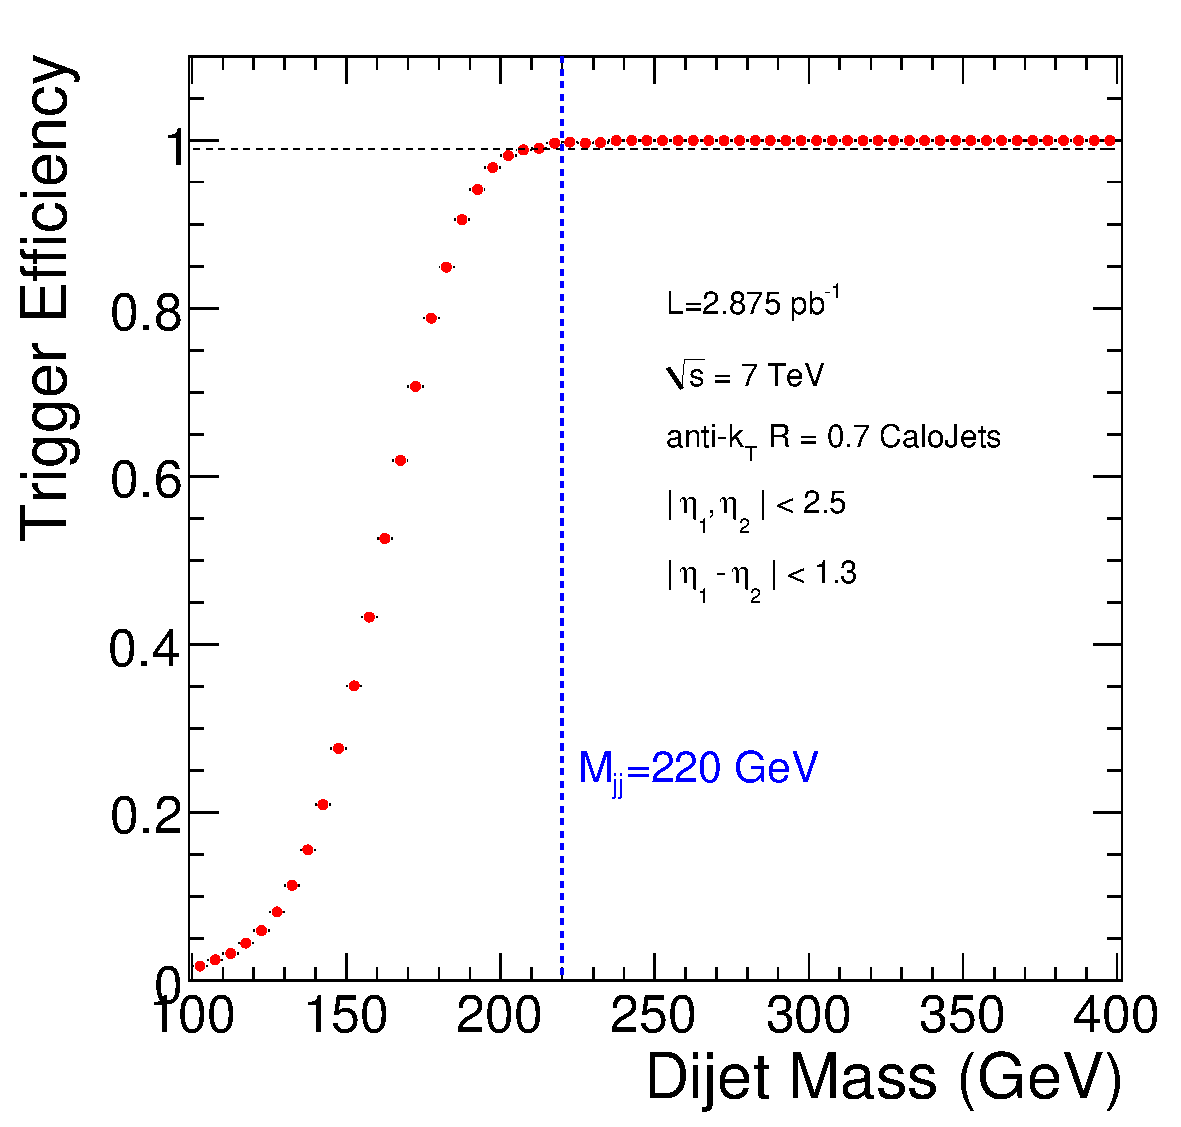
\includegraphics[width=0.6\textwidth]{Figures/HLT_Jet50U.pdf}
    \caption{ HLT\_Jet50U trigger efficiency as a function of dijet mass for 
    $|\eta|<1.3$ is measured from the data.}
    \label{Trigger}
  \end{center}
\end{figure}


The number of events vs. dijet mass are shown in figure~\ref{MassCut}.  The trigger turn over of the 
 HLT\_Jet50U trigger can be seen in the mass spectrum along with the 99\% efficiency ponit at 
 a mass of 210 GeV.  The processed dijet 
cut of 100 GeV has been relaxed to make this plot.

\begin{figure}[!ht]
  \begin{center}
    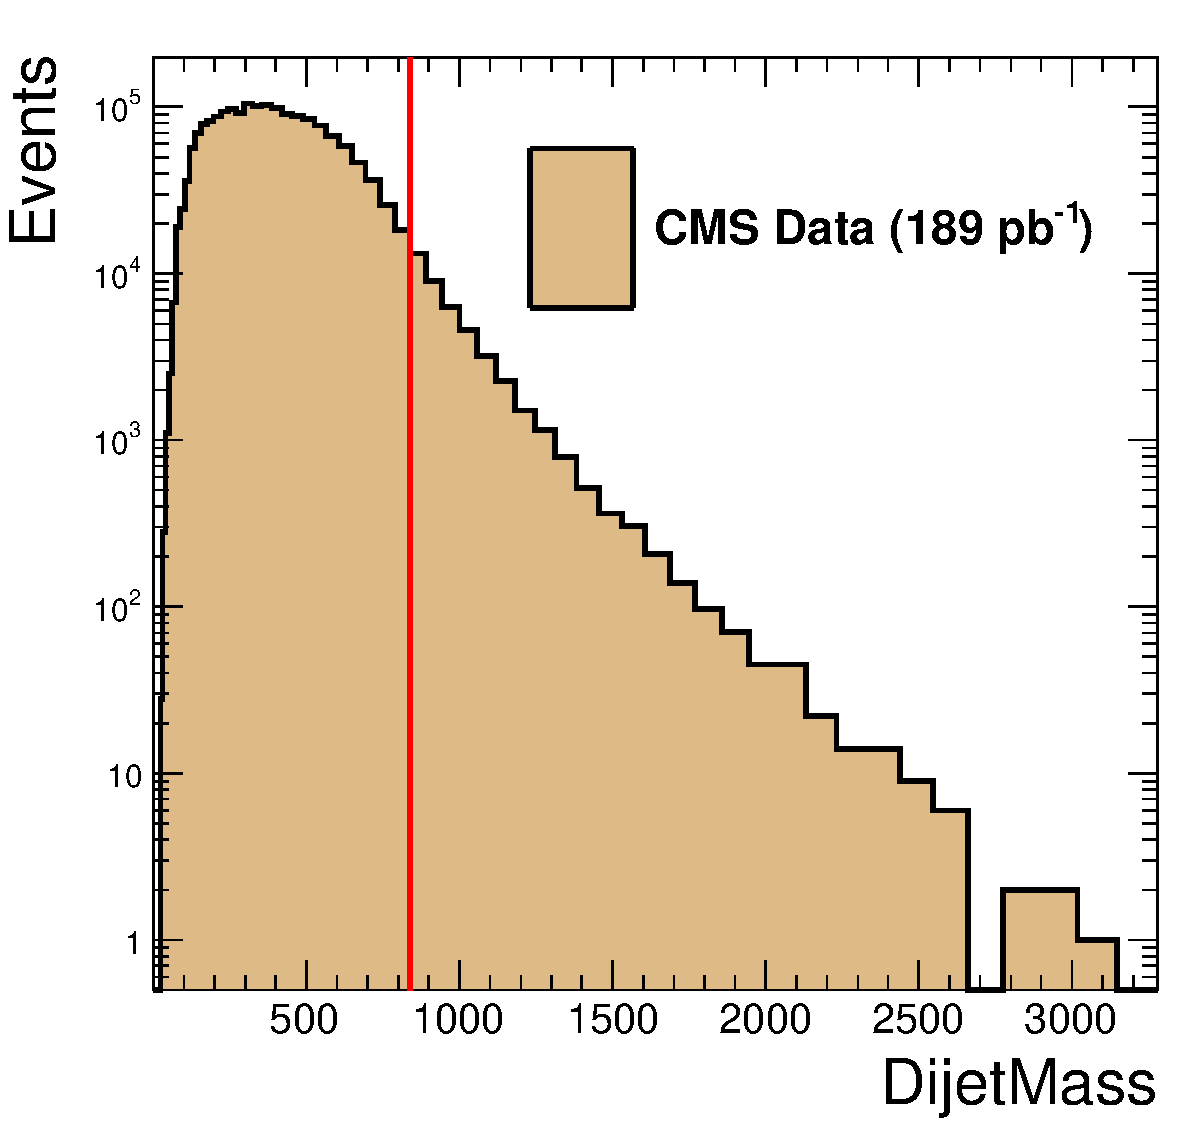
\includegraphics[width=0.6\textwidth]{Figures/c_DijetMass.pdf}
   \caption{ Number of events vs. dijet mass in GeV (histogram) requiring all cuts except the final dijet mass cut for trigger
   efficiency at $m=220$ GeV (vertical line)}
    \label{MassCut}
  \end{center}
\end{figure}
\clearpage
\subsubsection{Dijet Data Quality}

The number of events in the analysis after the basic cuts are shown for
each cut in table~\ref{table:cuts}
\begin{table}[th]
  \centering
  \normalsize
  \begin{tabular}{|l|r|}
    \hline
      Events after vertex cut                              &  6125930\\
      Events after dijet eta cuts: $|\Delta\eta|<1.3$ and $|\eta|<2.5$ & 2088922 \\
      Events after dijet mass cut: $m>200$ GeV & 414645 \\
      Events after jet id cut                              &   414131 \\
    \hline
  \end{tabular}
  \caption{Cuts and Events}
  \label{table:cuts}
\end{table}

The fraction of events rejected by Jet ID is very small, because the requirement that the
two leading jets have a dijet mass $m>220$ GeV, $|\eta|<2.5$ and $|\Delta\eta|<1.3$ enhances the jet purity.
514 events are rejected by jet ID. We have scanned all events rejected by Jet ID that have a dijet
mass of greater than 1.4 TeV, and they are all HPD noise that also has high $MET$, except for one 
event with a Sum $E_T$ of 400 TeV uniformly distributed across the HCAL.
%One event rejected by jet ID (run 139407 event 1102912914) has a jet with EMF of 0.009, but otherwise appears to be a good event with
%a dijet mass of $0.5$ TeV.
%One event rejected by Jet ID was in Event 156365648 in Run 135149, noise in a single RBX giving 
%two neighboring jets with EMF of 0 an event MET/$\Sigma E_T$=0.95. 
%A second event rejected by Jet ID was Event 217914565 in Run 135528, noise in  a single HPD,
%again giving two neighboring jets with EMF of 0 and fHPD of 1 and an event MET/$\Sigma E_T$=0.87.
%A third event rejected by Jet ID was Event 103871079 in Run 135175, in which the leading jet
%failed the EMF cut with $EMF=0.005$, but the event looks like it might be a real dijet event:
%jet 1 $p_T=74$ GeV, jet 2 $p_T=35$ GeV, $M_{JJ}=156.4$ GeV, tracks pointing at both jets, 
%$\Delta\phi=2.7$, and a marginal but passable MET/$\Sigma E_T$=0.24.  


After all cuts, we present some basic distributions indicating jet and event quality in 
Fig.~\ref{jet_id}, ~\ref{basic_event} and ~\ref{jet_kinematics}.


In Fig.~\ref{jet_id} we show the distributions of the variables of loose jet ID
after all cuts.  Jet EMF, the fraction 
of jet energy in the ECAL, does not have a peak near either zero or one which would indicate a 
problem from the
HCAL or ECAL. Loose jet ID requires jet EMF$ > 0.01$ and we find
that the cut rejects no real jets in dijet events as discussed above. Jet fHPD, the fraction of jet energy in 
the hottest HCAL HPD, does not have a peak near one which would indicate a problem from 
HPD noise.  Loose jet ID requires
jet fHPD$ < 0.98$.  Jet n90hits, the number of energy ordered HCAL and ECAL RecHits 
containing 90\% of the jet energy, does not have a peak near one which would indicate 
hot cells in the calorimeter for example from Ecal spikes.
Loose jet ID requires jet n90hits $> 0$.  Data and MC have
similar shapes and show smoothly 
varying distributions for jet EMF, fHPD, and n90hits 
characteristic of real jets.  These jet ID variables give us confidence 
that the jets in this analysis do not originate from backgrounds in the calorimeter.

In Fig.~\ref{track_multiplicity} we show the number of good tracks 
associated with either of the two leading jets.  Our leading jets generally have many 
associated tracks.  Very few of the leading jets, in both MC and data, have no 
associated tracks at the calo face, and there are virtually no leading jets without associated
tracks at the vertex. The track multiplicity distributions do not have a peak at zero tracks,
which would indicate calorimeter backgrounds.  The track multiplicity distribution gives 
us additional confidence that the calorimeter jets in this analysis come from pp collisions.

In Fig.~\ref{basic_event} we show some event balance distributions.  
The dijet events have low MET/$\Sigma E_T$,
the ratio of the magnitude of the vector and scalar sums of the CaloTowers,
indicating that the event energy is well balanced in the transverse plane. 
Large background from calorimeter noise, beam halo, or cosmic rays will typically
produced large values of MET/$\Sigma E_T$, which we do not observe in this data.
The handful of events with MET/$\Sigma E_T>0.5$ have been scanned, and they all look like good 
monojet events at dijet mass around $0.2-0.3$ TeV, most likely from 
$W(\mu \nu)$ + jet or $Z(\mu\mu, \nu\nu)$ + jet processes.
The two leading jets are predominantly back-to-back in $\phi$ as expected for 
dijets, with a tail to small values of $\Delta\phi$ produced by radiation 
and multi-jet events. 
Data and MC have similar shapes and show 
smoothly varying distributions for  MET/$\Sigma E_T$ and $\Delta\phi$ 
characteristic of dijet events. Thes distributions give us confidence
that we are observing events with a dijet topology, not unphysical backgrounds.


In Fig.~\ref{jet_kinematics} we show some distributions of basic jet
kinematic variables.  The $p_T$ distribution falls steeply with increasing
$p_T$, and turns over at low $p_T$ due to the dijet mass cut $m>354$ GeV.
The jet $p_T$ distributions for data and MC are in good agreement considering
uncertainties in the jet energy scale, discussed in section~\ref{JESerror}, 
and the modelling of the $p_T$ distribution
in PYTHIA.
The $\eta$ distribution of the two leading jets is in reasonable agreement with 
the shape predicted by the MC, and there are no regions with significant
rate deviations that could arise due to significant mis-understanding of jet response
after all corrections. The $\Delta\eta$ distribution demonstrates the 
characteristic forward peaks from Rutherford-like QCD scattering at 
fixed invariant mass, and the very slight deviations in shape between
data and MC are expected from NLO effects on the angular distribution.
The $\phi$ distribution of the two leading jets is flat, with an RMS of
only 2.2\%, which corresonds to a CaloJet response which is flat as a function of phi 
to within about 0.4\%, which is reasonable given expected calorimeter response uniformity in $\phi$. 
The $\eta$ - $\phi$ distribution of two leading jets is reasonably uniform and 
does not show any indication of hot or dead regions of the calorimeter. 
These distributions show that the jets in this data sample 
have the kinematics expected for dijets from QCD.

\begin{figure}[!ht]
  \begin{center}
    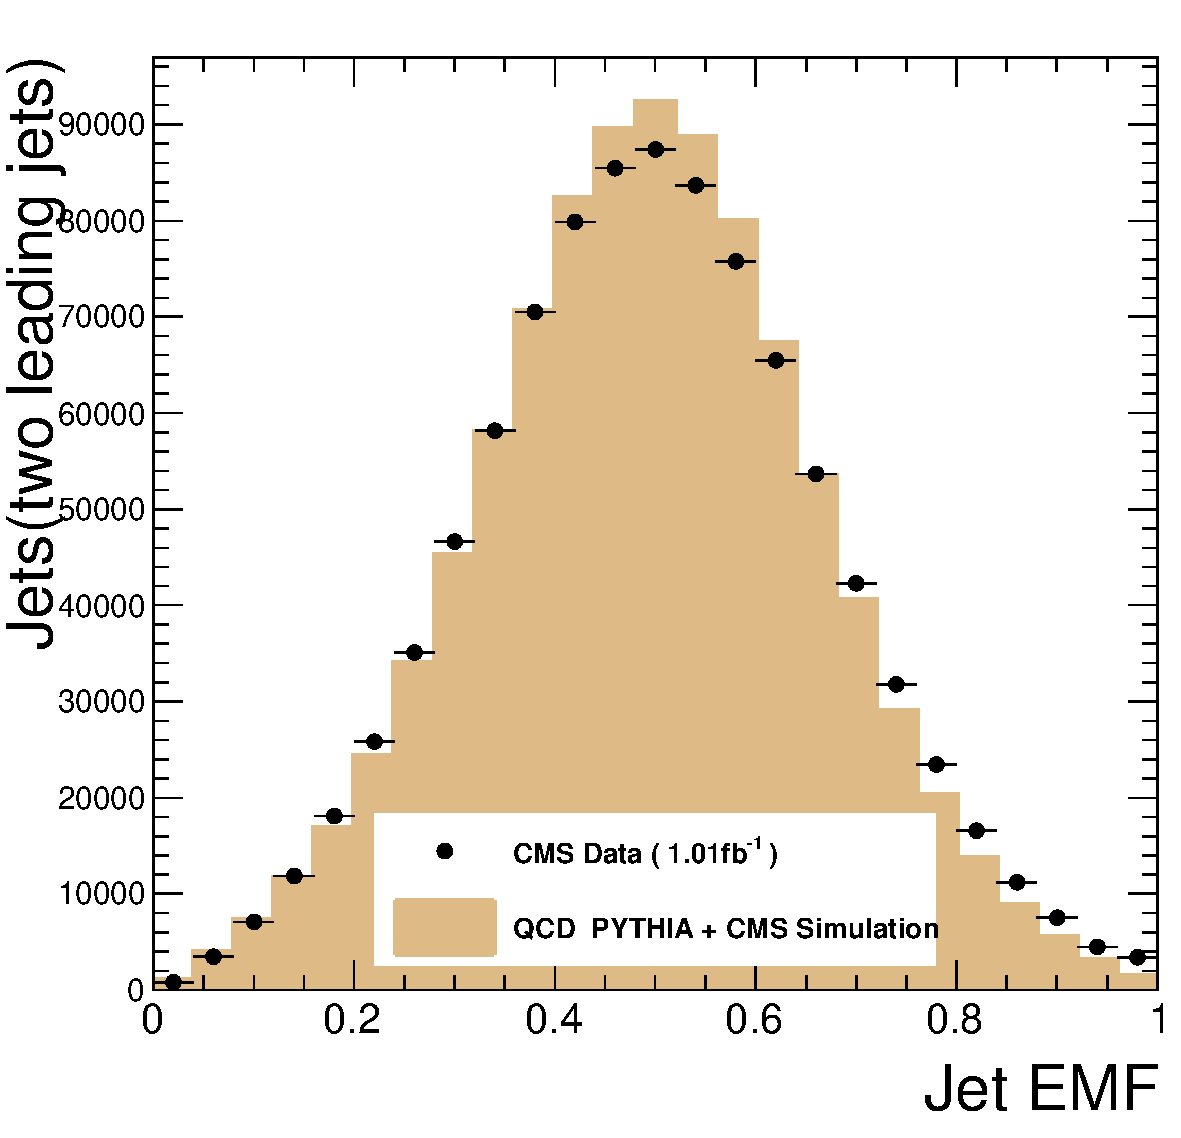
\includegraphics[width=0.45\textwidth]{Figures/c_EMF.pdf}
    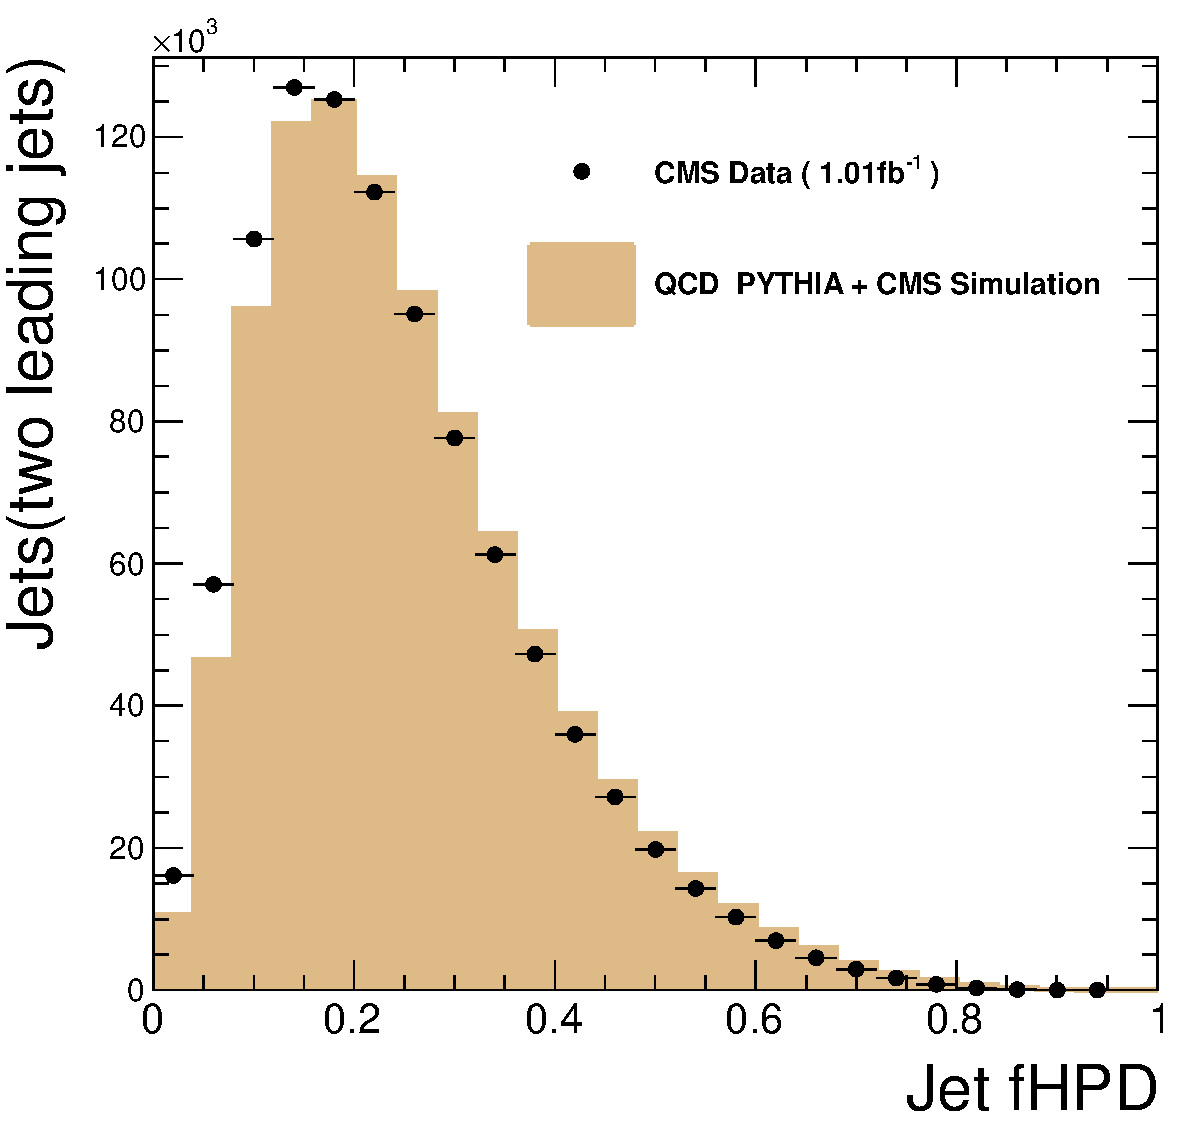
\includegraphics[width=0.45\textwidth]{Figures/c_fHPD.pdf}
    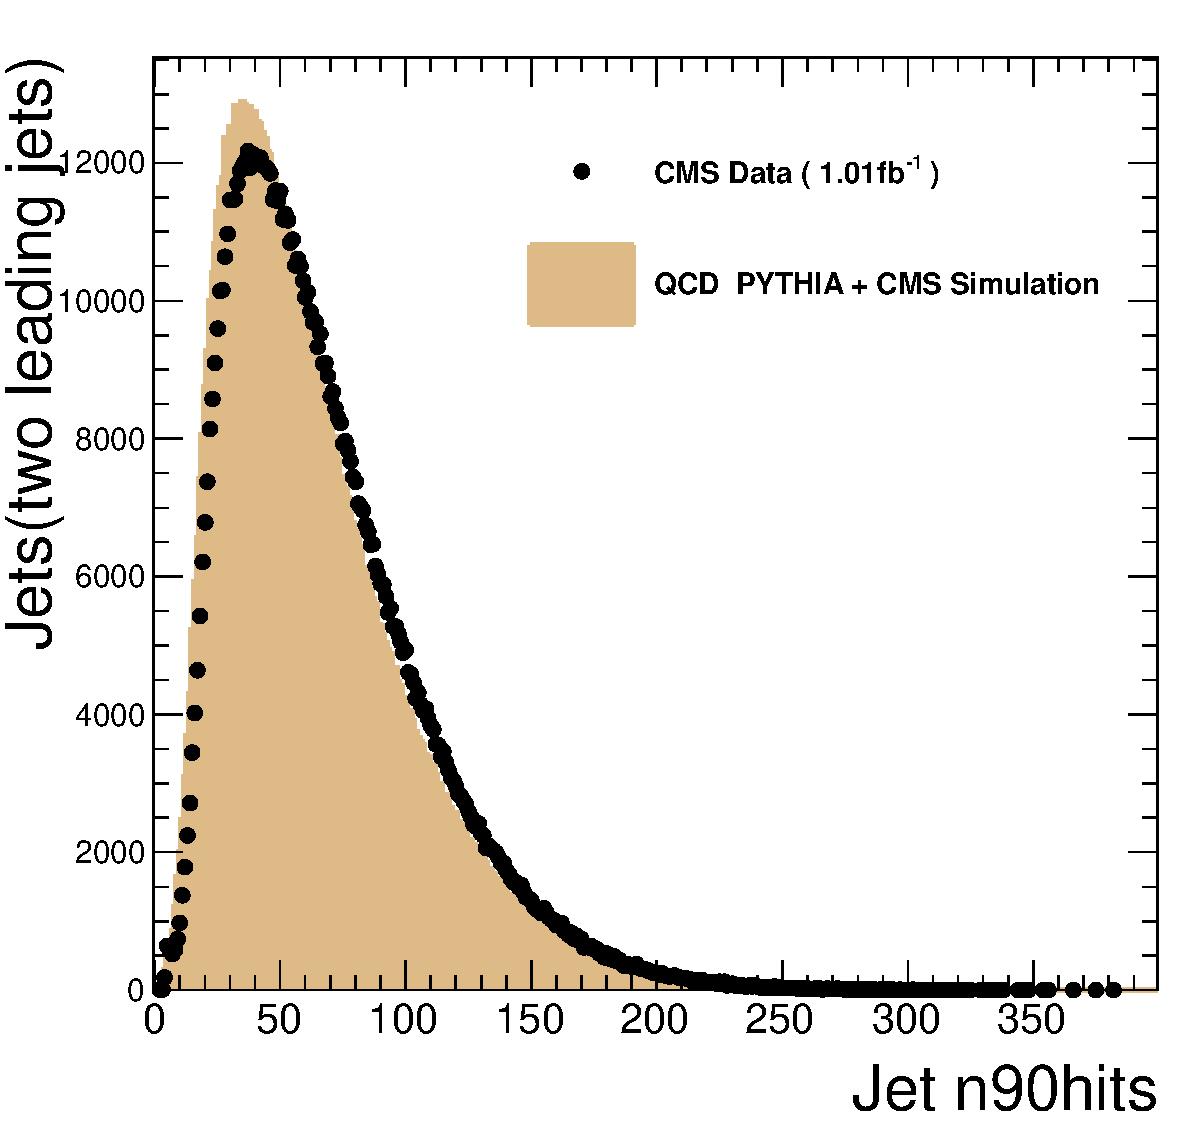
\includegraphics[width=0.45\textwidth]{Figures/c_n90hits.pdf}
    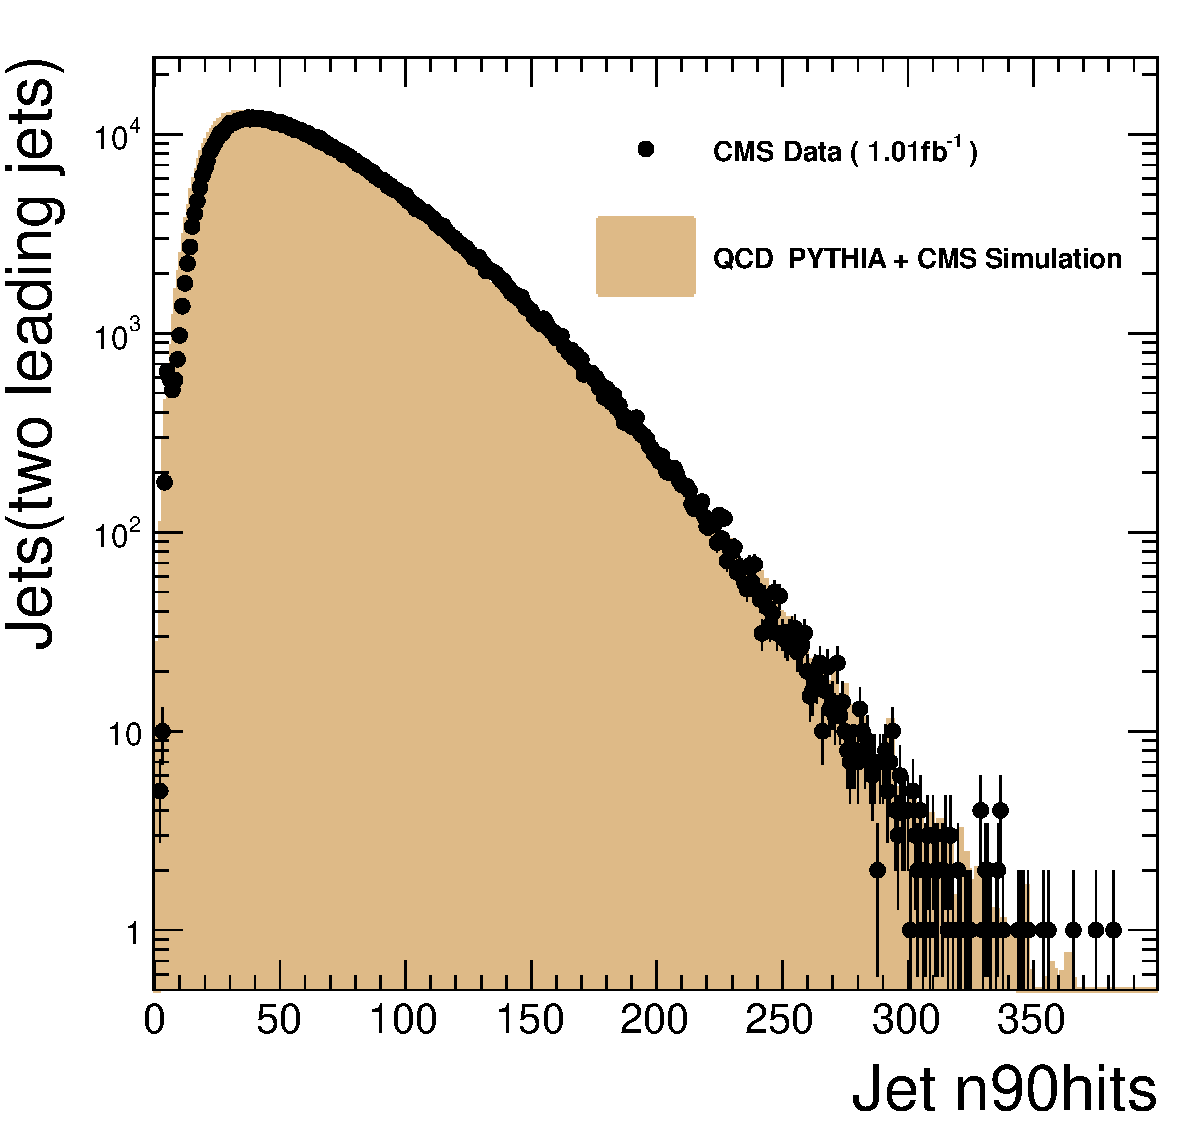
\includegraphics[width=0.45\textwidth]{Figures/c_n90hits_log.pdf}

    \caption{Jet ID Distributions.  The EM
      energy fraction of the two leading jets (upper left), the fHPD for the two
      leading jets (upper right), the n90hits for the two leading jets
      (lower left) and the same in log scale
      (lower right). }
    \label{jet_id}
  \end{center}
\end{figure}

\begin{figure}[!ht]
  \begin{center}
    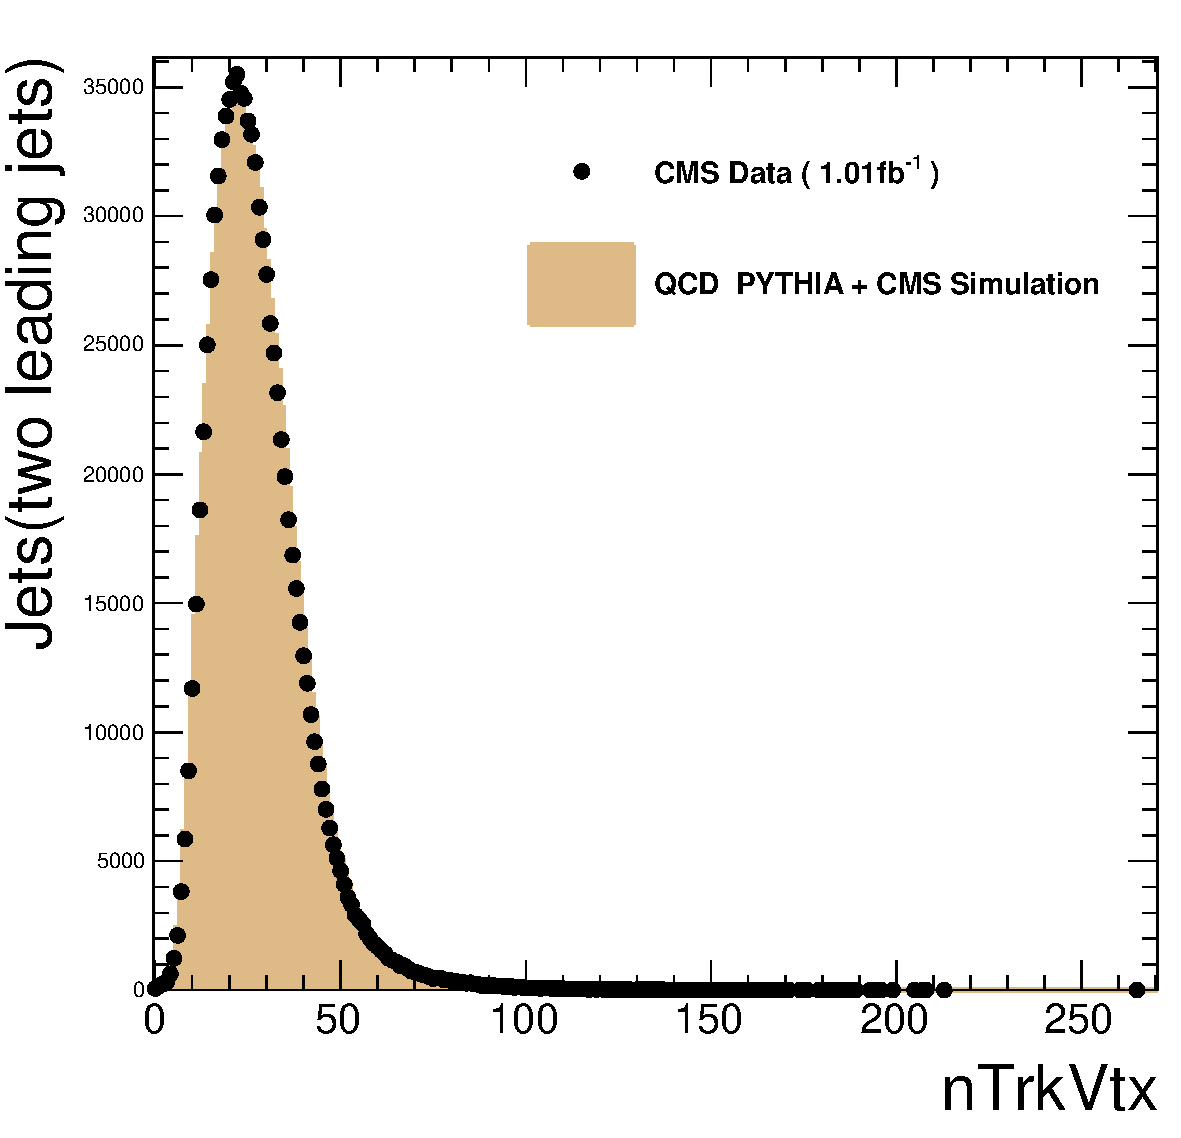
\includegraphics[width=0.45\textwidth]{Figures/c_nTrkVtx.pdf}
    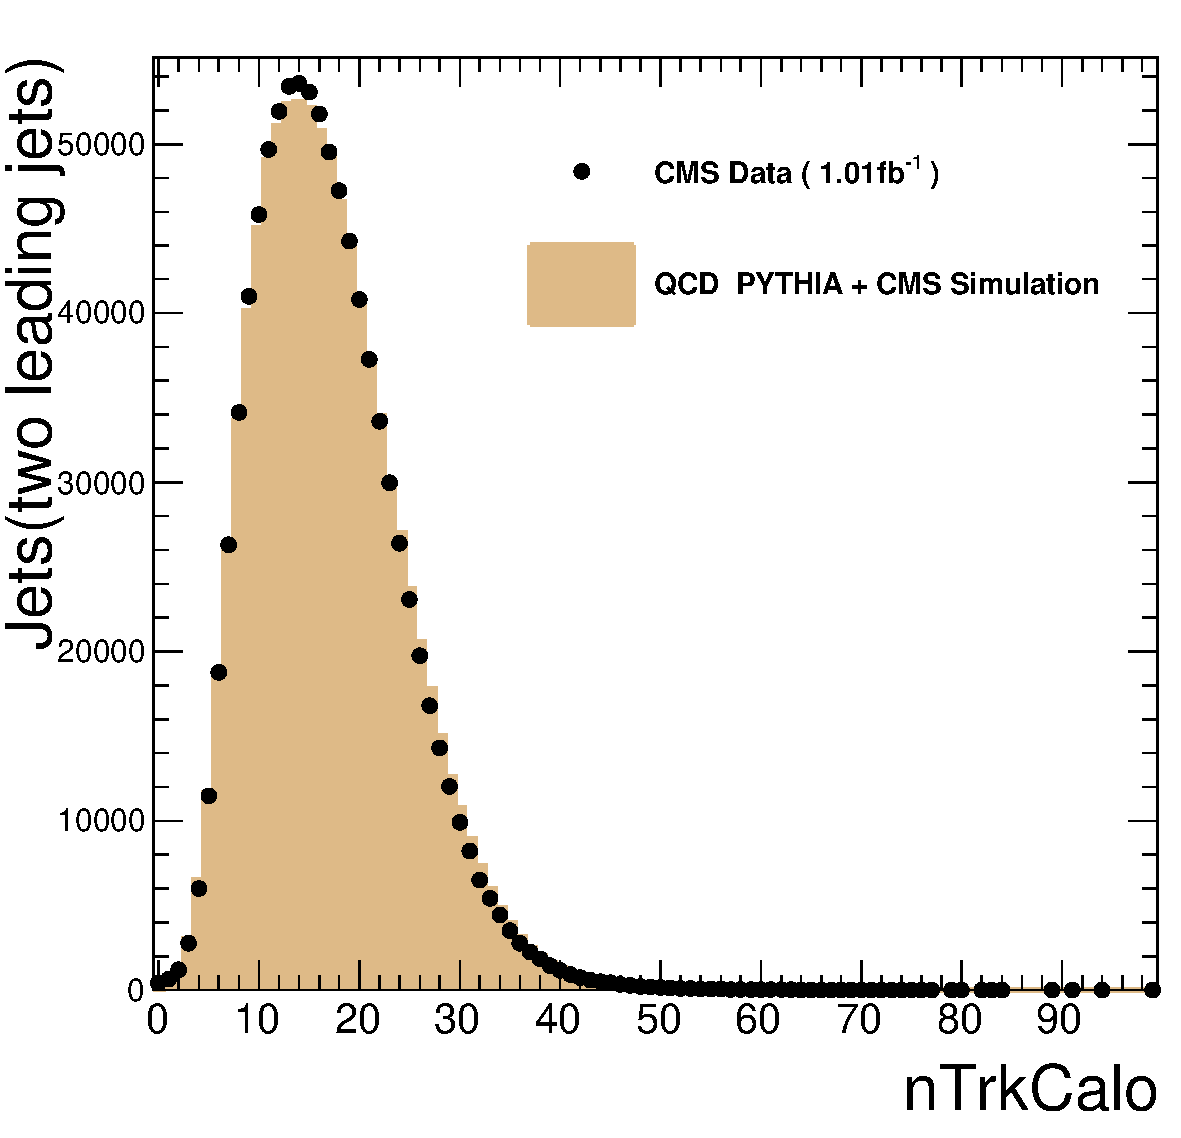
\includegraphics[width=0.45\textwidth]{Figures/c_nTrkCalo.pdf}
    \caption{ left) The multiplicity of tracks associated to two leading jets at the vertex right) The multiplicity of tracks associated to two leading jets at the calo face}
    \label{track_multiplicity}
  \end{center}
\end{figure}

\begin{figure}[!ht]
  \begin{center}
   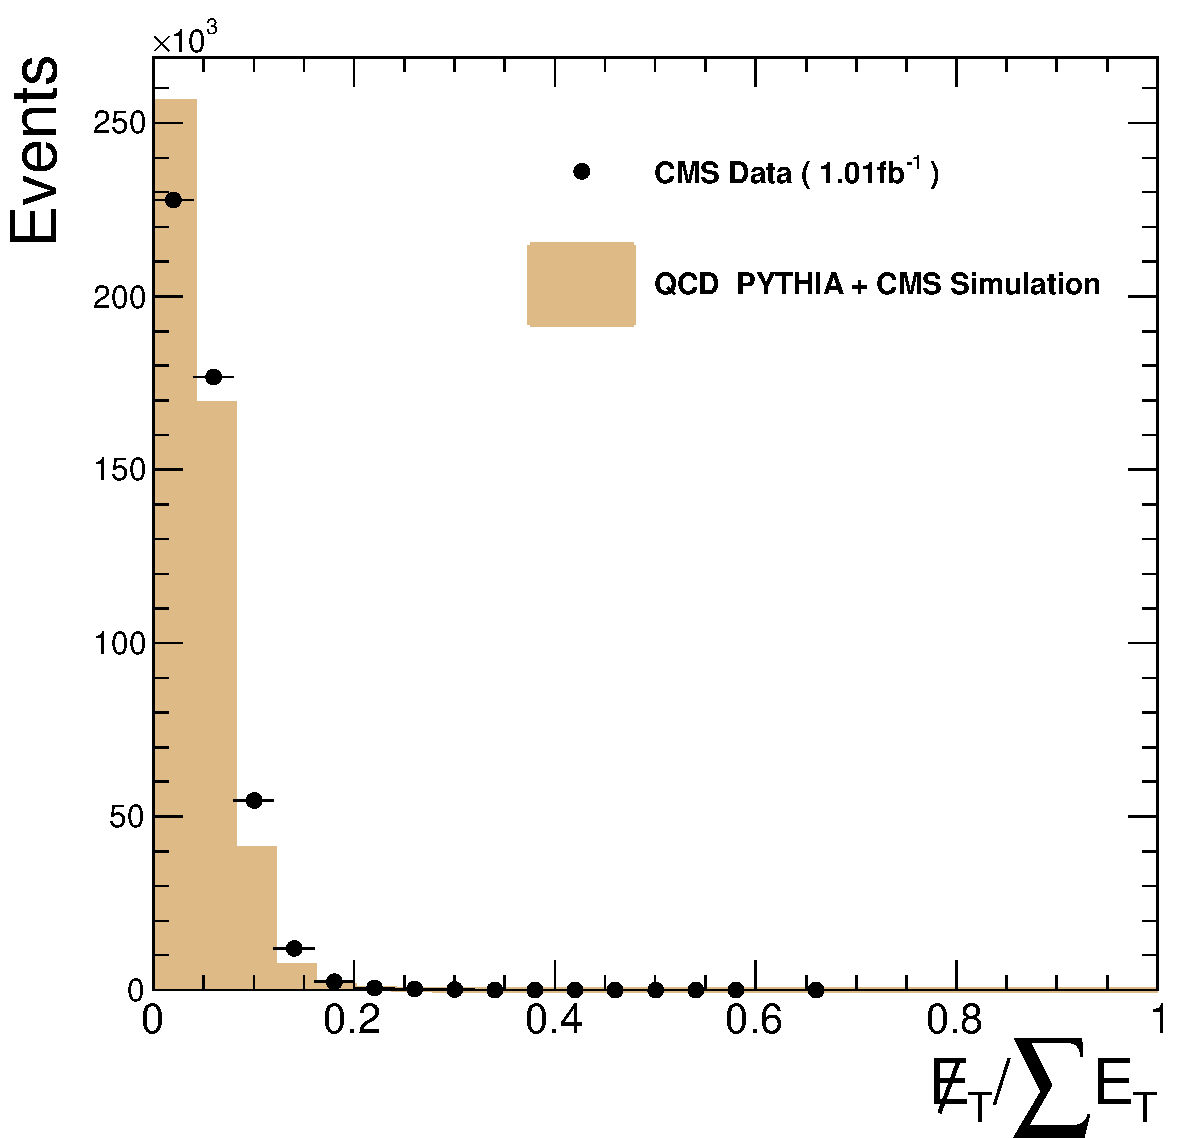
\includegraphics[width=0.45\textwidth]{Figures/c_MET_over_sumEt.pdf}
   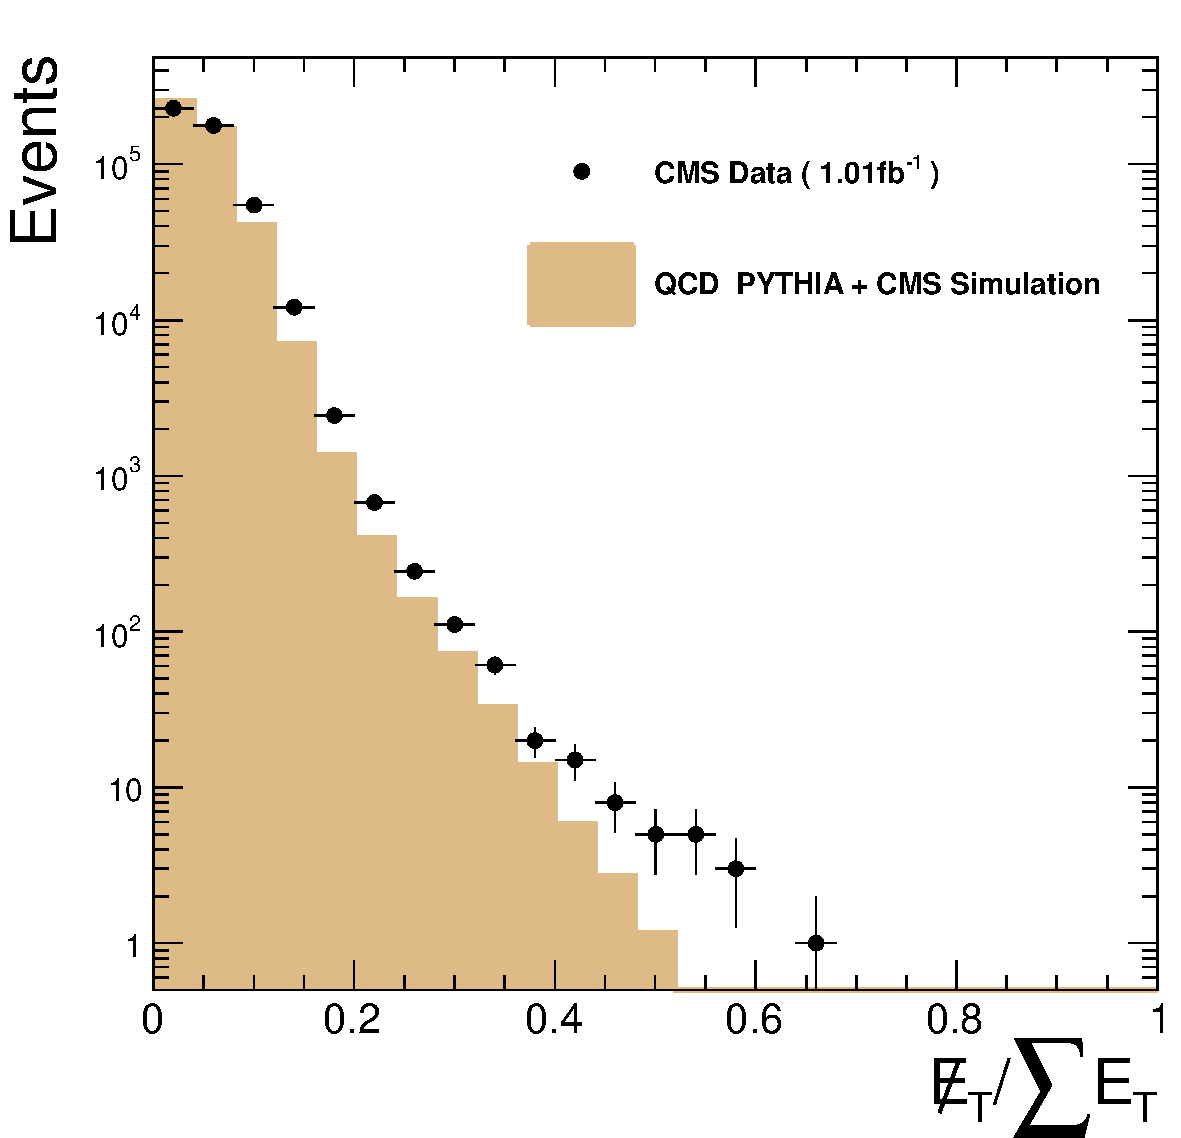
\includegraphics[width=0.45\textwidth]{Figures/c_MET_over_sumEt_log.pdf}
   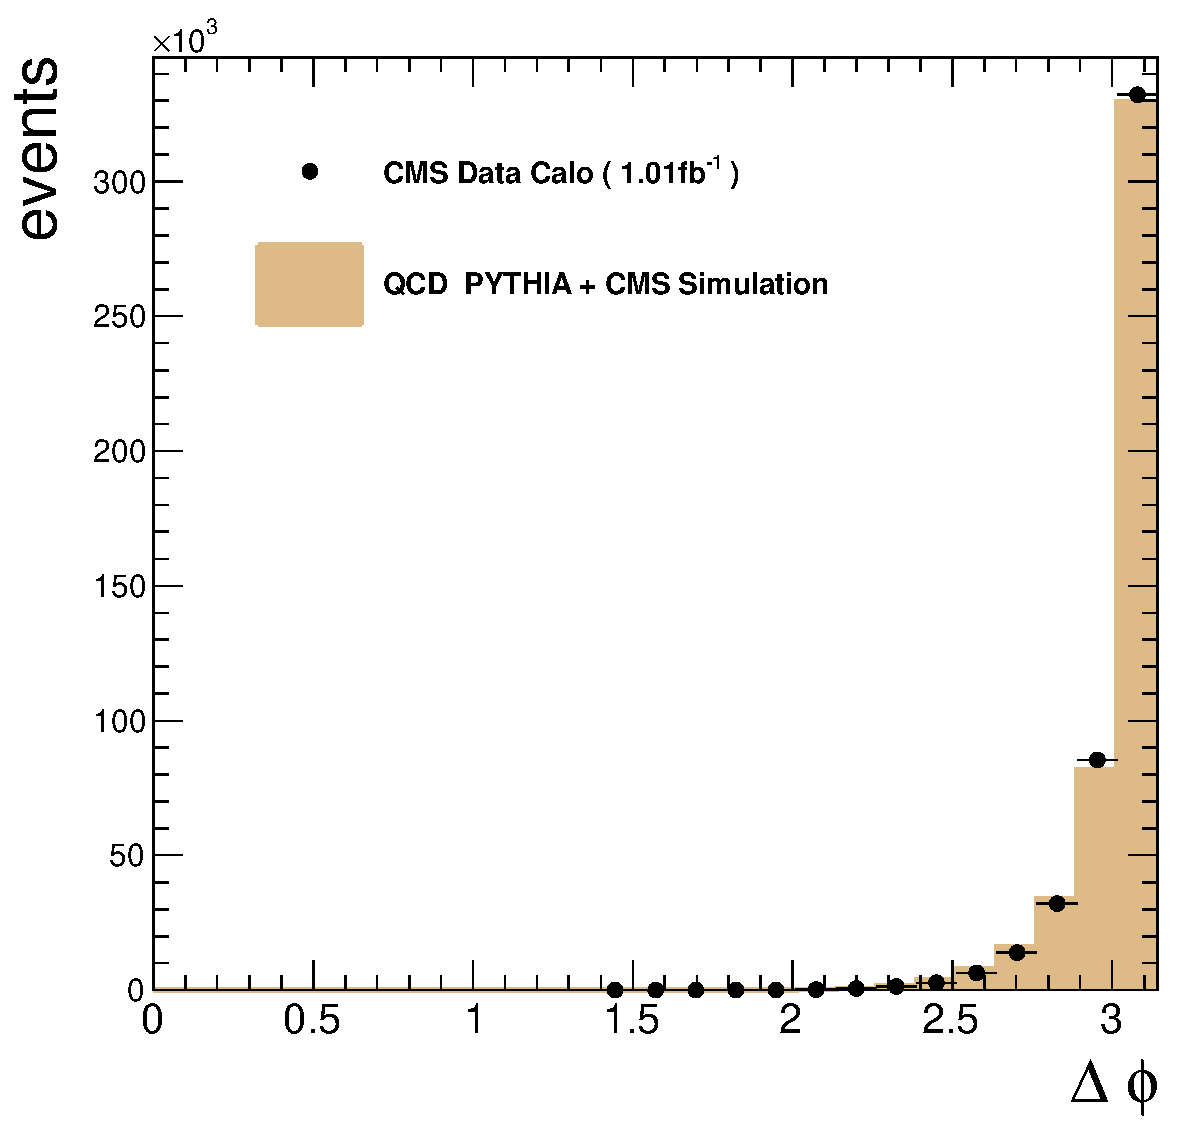
\includegraphics[width=0.45\textwidth]{Figures/c_DPhi.pdf}
   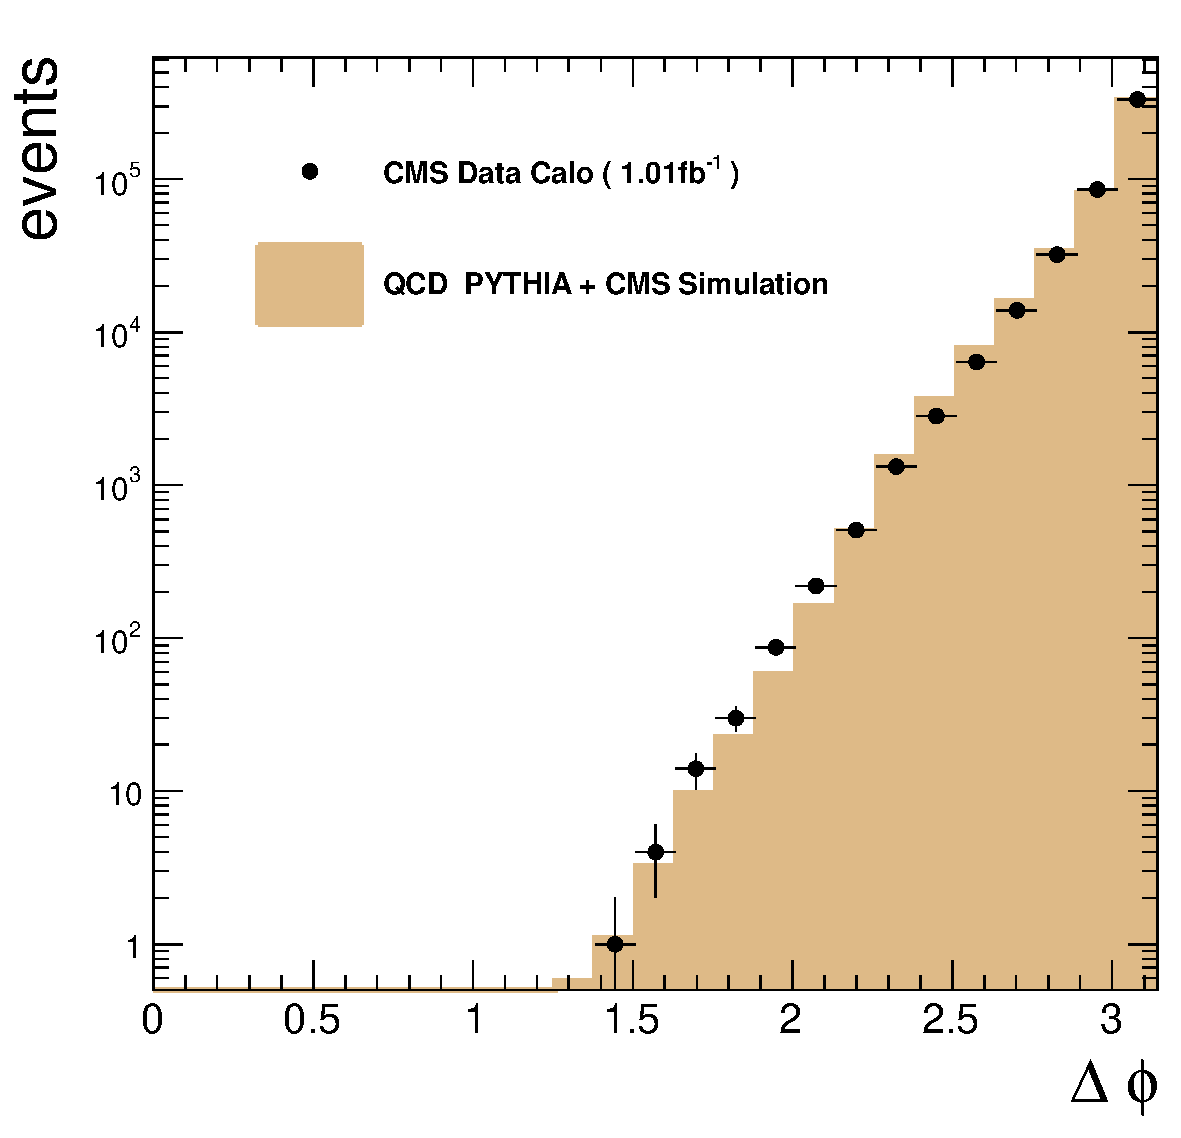
\includegraphics[width=0.45\textwidth]{Figures/c_DPhi_log.pdf}

   \caption{ Event balance distributions.  Missing
    calorimeter $E_T$ divided by total calorimeter $E_T$ 
    (upper left) and the same in log scale (upper right).
    The $\phi$ difference of the two leading jets (lower left) 
    and the same in log scale (lower right).}
    \label{basic_event}
  \end{center}
\end{figure}


\begin{figure}[!ht]
  \begin{center}
    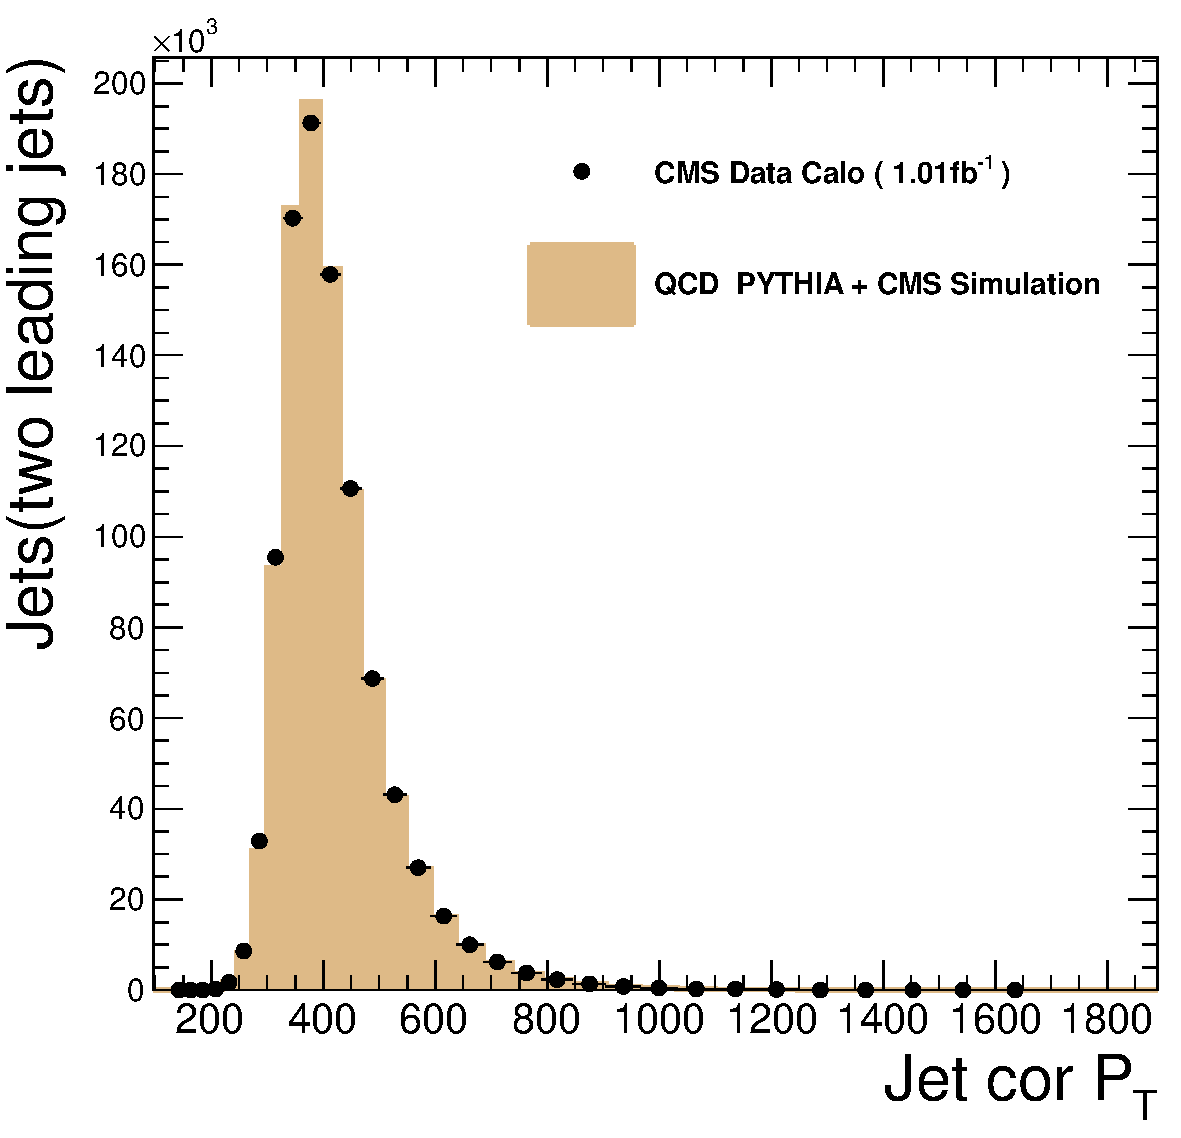
\includegraphics[width=0.45\textwidth]{Figures/c_corPt.pdf}
    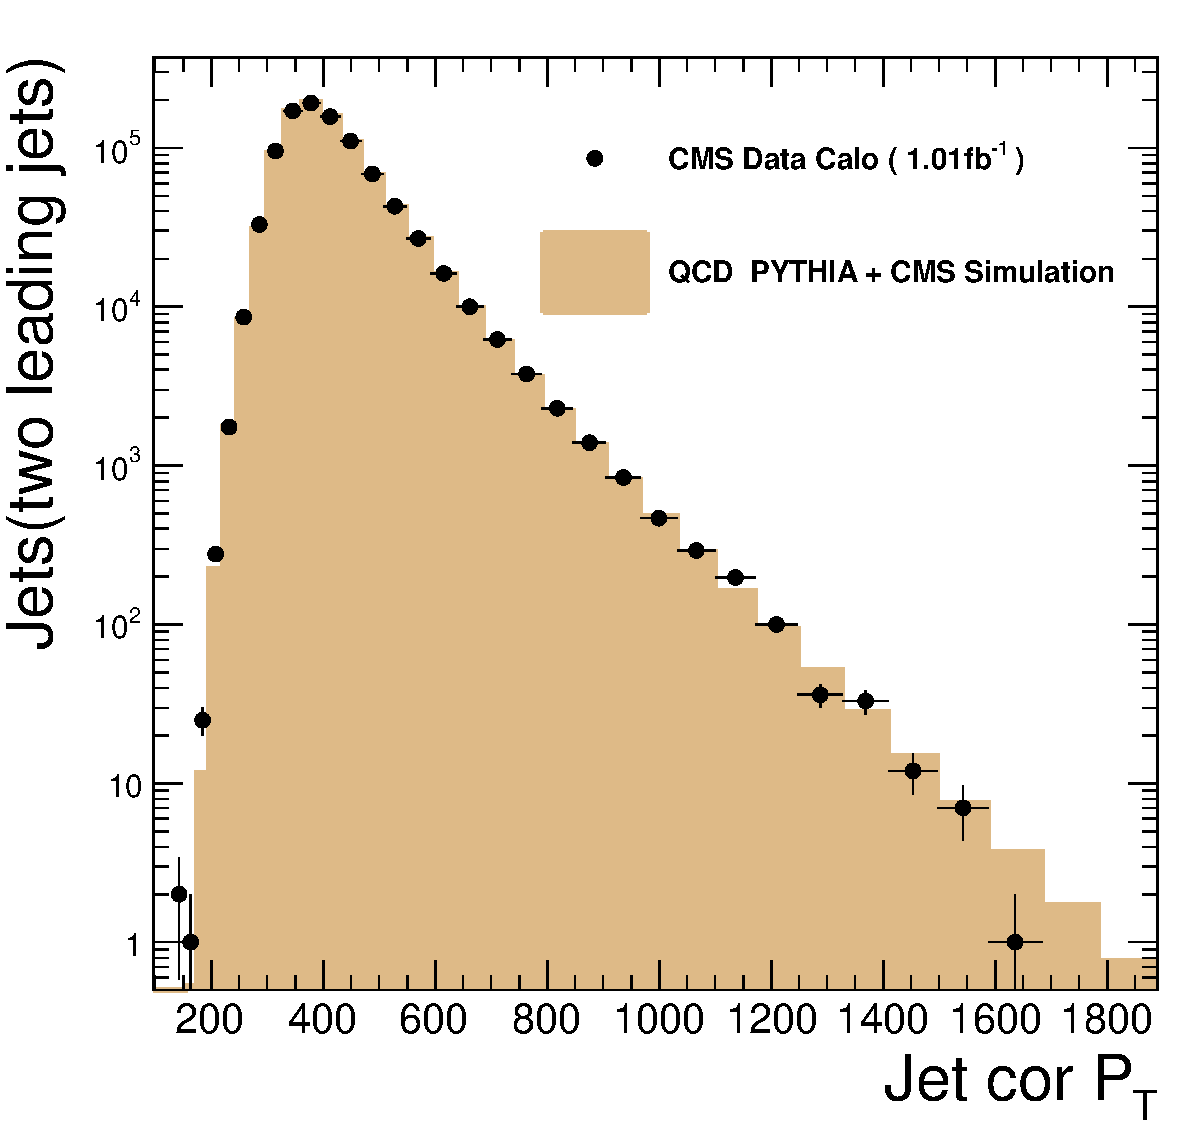
\includegraphics[width=0.45\textwidth]{Figures/c_corPt_log.pdf}
    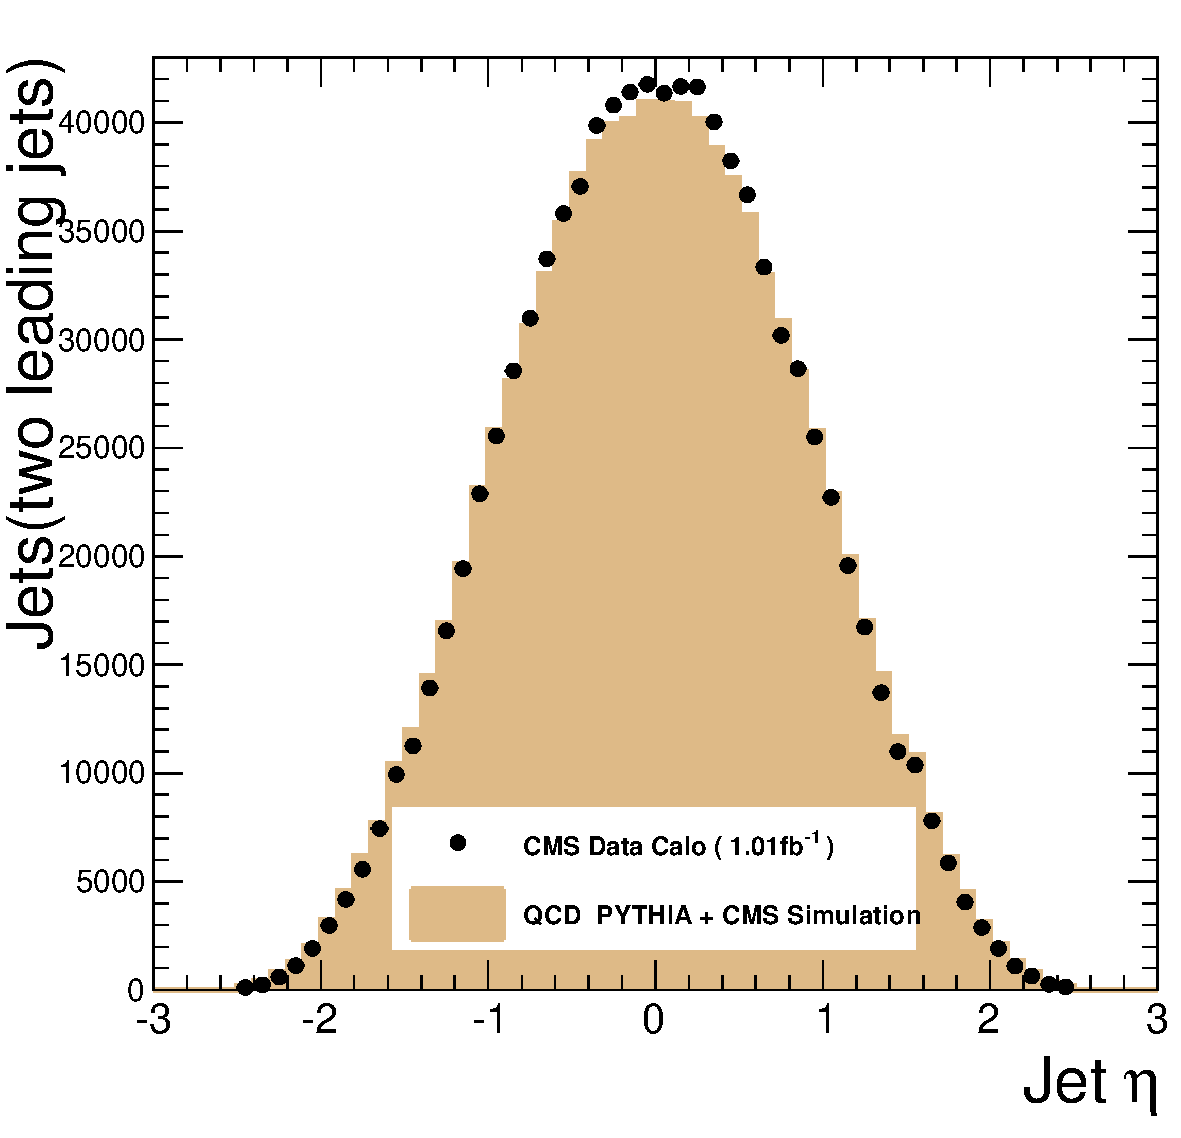
\includegraphics[width=0.45\textwidth]{Figures/c_Eta.pdf}
    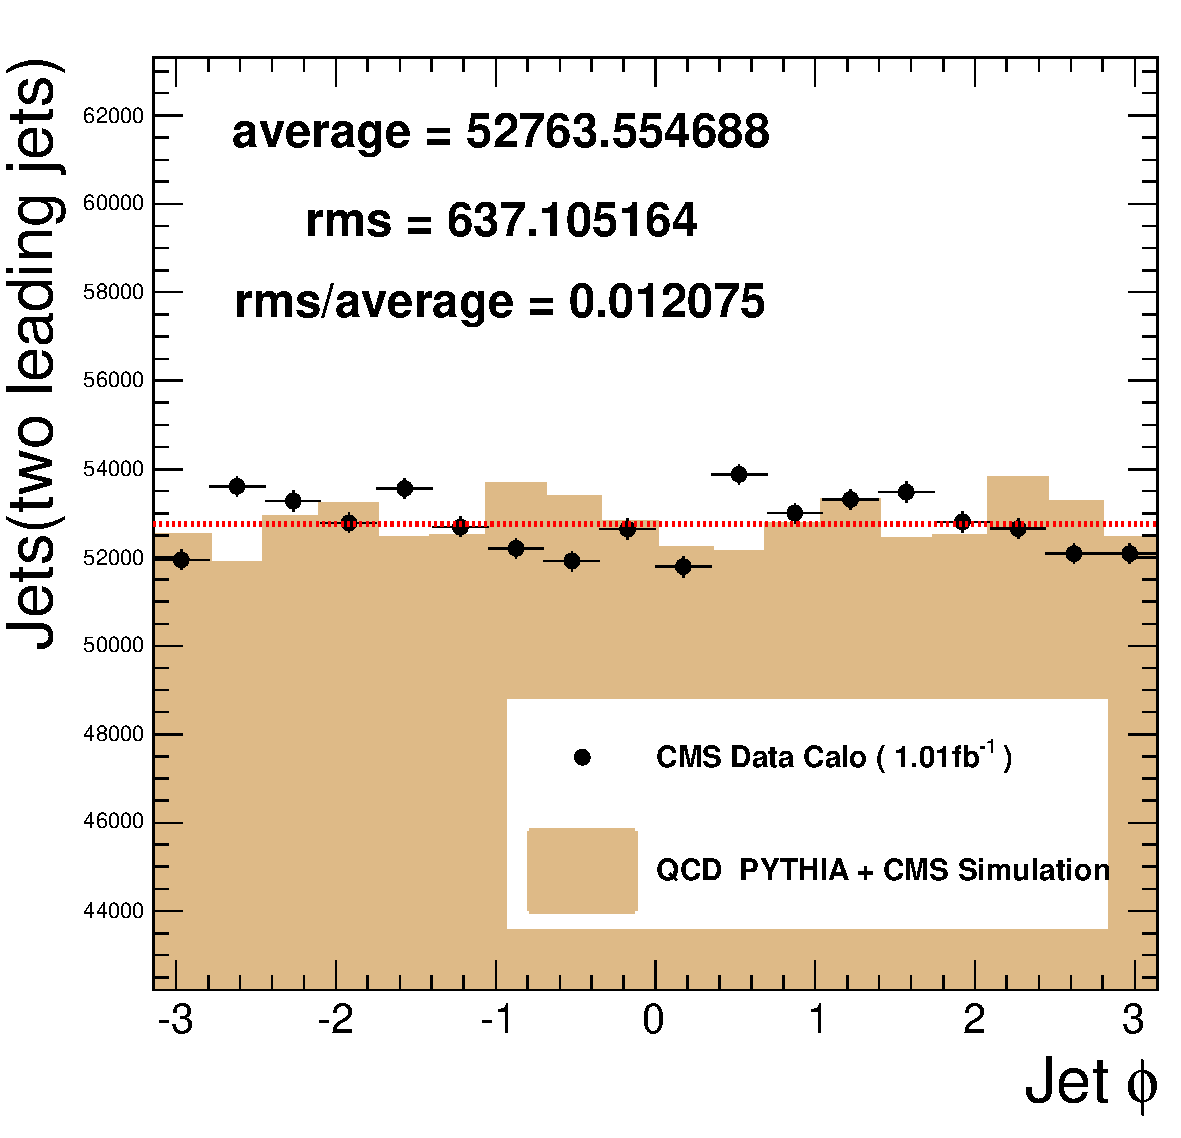
\includegraphics[width=0.45\textwidth]{Figures/c_Phi.pdf}
    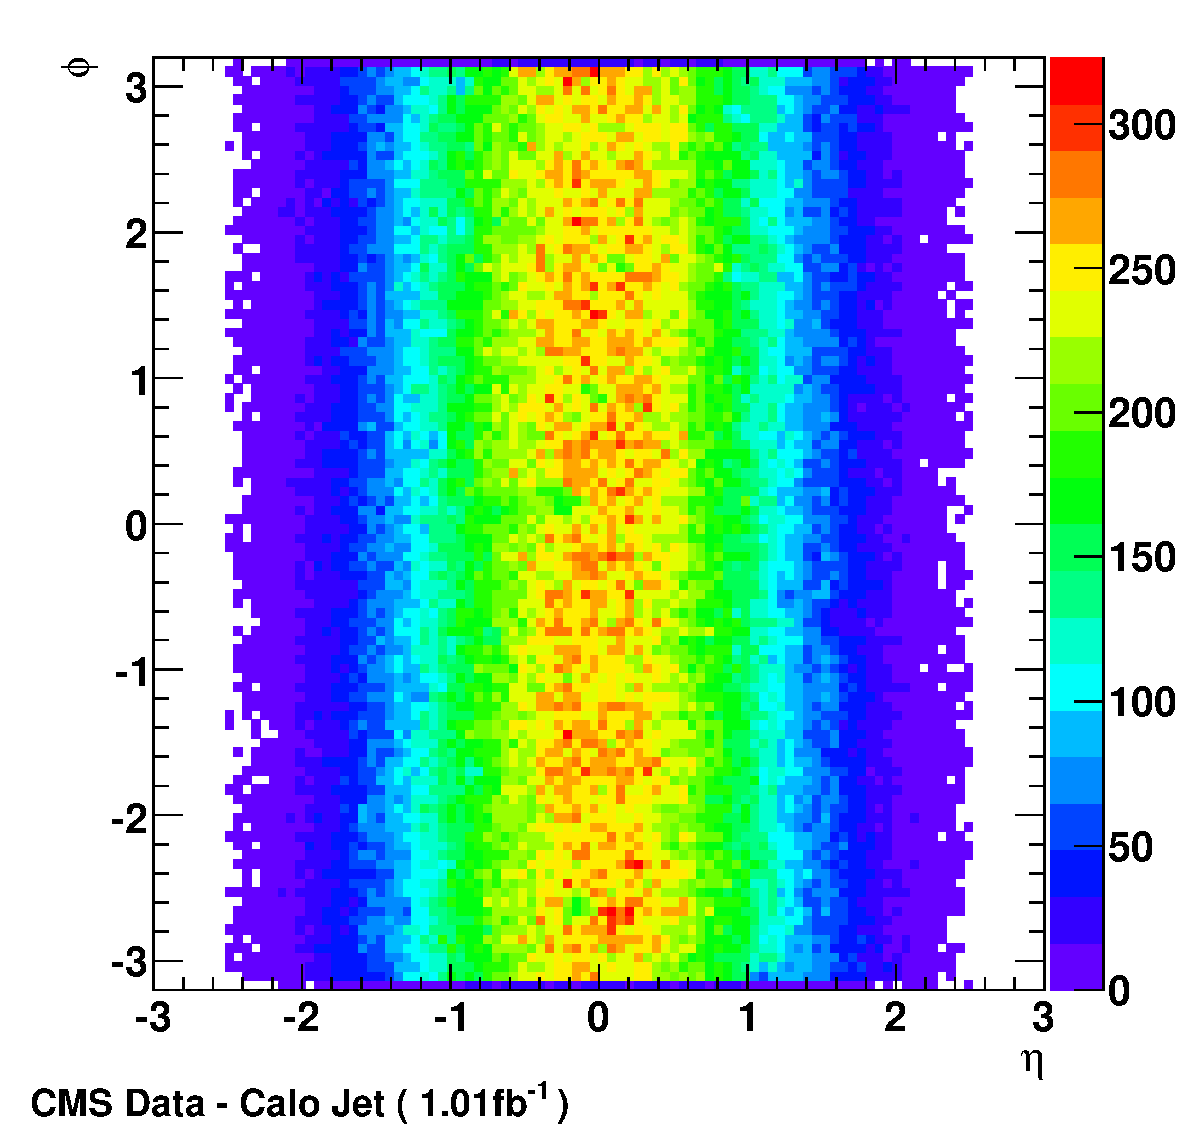
\includegraphics[width=0.45\textwidth]{Figures/c_Eta_Phi_Scatter.pdf}
    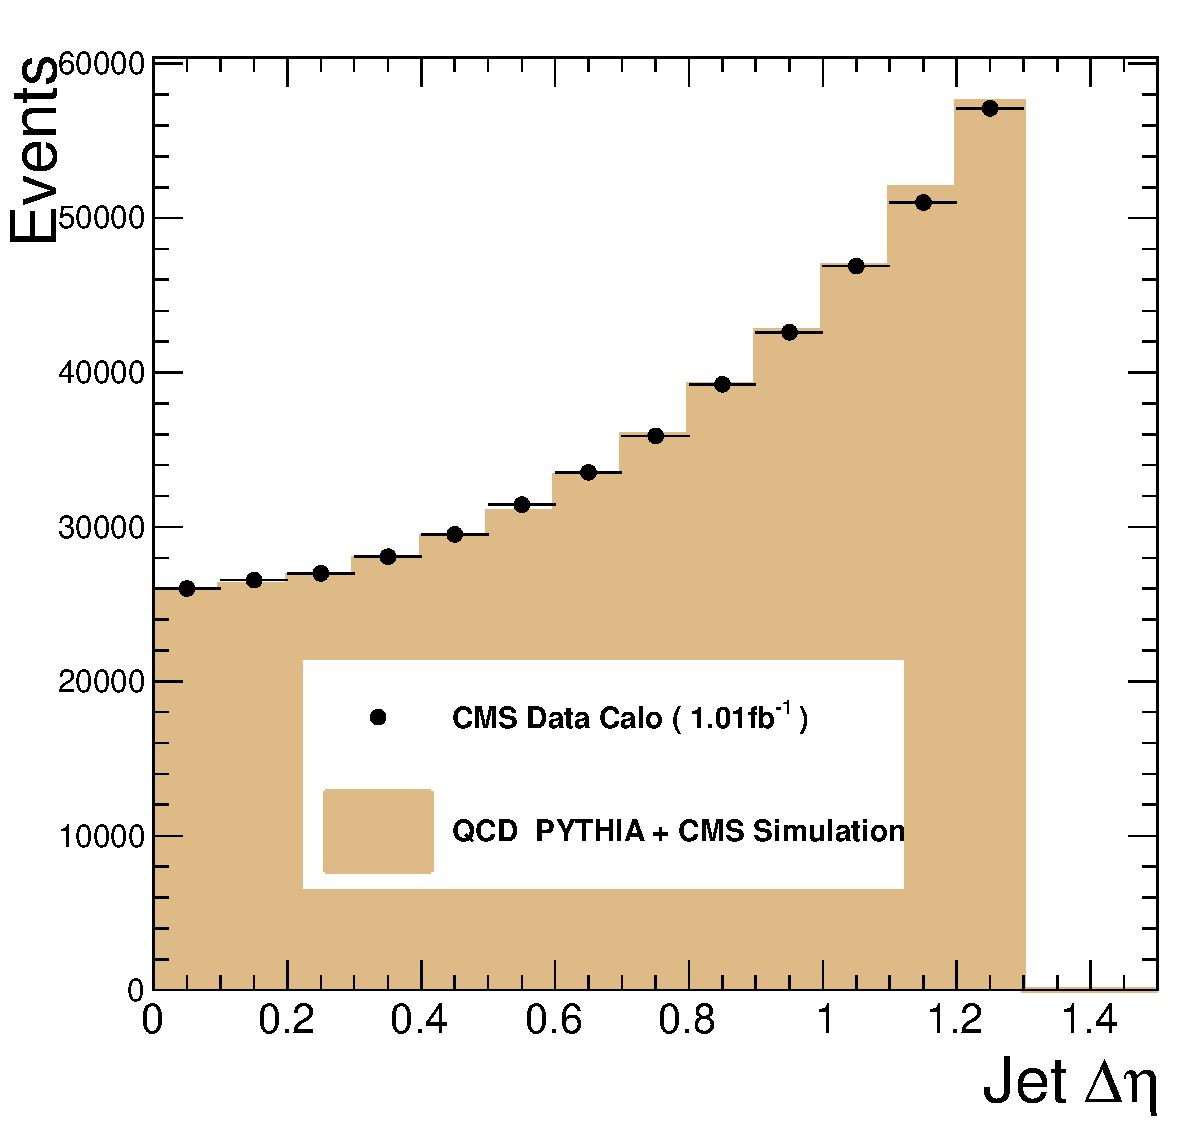
\includegraphics[width=0.45\textwidth]{Figures/c_DEta.pdf}

    \caption{ Jet kinematics distributions.  The corrected 
      $P_T$ of the two leading jets (upper left) and the same in log scale
      (upper right). The $\eta$ distribution for the
      two leading jets (middle left). The $\phi$ distribution for the two leading jets. (middle right)
      $\phi$ vs. $\eta$ (lower left) for the two leading jets. The $\Delta\eta$ distribution (lower right) }
    \label{jet_kinematics}
  \end{center}
\end{figure}


\subsubsection{Dijet Data Stability}

In order to demonstrate the stability of our data as a function of run, we show various event
and jet related quantities. In Fig.~\ref{MassVsRun} we show the number of dijet events surviving 
the full selection, for each run used in the analysis. We also show the mean dijet mass vs. run. 
In Fig.~\ref{XsecVsRun}, we show the number of dijet events divided by the integrated luminosity
of each run, vs. run. The observed cross-section is well behaved and very stable with an RMS of 
only 2\%.
%, with $\sim 20\%$ fluctuation around
%the weighted average primarily due to low number of events per run; 
A minimum
luminosity of 1 nb$^{-1}$ in each 
run is required for the plot. The cross-section as a function of run is  very 
sensitive to the jet energy scale stability which in turn is sensitive to the 
the calibration of the calorimeter. A change of just 0.4\% in the jet energy scale between
one run and the next would produce a change of around 2\% in the observed cross
section.  In addition, the cross-section is sensitive to the luminosity 
evaluation.  The observed stability of the cross section is an indication of a stable calorimeter energy 
scale and luminosity evaluation.

In Fig.~\ref{JetPropertiesVsRun} we show the mean value of the basic jet properties (\pt, EMF, number of
associated tracks), separately for the two leading jets, vs. run. Good stability is observed for all observables.

\begin{figure}[!ht]
  \begin{center}
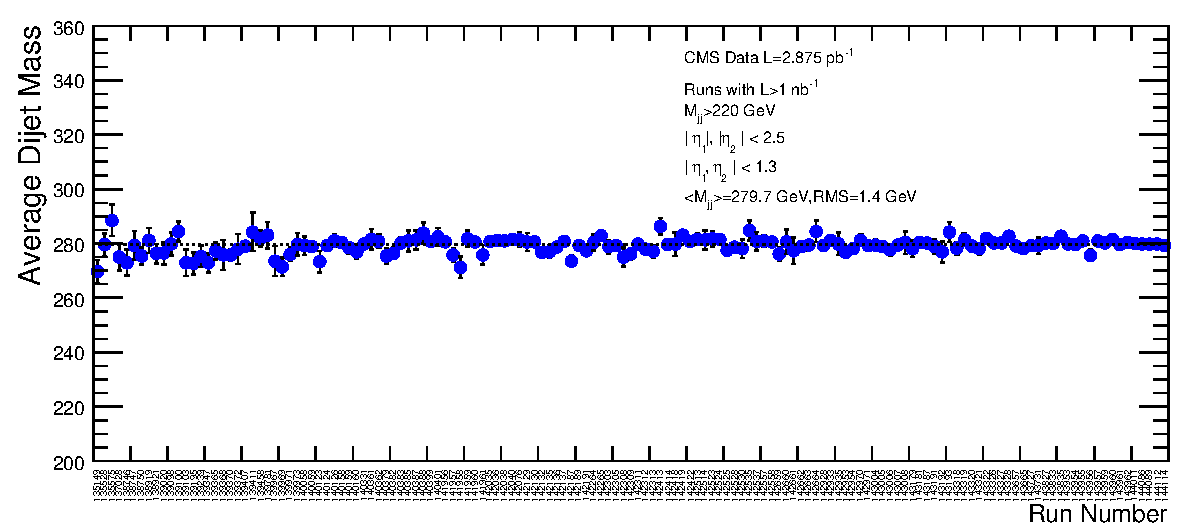
\includegraphics[width=0.9\textwidth]{Figures/MassVsRunNo.pdf} 
%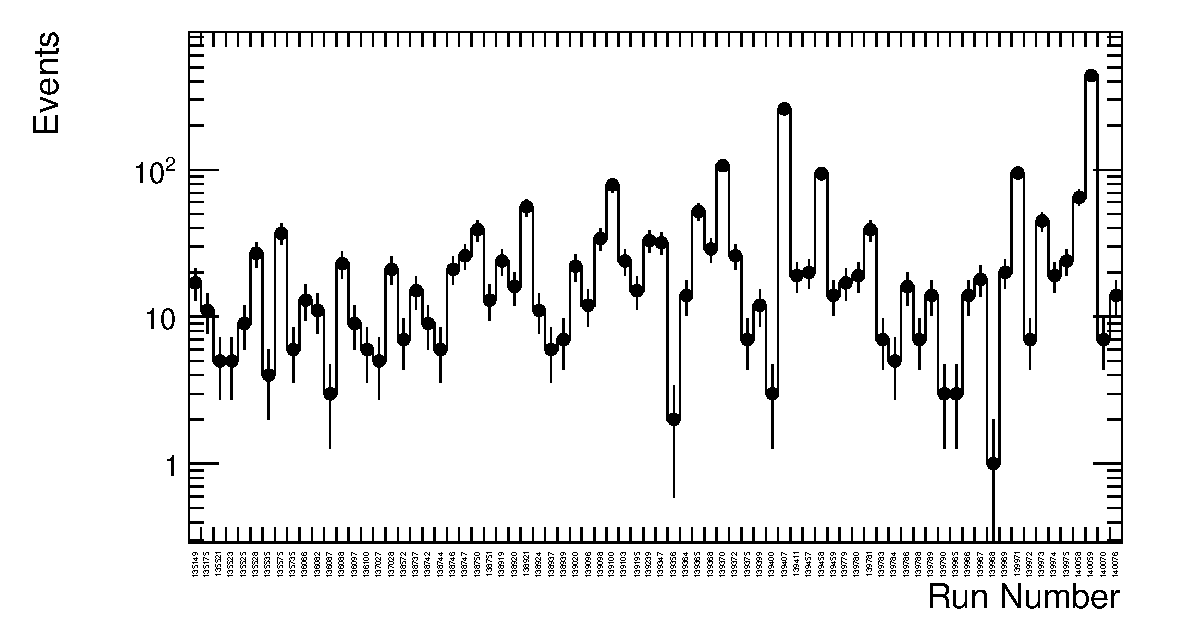
\includegraphics[width=0.9\textwidth]{Figures/Events.pdf}
\caption{Mean dijet mass vs run for runs with integrated luminosity greater than $1 nb^{-1}$ .}
    \label{MassVsRun}
  \end{center}
\end{figure}

\begin{figure}[!ht]
  \begin{center}
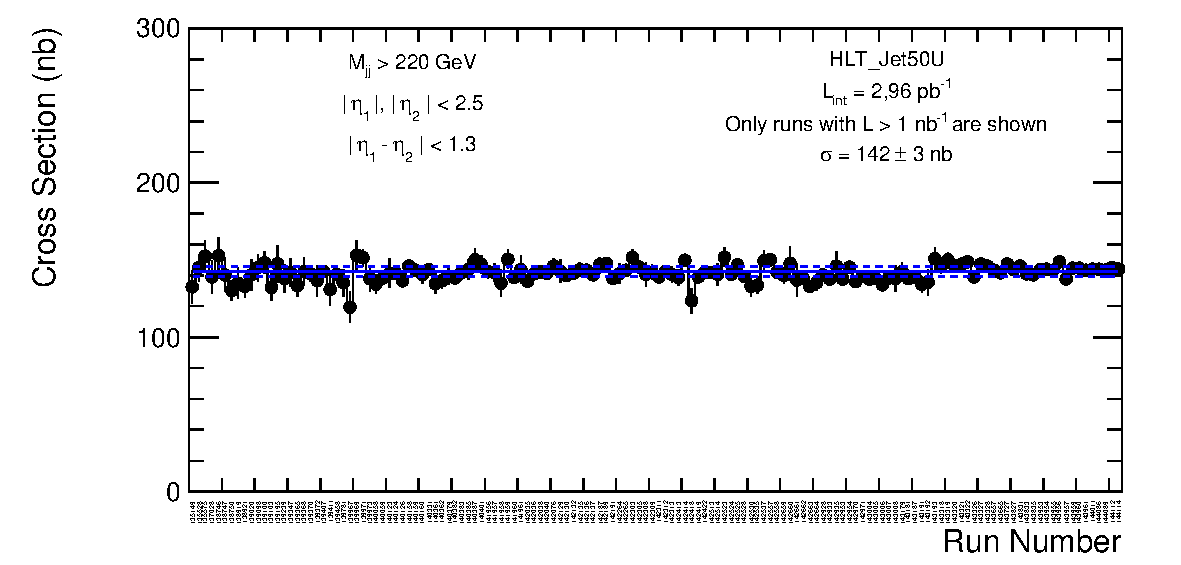
\includegraphics[width=0.90\textwidth]{Figures/XsecVsRunNo.pdf}
\caption{Number of dijet events passing the full selections, divided by the integrated luminosity of each run, vs. run.
Only runs with integrated luminosity greater than 1 $nb^{-1}$ passing the analysis selection are shown.}
    \label{XsecVsRun}
  \end{center}
\end{figure}

\begin{figure}[!ht]
  \begin{center}
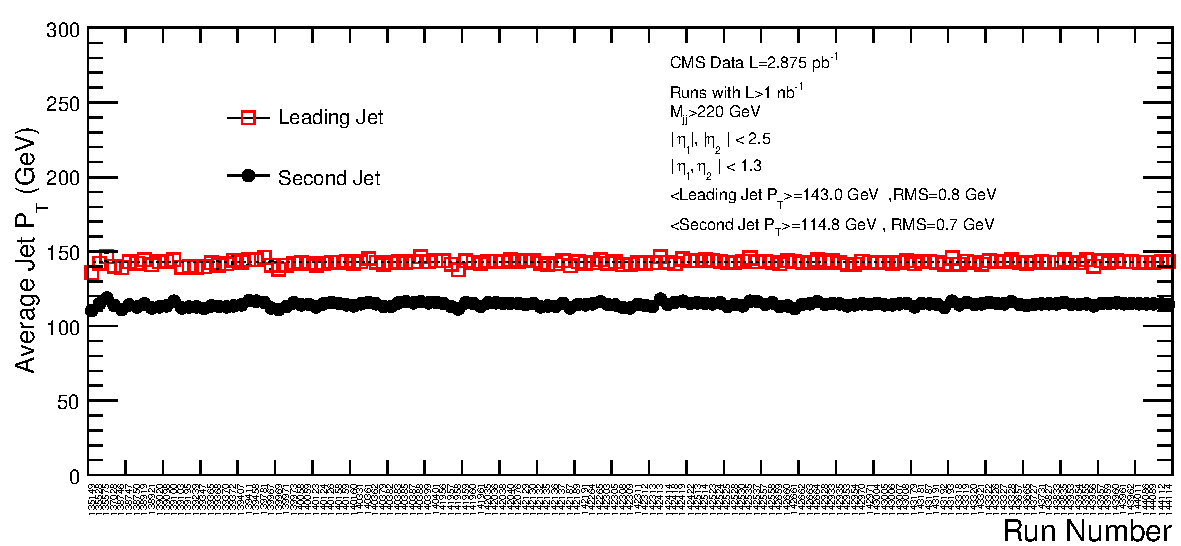
\includegraphics[width=0.49\textwidth]{Figures/PtVsRunNo.pdf}
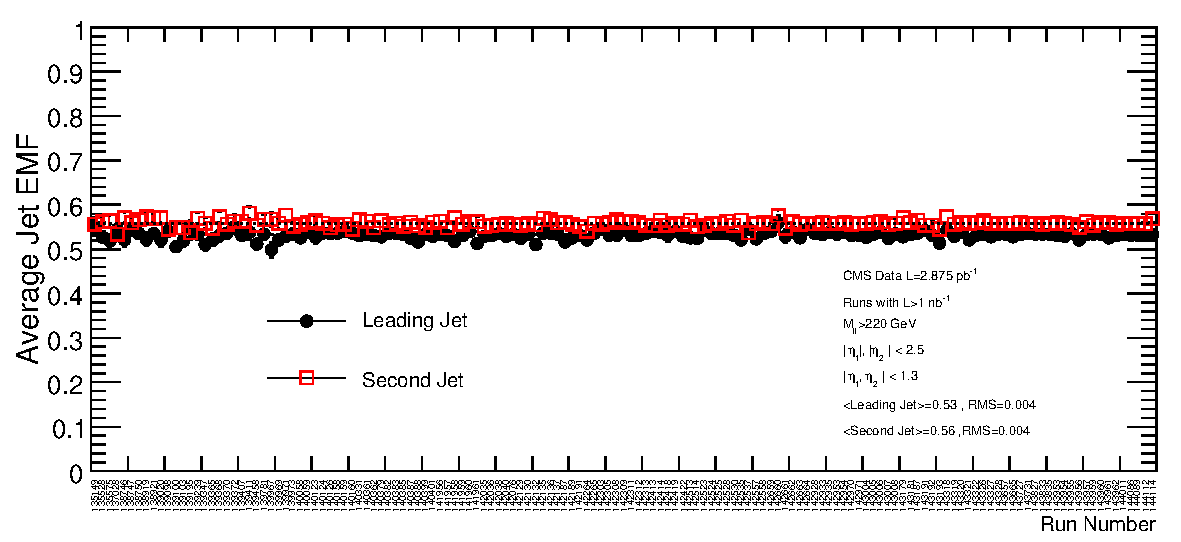
\includegraphics[width=0.49\textwidth]{Figures/EmfVsRunNo.pdf}
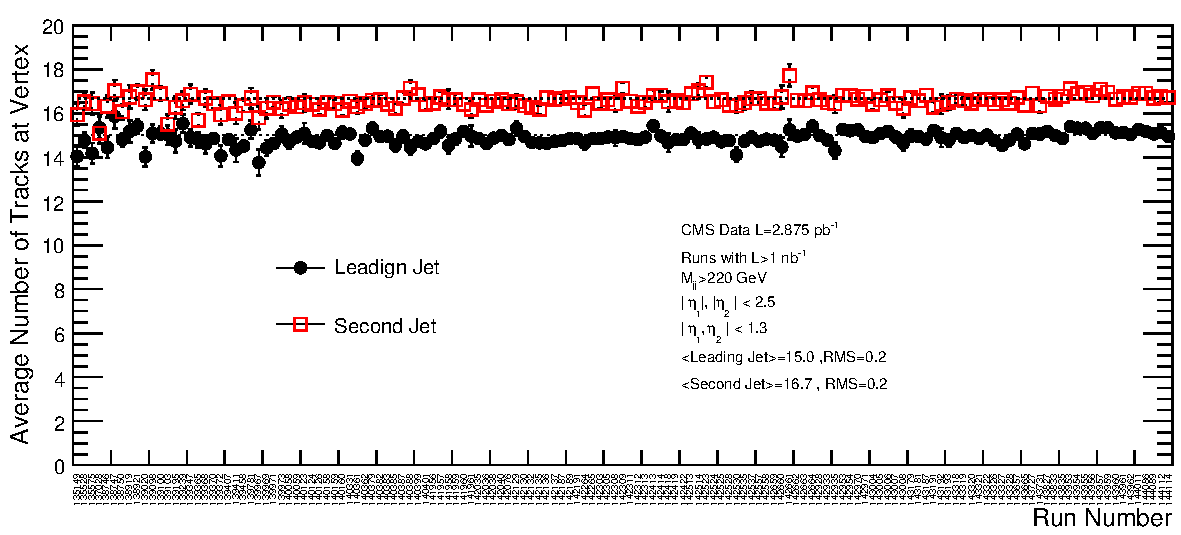
\includegraphics[width=0.49\textwidth]{Figures/NtrkVtxVsRunNo.pdf}
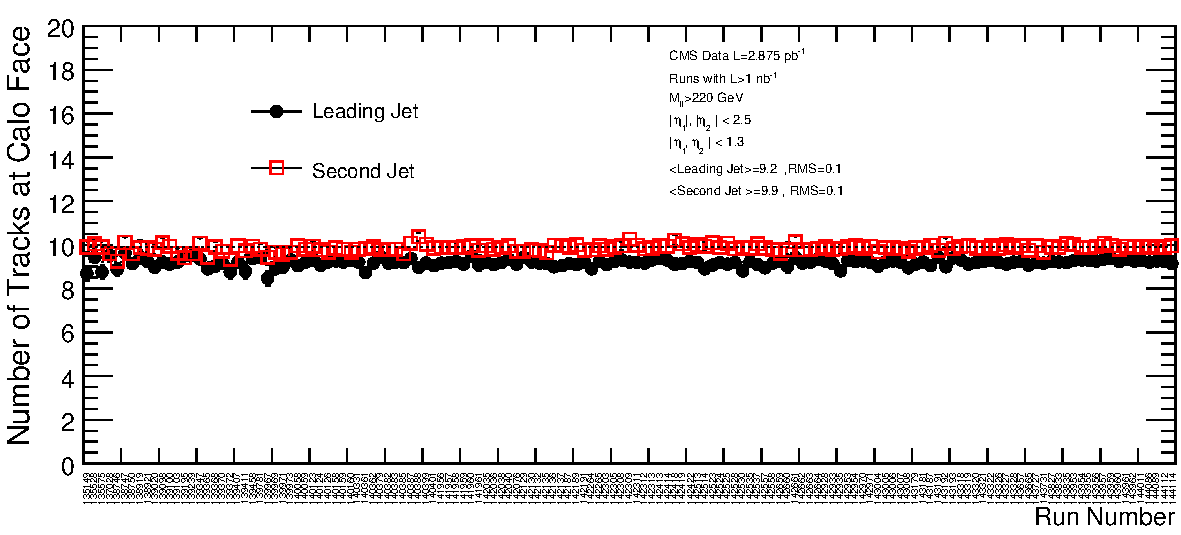
\includegraphics[width=0.49\textwidth]{Figures/NtrkCaloVsRunNo.pdf}
\caption{Mean value of jet properties for the leading jet (solid circles) and the second jet (open squares) vs. run: 
\pt (Top-Left), EMF (Top-Right), number of tracks associated with the jets at the vertex (Bottom-Left), number of tracks associated with the jets at the calorimater face (Bottom-Right). Only runs with integrated luminosity greater than $1 nb^{-1}$ are shown.}
    \label{JetPropertiesVsRun}
  \end{center}
\end{figure}

\clearpage
\subsubsection{Spectrum and QCD}
The measured dijet mass spectrum is shown in Fig~\ref{Spectrum}. The mass spectrum
is defined by 

\begin{equation}
\frac{d\sigma}{dm} = \frac{1}{\int Ldt} \frac{N_{i}}{\Delta m_i}
\label{eqXsec}
\end{equation}
where $m$ is the dijet mass, $N_i$ is the number of events in the $i$-th dijet mass bin, and $\Delta m_i$ is the width of the $i$-th 
dijet mass bin, and the integrated luminosity is $\int Ldt$.
This data is also tabulated in Appendix~\ref{appData}.  The bin width is approximately the dijet mass 
resolution, and gradually increases as a function of mass.
The data is compared to a QCD prediction from the PYTHIA MC and the full CMS simulation.
The normalization of the prediction is absolute, it has not been normalized to
the data in this plot.
Also shown in Fig~\ref{Spectrum} is the senstivity of the QCD + CMS simulation 
to a 10\% systematic uncertainty in the jet energy discussed in section~\ref{JESerror}.
The vertical error bars on the data are Poisson uncertainties, the horizontal
bars are the bin widths. Bins with zero events are indicated by a Poisson vertical error bar 
extending up to 1.8 events.
In Fig.~\ref{DataOverPythia} we show the ratio of 
the data to the PYTHIA prediction, which demonstrates at a fine scale the level of
agreement between data and PYTHIA. We can see that the 10\% uncertainty in the JES corresponds
to roughly a factor of 2 uncertainty in the observed cross section.
The PYTHIA QCD MC prediction is in good agreement with the data.   The highest mass dijet
event is at 2.05 TeV. 

%This can be seen from summation of the differential plot Fig~\ref{Spectrum} to 
%give the integral plot from the lower bin edge to infinity in Fig~\ref{Integral}. Conservatively,
%we expected 1 event above 1.4 TeV, and we observed 1 event above 1.4 TeV, and it happened to 
%occur at 2.13 TeV.  More aggressively, we expected 0.05 events above 2.1 TeV and we observed 
%1 event, which has a Poisson probability of 5\% which is still only about a 2 $\sigma$ effect.



\begin{figure}[!ht]
  \begin{center}
   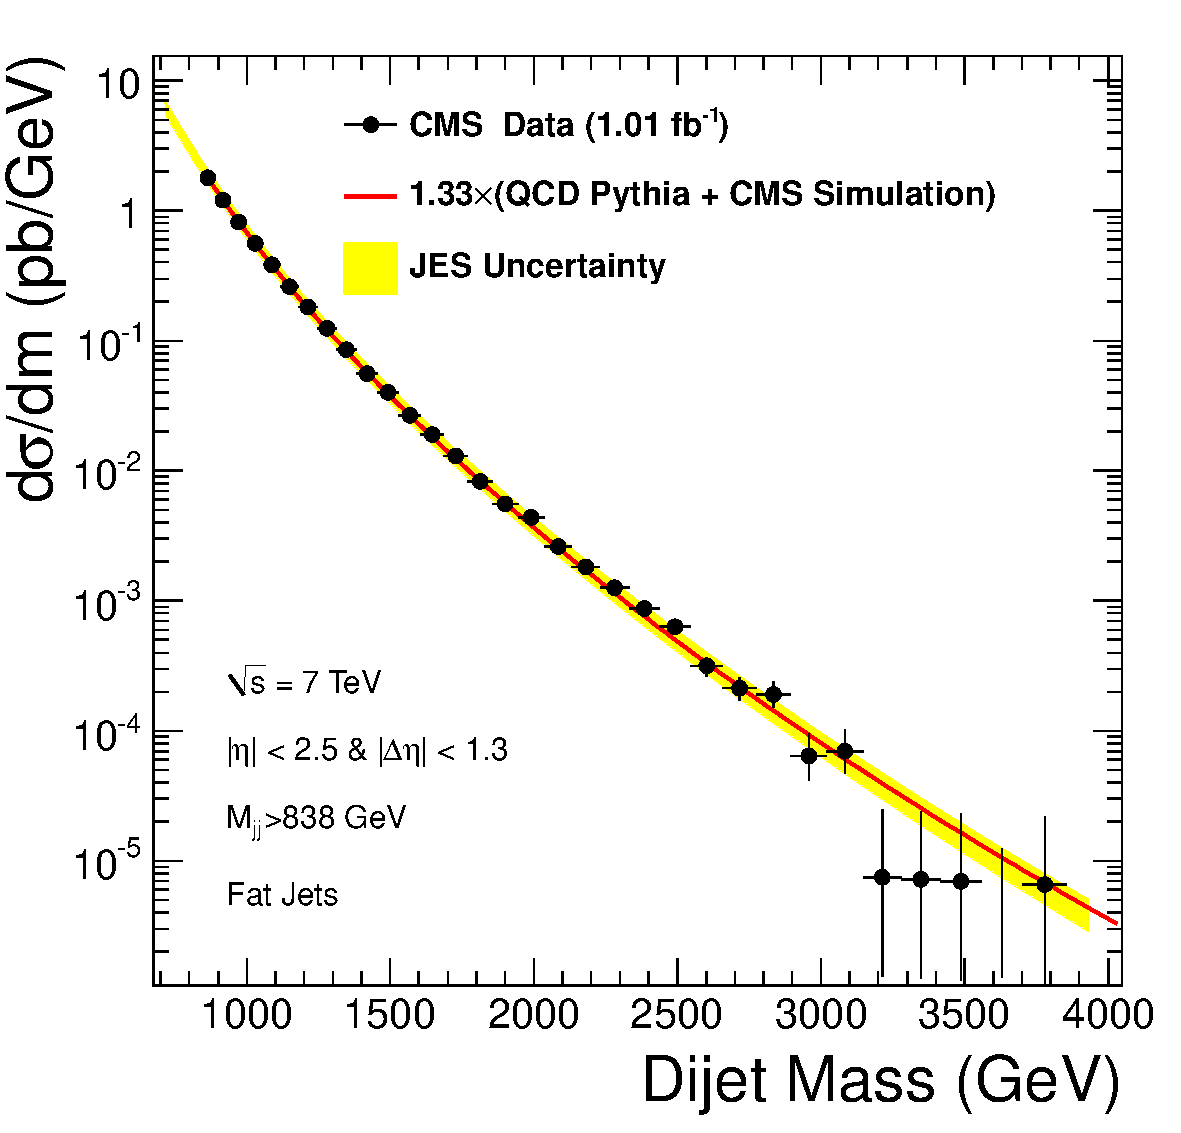
\includegraphics[width=\textwidth]{Figures/dijet_mass_Xsec.pdf}
    \caption{ The dijet mass spectrum data (points) is compared to a QCD MC prediction (histogram). Both the
    data and QCD prediction are absolutely normalized using the integrated luminosity.
    The band shows the sensitivity to a 10\% systematic uncertainty on the jet energy scale.}
    \label{Spectrum}
  \end{center}
\end{figure}

\begin{figure}[!ht]
  \begin{center}
   \includegraphics[width=\textwidth]{Figures/data_over_pythia.pdf}
    \caption{ Ratio of the dijet mass spectrum divided by the QCD Pythia prediction. Both the
    data and QCD prediction are absolutely normalized using the integrated luminosity.
    The band shows the sensitivity to a 10\% systematic uncertainty on the jet energy scale.}
    \label{DataOverPythia}
  \end{center}
\end{figure}

%\begin{figure}[!ht]
%  \begin{center}
%   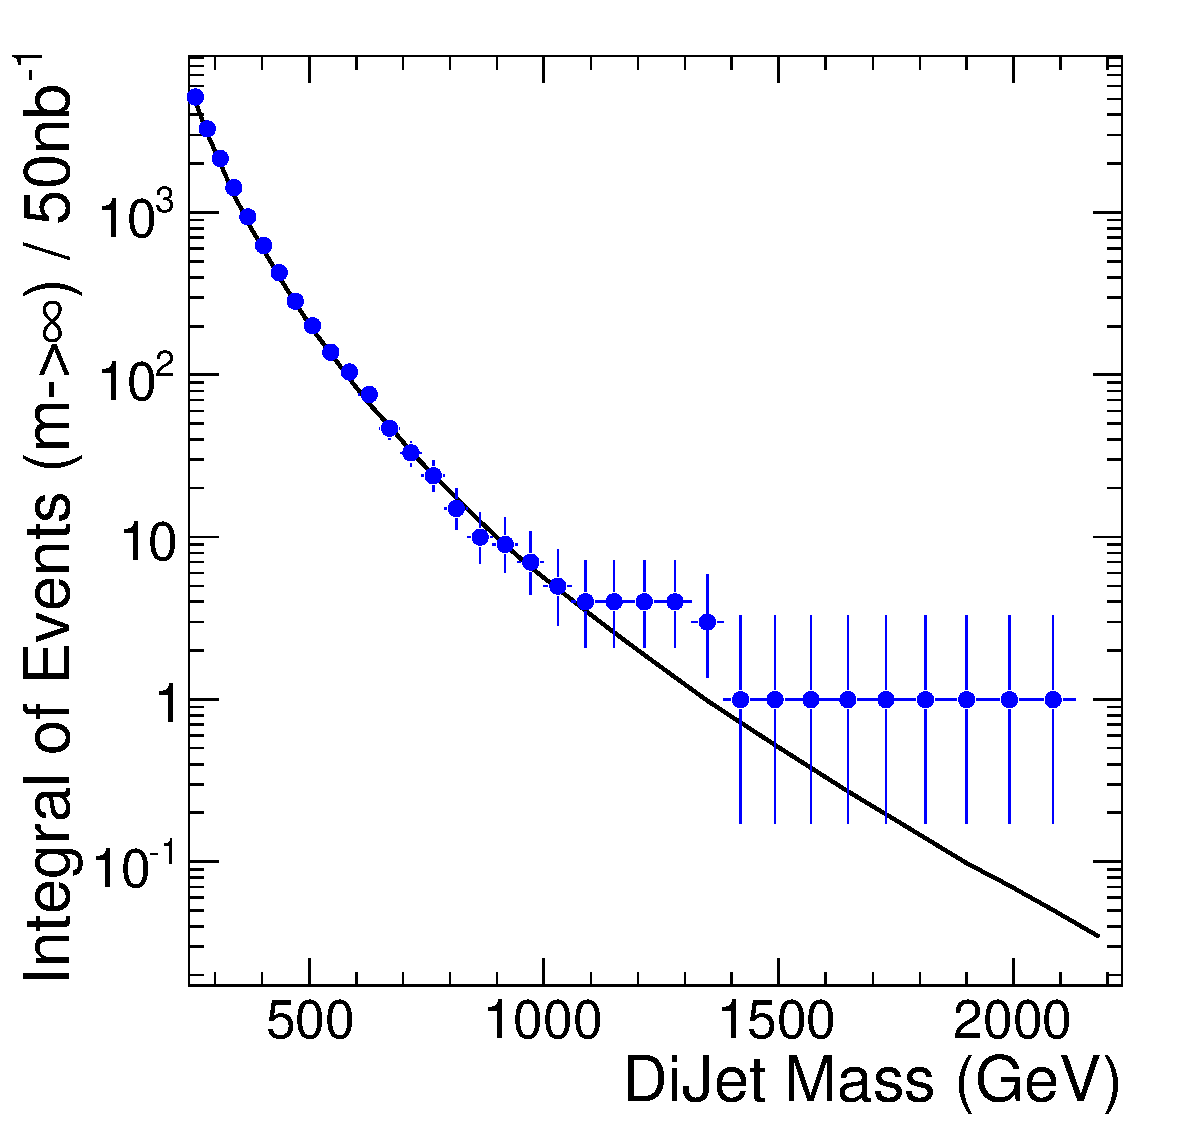
\includegraphics[width=\textwidth]{Figures/EventIntegral.pdf}
%    \caption{ The integrated event rate above a dijet mass threshold for the data (points) and 
%    the PYTHIA QCD prediction (curve).  The thresholds correspond to the lower edge of the mass bins
%    used in Fig.~\ref{Spectrum} and \ref{DataOverPythia}. The statistical errors on the points are 
%    highly correlated, because each point contains all the other points with higher dijet mass threshold.}
%    \label{Integral}
%  \end{center}
%\end{figure}

\clearpage

\subsection{Systematic Uncertainty on Jet Energy Scale}
\label{JESerror}
The jet energy systematic uncertainty band shown in Fig.~\ref{Spectrum} comes
from the JetMET guideline uncertainty of 10\% in the jet energy scale.
It is, by far, the dominant uncertainty in the measurement of the dijet
mass spectrum, and is also one of the largest uncertainties in the new particle
search.  The jet energy uncertainty at CMS is currently being explored with
in situ measurments which will ultimately provide a measure 
of the actual uncertainty~\cite{PAS_JME_07-002}.


As of today we can already see 
from measurements of photon plus jet balance~\cite{PAS_JME_10-003, CMS_AN_2010/141}
that the jet energy scale in the MC may very well be better than the 10\% currently being assigned. 
The jet response measured with photon + jet balance in the data, 
is in good agreement with the same response measured with the MC~\cite{PAS_JME_10-003} and constrain 
any difference to be well within the quoted 10\%. Due to the low statistics and
poorly understood calibration systematics and this early stage of the calibration analysis, JetMET
is not quoting an error yet based on this data, but JetMET is confident that the data do
indicate that 10\% is safe. 


At an even more fundamental level, we already see from
measurements of single particle response~\cite{PAS_JME_10-008, CMS_AN_2010/179}, that
the barrel calorimeter is responding as expected to input charged particles to better than 3\%.
Since a jet is made up of particles the uncertainty in the jet response can be 
constrained by the uncertainty in the constituent particle response.  The most uncertain
component is the charged pion response, as neutral pions are the other dominant contributor and they have well
understood response in the barrel ECAL.  The response of the ECAL plus HCAL to isolated 
charged particles measured in the barrel shows excellent agreement between
data and MC. Further, the MC simulation was tuned on test beam measurements of charged pions over
a wide range of momentum, and the tuning was quoted to be good to within 3\%.  Given these facts,
it is highly unlikely that the jet energy scale could be off by more than 10\% 
in the barrel.

We have also checked the energy scale of CaloJets against the energy scale
of particle flow jets in Figure~\ref{PFresp}.  Starting with the 
two leading PF jets in the event with $|\eta|<1.3$, we find the matching CaloJets that
are closest in $\Delta R$, plot the ratio of the corrected CaloJet to 
corrected PF jet $p_T$, and find the mean. The corrected CaloJet $p_T$ 
is in good agreement with the corrected PF jet $[_T$, well within 2\% at all 
$p_T$, demonstrating good agreement
between the jet energy scale defined by calorimetry alone and the jet energy
scale defined by tracking and calorimetry combined.
\begin{figure}[!ht]
  \begin{center}
   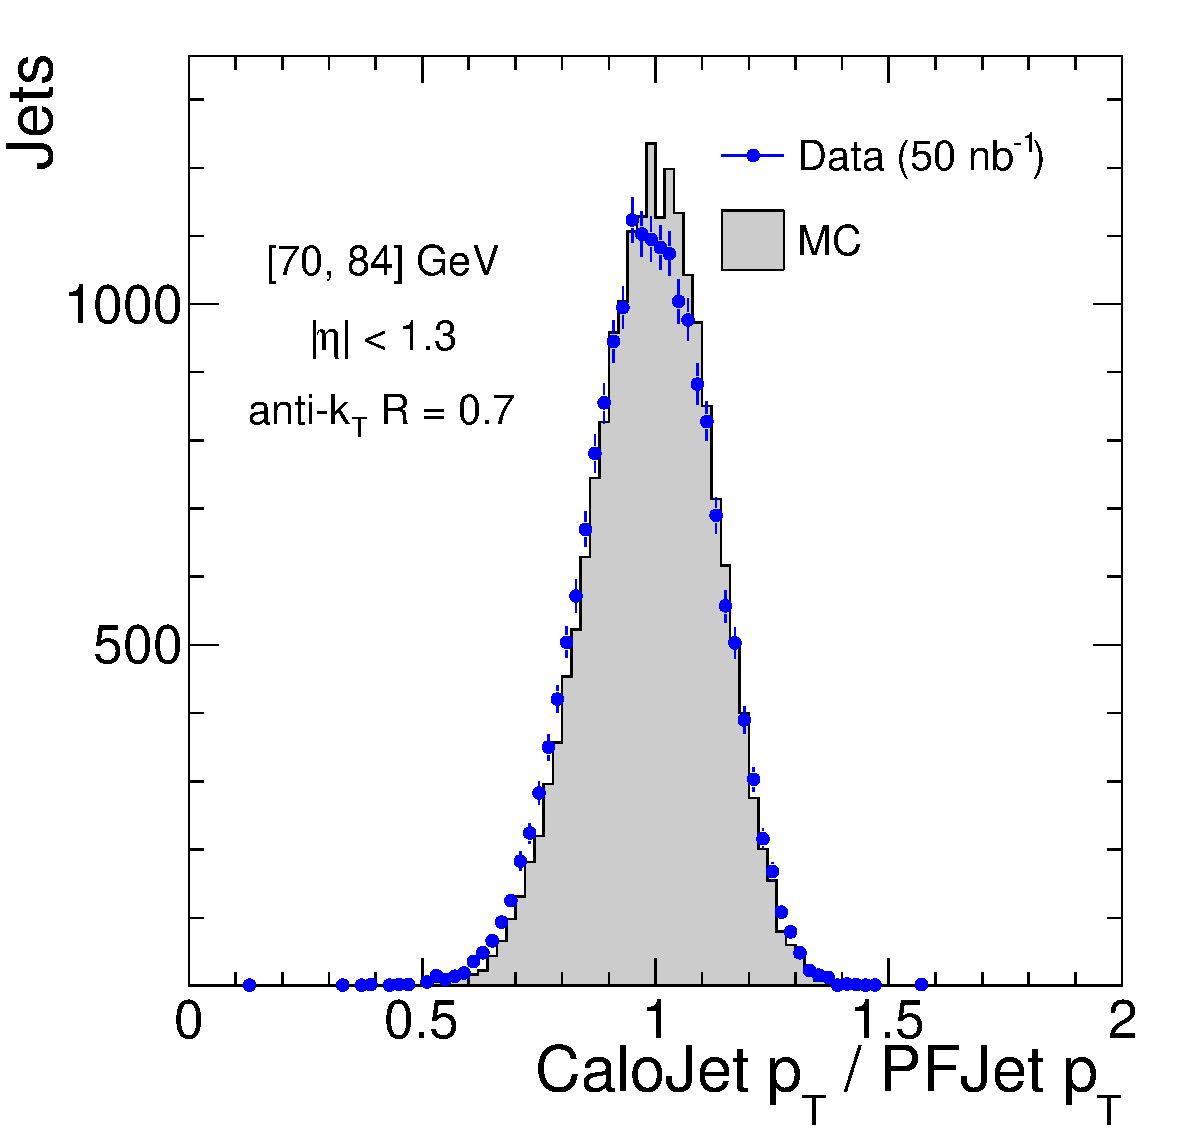
\includegraphics[width=0.32\textwidth]{Figures/caloRsp_Pt70to84.pdf}
   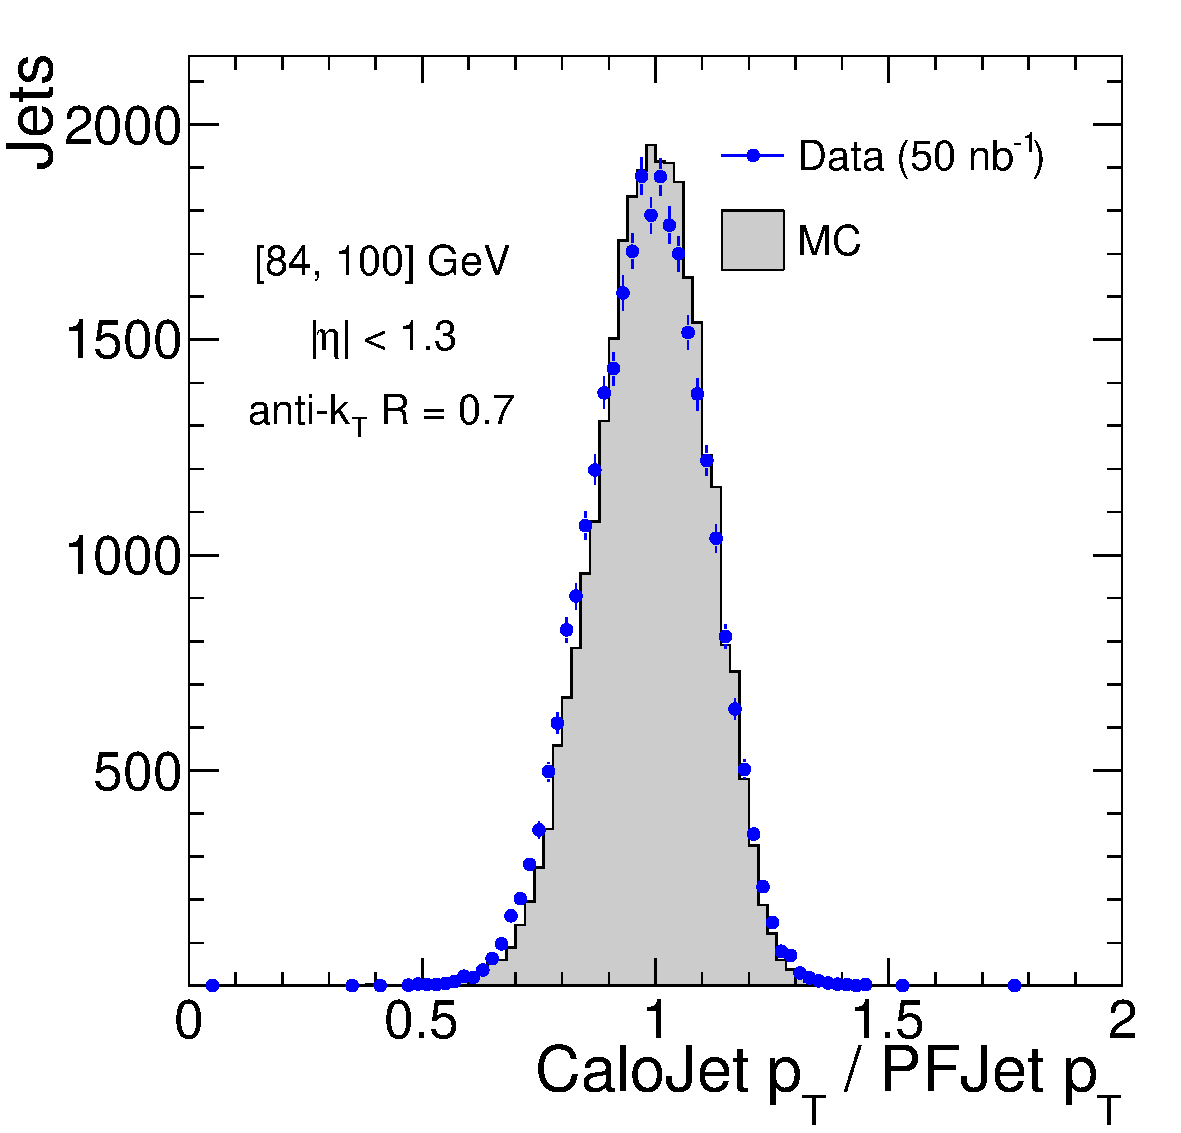
\includegraphics[width=0.32\textwidth]{Figures/caloRsp_Pt84to100.pdf}
   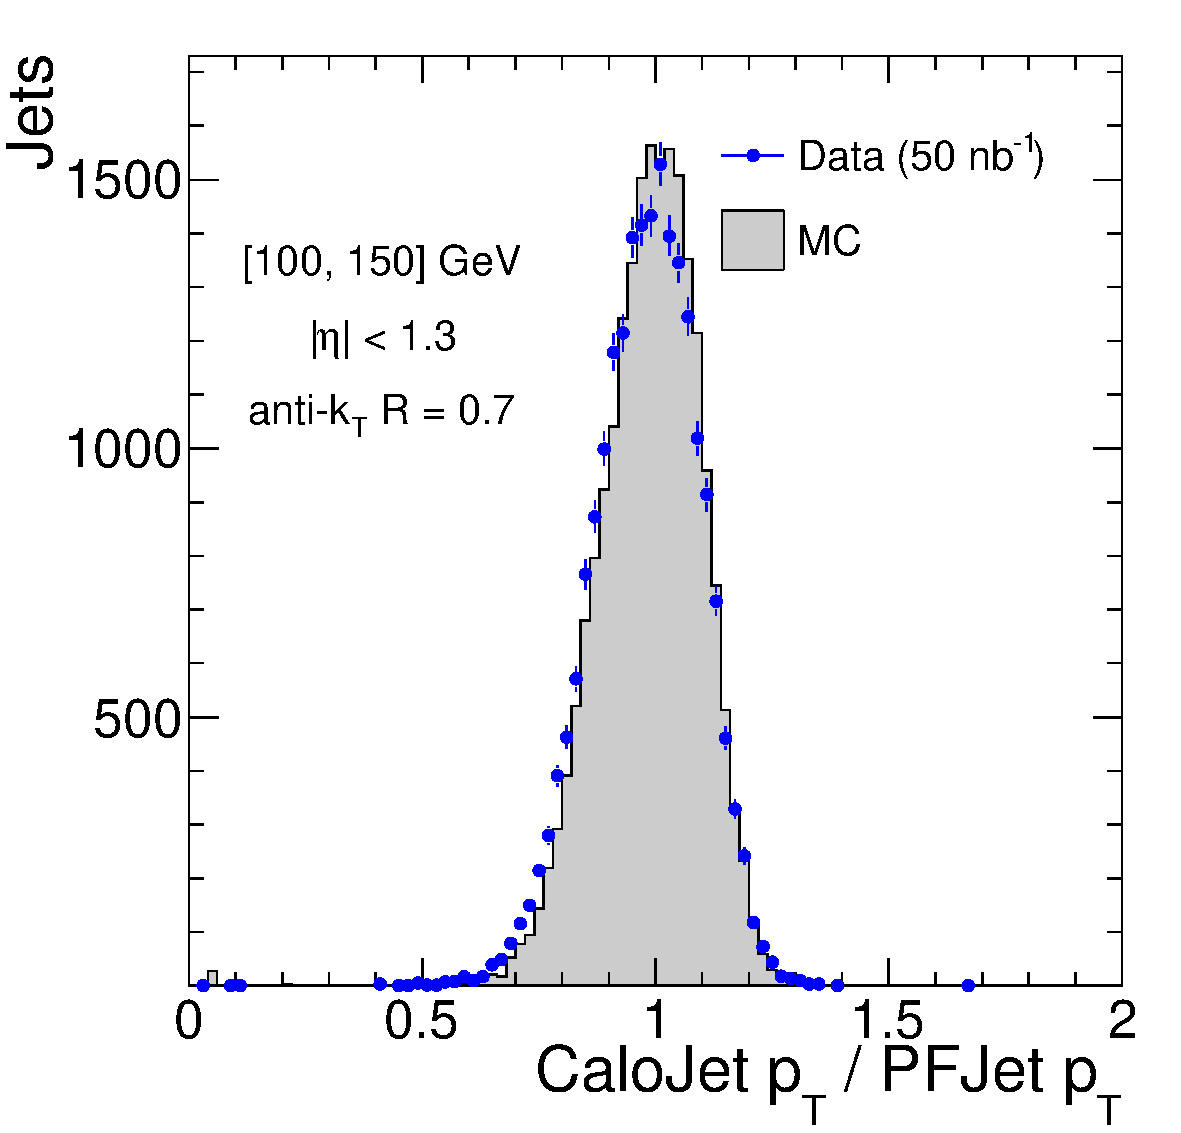
\includegraphics[width=0.32\textwidth]{Figures/caloRsp_Pt100to150.pdf}
   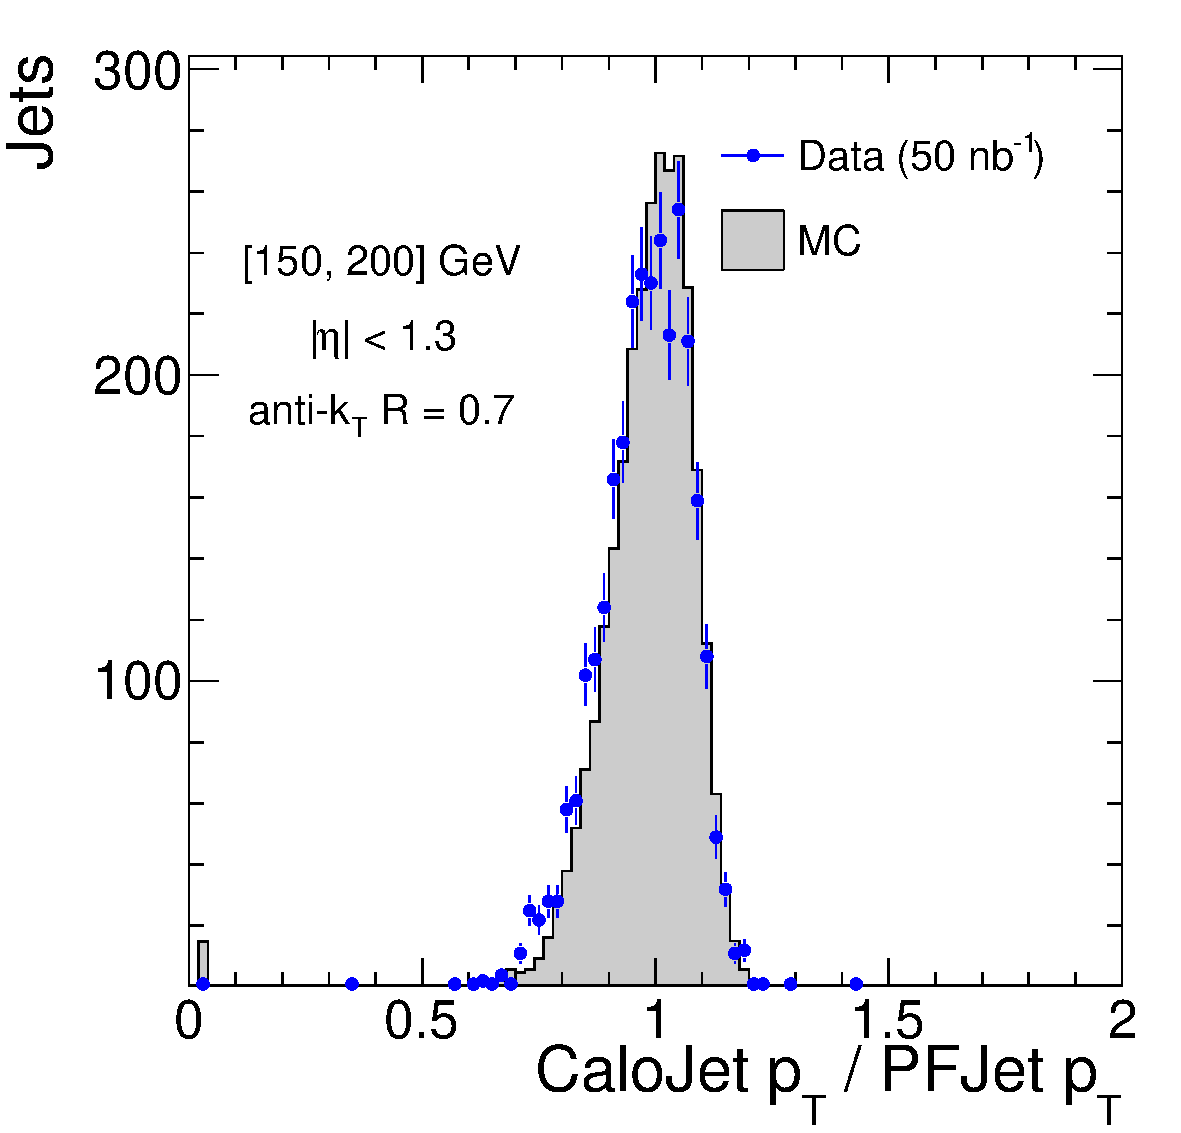
\includegraphics[width=0.32\textwidth]{Figures/caloRsp_Pt150to200.pdf}
   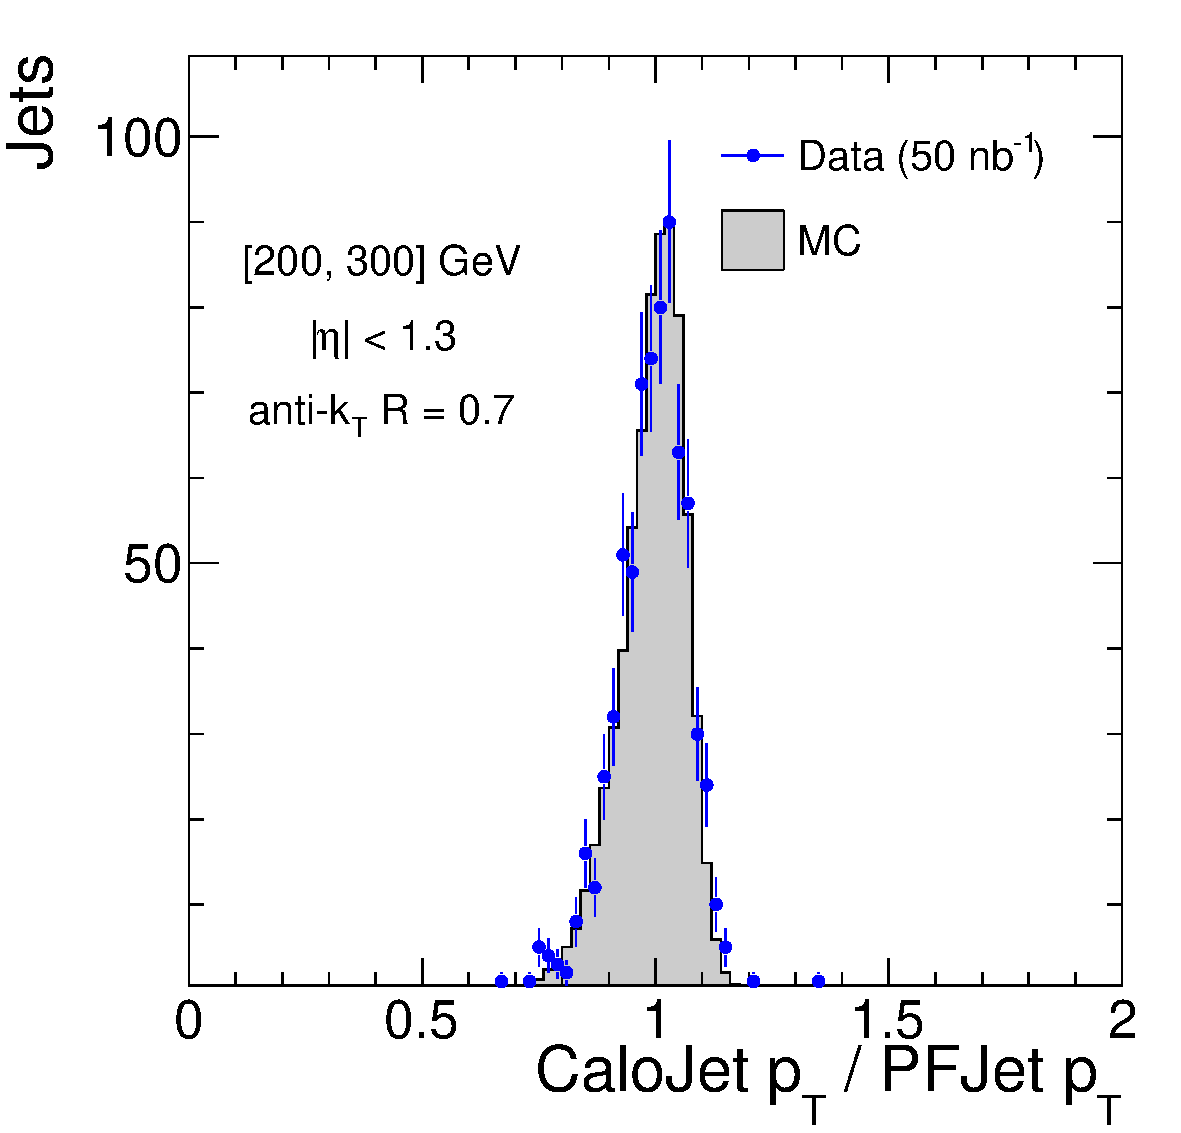
\includegraphics[width=0.32\textwidth]{Figures/caloRsp_Pt200to300.pdf}
   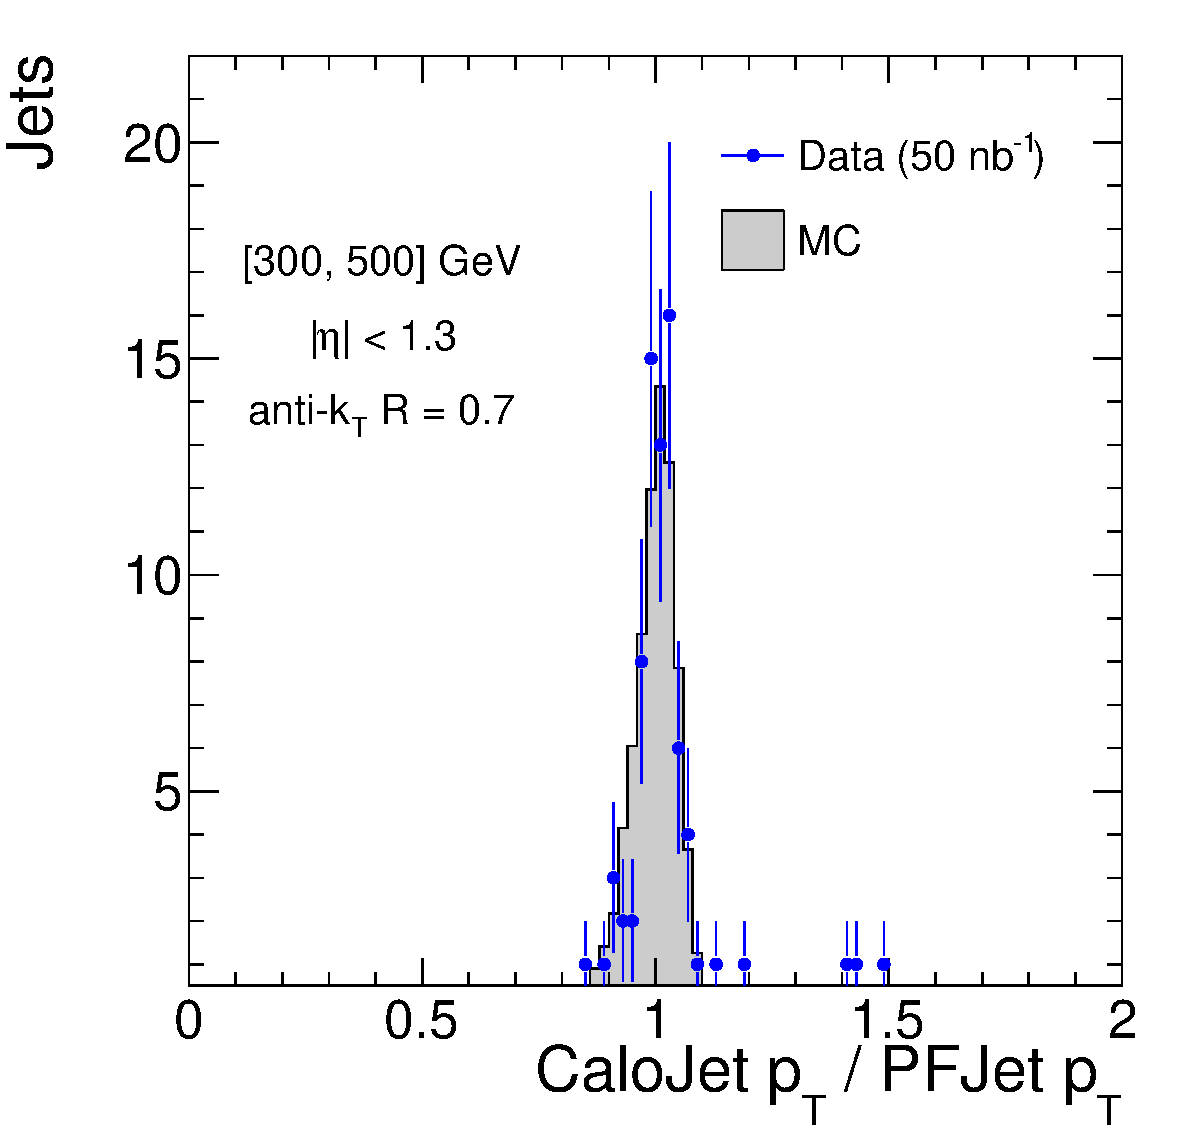
\includegraphics[width=0.32\textwidth]{Figures/caloRsp_Pt300to500.pdf}
   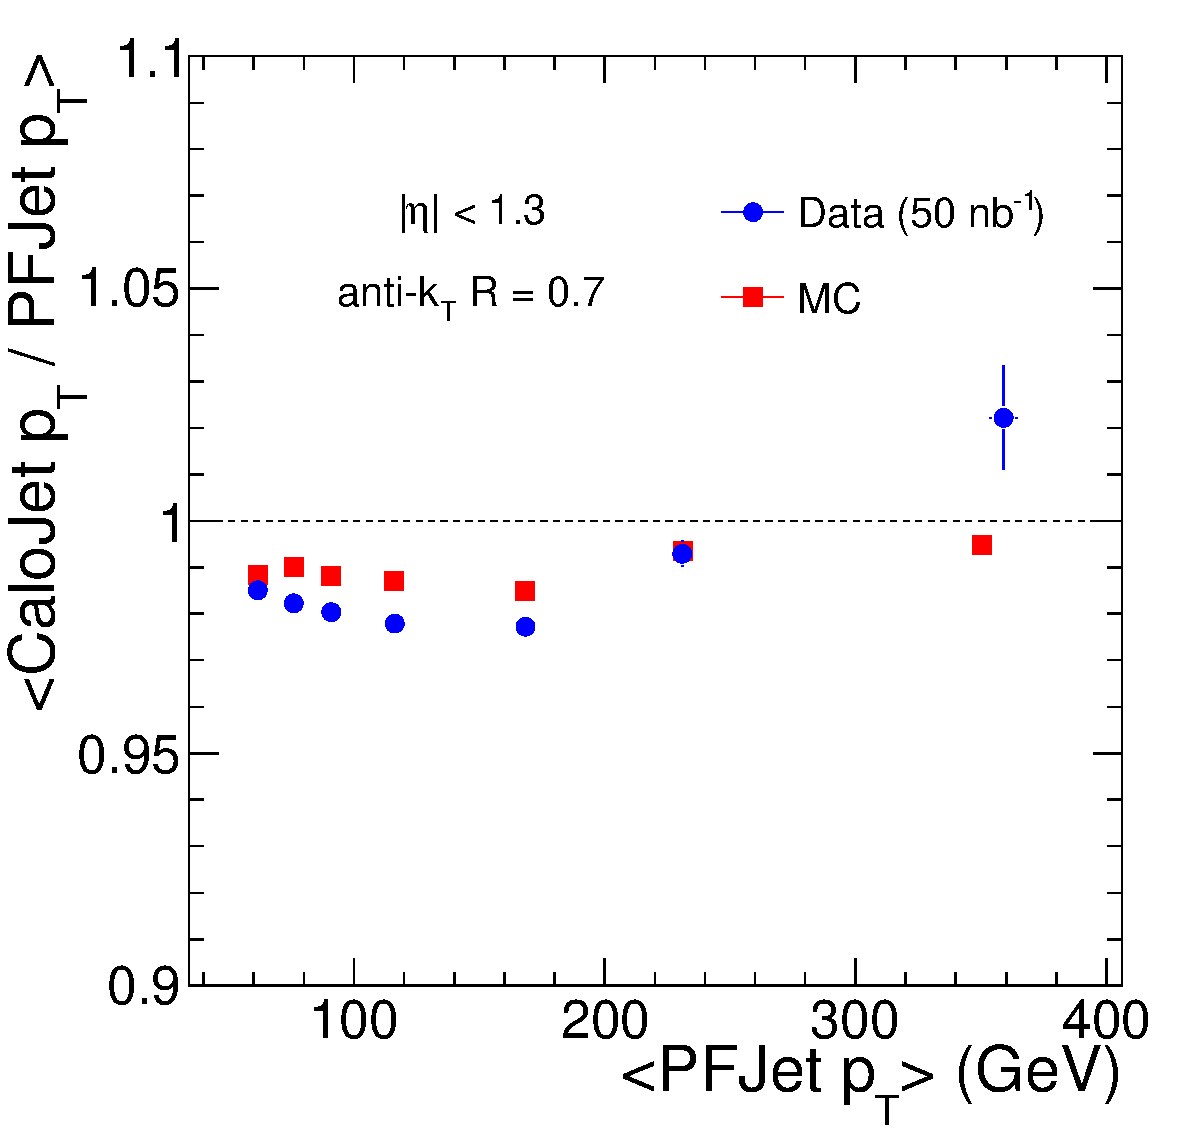
\includegraphics[width=0.8\textwidth]{Figures/PFvsCalo.pdf}   
    \caption{Distributions of Corrected CaloJet $p_T$ / Corrected PFJet $p_T$ 
    for leading jets which have $|\eta|<1.3$ 
    for six intervals of Corrected PF jet $p_T$ (top six plots) and the mean value of 
    this relative response as a function of the mean Corrected PF jet $p_T$ 
    (bottom plot).}
    \label{PFresp}
  \end{center}
\end{figure}

In situ data indicate that the 10\% guideline provided by JetMET on the jet energy scale uncertainty
is a conservative (safe) estimate.  

\subsection{Highest Mass Dijet Events}

Event displays of the ten highest mass dijet events are shown in 
Appendix~\ref{appEvents}.  They all look like good events, with
collimated calorimeter energy deposits and associated tracks.  Table~\ref{table_highmass2} in the 
Appendix lists the basic properties of 
the calorimeter reconstrution for these events.  
The highest
dijet mass observed is at 1.92 TeV as already mentioned. 

%In Appendix~\ref{appEvents} in table~\ref{table_highmass3} we list the 
%$p_T$ and dijet mass for these events from particle flow reconstruction
%of the jets (PFjets), which employs tracking in addition to the calorimeter.
%The $p_T$ and dijet mass values are very similar.  Here the PFjets have been
%matched to the corresponding leading CaloJets and are shown in that order
%in table~\ref{table_highmass3}.

%In Fig.~\ref{PF}, we
%show the difference in corrected jet $p_T$ between the leading 
%CaloJets and particle flow jets.
%The mean difference is $\Delta p_T= -0.5$ GeV out of 
%about 300 GeV.  The RMS of the difference between CaloJets and
%PFJets is 15 GeV.  This is in good agreement with the expected RMS from the 
%MC of 18 GeV: this expected RMS takes into account significant correlations 
%between the two reconstruction techniques~\cite{refMikko}. The mean 
%difference of the dijet mass between the two techniques is $2\pm 10$ GeV, 
%and the RMS of the difference in dijet mass is 33 GeV, which makes sense compared
%to $p_T$, but we do not have 
%available an estimate of this RMS from MC that takes into account correlations.
%The good agreement
%between calorimeter and particle flow jet reconstruction techniques for 
%the 10 highest mass dijet events indicates that jet reconstruction with 
%tracking is confiriming our 
%calorimeter based reconstruction technique.


%\begin{figure}[!ht]
%  \begin{center}
%   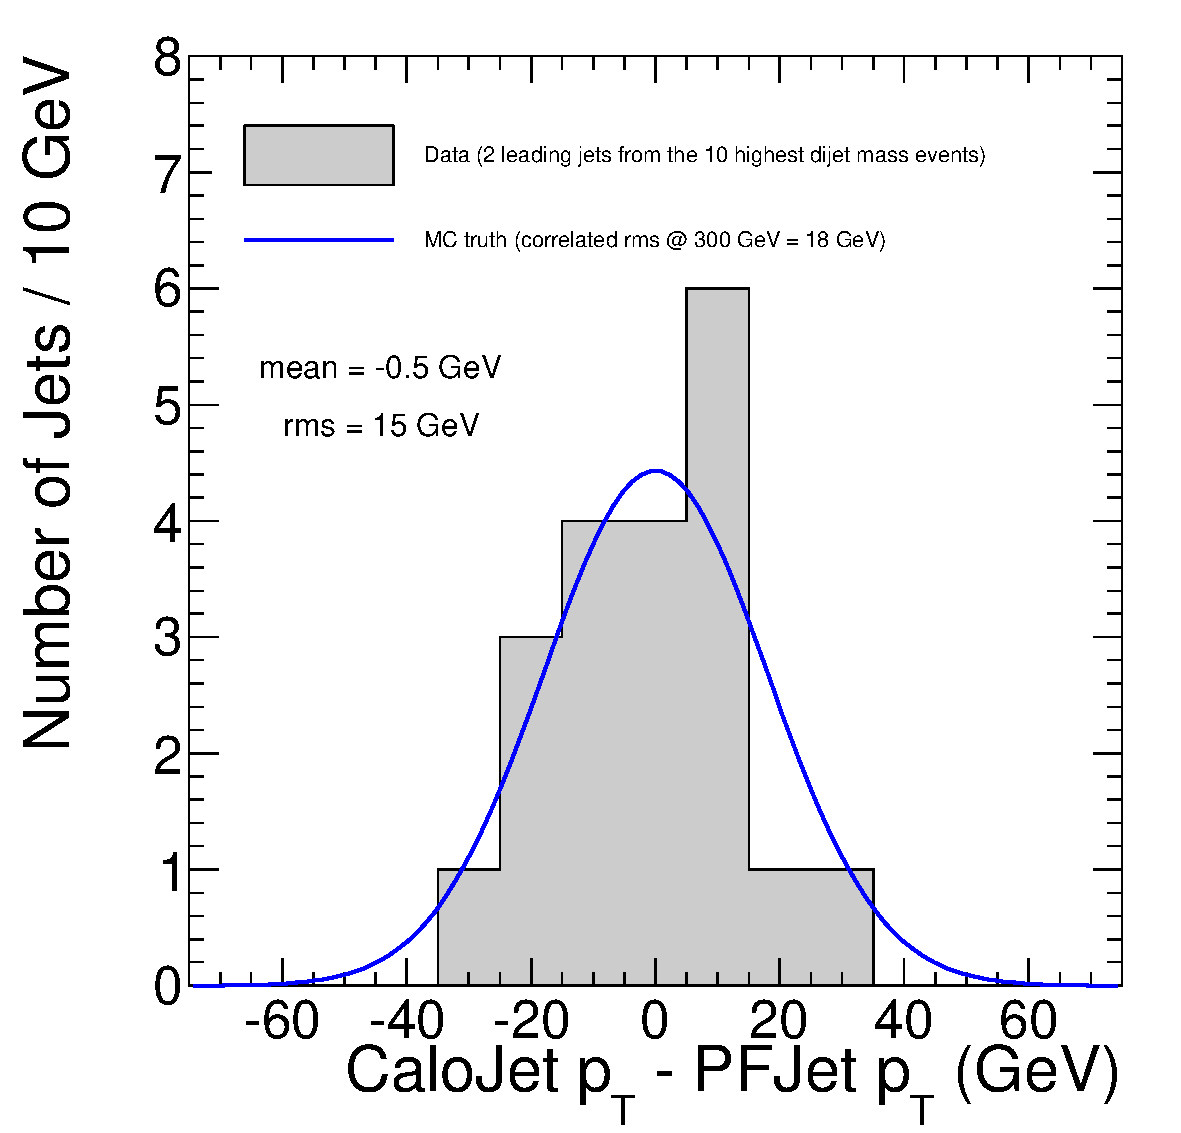
\includegraphics[width=0.7\textwidth]{Figures/CaloPFCorrelation.pdf}
%    \caption{The difference in corrected jet $p_T$ between the leading CaloJets
%    and the leading matched particle flow jets (histogram) for the 10 highest dijet
%    mass events is compared with an estimate of the expected difference from MC (curve)
%    taking into account correlations. }
%    \label{PF}
%  \end{center}
%\end{figure}
\clearpage

\subsection{Dijet Mass Spectrum and Fit}


\begin{figure}[!ht]
  \begin{center}
   \includegraphics[width=\textwidth]{Figures/DijetMass_withFit.pdf}
    \caption{The dijet mass distribution (points) compared to a smooth background fit (solid
curve). }
    \label{Fit}
  \end{center}
\end{figure}


Fig.~\ref{Fit} shows the dijet mass spectrum from Fig.~\ref{Spectrum} compared to
a fit. Here we model the background to a dijet resonance coming from standard model dijet production
using a simple parameterization. Our first test for whether there is a bump or other local
effect in the data is to simply see if we can get a good fit to a smooth parameterization.
Fig.~\ref{Fit} also shows the parameterization fitted to the data. We get a $\chi^2$ of 32.3 
for 31 degrees of freedom for the fit.  The parameterization chosen is~\cite{Aaltonen:2008dn,ATLAS_Search} 


\begin{equation}
\frac{{\rm d}\sigma}{{\rm d}m} = 
\frac{P_{0} (1 - m/\sqrt{s})^{P_{1}}}{(m/\sqrt{s})^{P_{2} + P_{3} ln
(m/\sqrt{s})}}
\label{eqParam}
\end{equation}

Fig~\ref{FracDiff} shows the fractional differences between data and the fit function, (data-fit)/fit, which show no significant evidence 
of a peaks above the background fit. The most significant upward fluctuation observed is studied in section~\ref{significance}. 
In the fractional difference plot the error bars are in units of the fit in the bin.
Fig.~\ref{FracDiff} show the pulls, defined as \textit {(Data-Fit)/Error}, which are consistent with statistical fluctuations and 
are oscillating around zero. In the pulls plot the error bars are always exactly 1, because they are in units of the error in the bin.

\begin{figure}[!ht]
  \begin{center}
        \includegraphics[width=0.9\textwidth]{Figures/Fractional_Diff.pdf}
    \includegraphics[width=0.9\textwidth]{Figures/Pulls.pdf}
    \caption{ \textit{Top})
The fractional difference between the dijet mass distribution (points) and a smooth
background fit as a function of dijet mass. \textit{Bottom}) The pulls distribution (Data-Fit)/Error as a function of dijet mass.}
    \label{FracDiff}
  \end{center}
\end{figure}
\clearpage
%%%%%%%%%%%%%%%
\subsubsection{Fit to Dijet Mass Spectrum with Various Parameterizations}
\label{sectionParam}

 
In Fig.~\ref{dijetmassFitParams} we show the dijet mass distribution,
$d\sigma/dm$, fit with three different parameterizations:  our default 4 parameter
fit and two alternate fits.
%%%%%%%%%%%%%%%%%%%%
\begin{figure}[!ht]
  \begin{center}
        \includegraphics[width=\textwidth]
                        {Figures/DijetMass_withFit_All.pdf}
    \caption{ 
The dijet mass data (points) is compared to fits (curves)
using our default fit function and three alternate fit functions.}
    \label{dijetmassFitParams}
  \end{center}
\end{figure}

\clearpage
The parameterizations are listed in equation~\ref{eqVariousParams}.

%%%%
\begin{eqnarray}
{\frac{d\sigma}{dm}} 
 &=& {\frac{P_{0} \cdot (1 - m/\sqrt{s})^{p_{1}}}{(m/\sqrt{s})^{p_{2} + p_{3} ln(m/\sqrt{s})}}} \, \, \, \mbox{(Default Fitwith 4-parameters)}. \cr
 & & \cr
 &=& {\frac{P_{0} \cdot {\Big(1-m/\sqrt{s}+P_3\cdot(m/\sqrt{s})^2\Big)^{P_1}}}{m^{P_{2}}}} \, \, \,\mbox{ (Alternate Fit A with 4-parameters)}. \cr
 & & \cr
 &=& {\frac{P_{0} \cdot {(1-m/\sqrt{s}\,)^{P_1}} }{m^{P_{2}}}}, \, \, \, \mbox{(Alternate Fit B with 3-parameters)} \cr
\label{eqVariousParams}
\end{eqnarray}
%%%%


The default four parameter function was used by CDF in run II~\cite{Aaltonen:2008dn} and is used 
by ATLAS~\cite{ATLAS_Search}. It gives a good fit with $\chi^2/DF=32.3/31$.
We have also explored two alternate parameterizations.  All parameterizations have a power law in them, because without
a power law we cannot get a good fit with only 3 or 4 parameters. 

Alternated fit B is a three parameter fit that was used by CDF in run IA~\cite{Abe:1995jz} and has the simplest QCD motivation,
althought all the parameterizations are motivated in a similar fashion.  It was used in much earlier versions of this CMS analysis
with significantly less luminosity.
It has a term in the numerator motivated by the parton distribution fall off
with fractional momentum, the same term as in the numerator of our default fit.
It includes a power law fall off with mass in the denominator, 
motivated by the QCD matrix element. The goodness of fit, $\chi^2/DF=39.3/32$, is significantly
worse than our default four parameter fit.

Alternate fit A is a 4-parameter function that was used by CDF 
in run IB~\cite{Abe:1997hm} and in the last version of this CMS analysis.
It similar to alternate fit B, except it has an additional term in the numerator to give flexibility beyond the
3-parameter fit. The goodness of fit, $\chi^2/DF=38.6/31$, is significantly worse than 
our default four parameter fit. Since this parameterization has the same number of 
parameters as our default fit, we use it to evaluate systematics on the background
functional form, and it should be conservative given the difference in $\chi^2$ between the
two fits.

Figure~\ref{dijetmassFits} shows the fractional 
differences between data and the fit function, (data-fit)/fit, 
and the pulls, (data-fit)/error, for all three fits.

%%
\begin{figure}[!ht]
  \begin{center}
        \includegraphics[width=\textwidth]{Figures/Fractional_Diff_All}
        \includegraphics[width=\textwidth]{Figures/Pulls_All}
    \caption{ Top) Fractional difference (points) between the dijet mass distribution 
data and four fits as a function of dijet mass.
Bottom) Pulls for the data (points) compared to four fits as a function of dijet mass.}
    \label{dijetmassFits}
  \end{center}
\end{figure}

%\begin{figure}[!ht]
%  \begin{center}
%        \includegraphics[width=0.8\textwidth]
%                        {Figures/dijet_mass_Fit_FracDiff_23params.pdf}
%    \caption{
%    Fractional difference between the dijet mass distribution 
%data points and the 2-parameter fit (left) and the 3 and 4 parameter fits (right).}
%    \label{dijetmassFractionalDiffFit23params}
%  \end{center}
%\end{figure}
%%%%%%%%%%%%%%%%%%%%

\clearpage



\section {Search for Dijet Resonance}

\subsection {The Signal: Dijet Resonance}


\begin{figure}[hbt]
  \begin{center}
      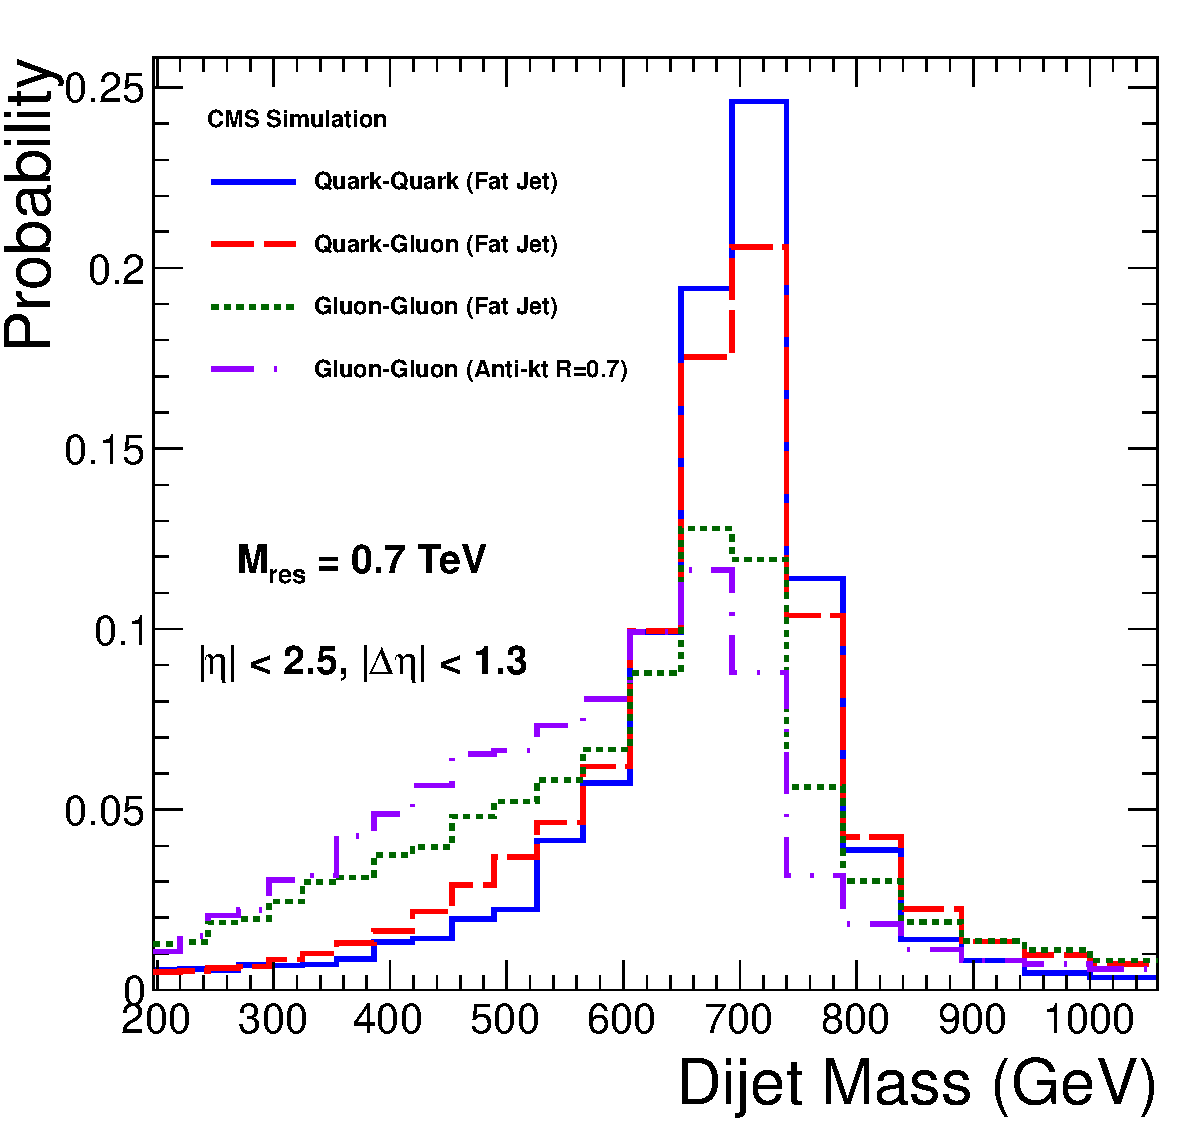
\includegraphics[width=0.45\textwidth]{Figures/shape_700GeV.pdf}
       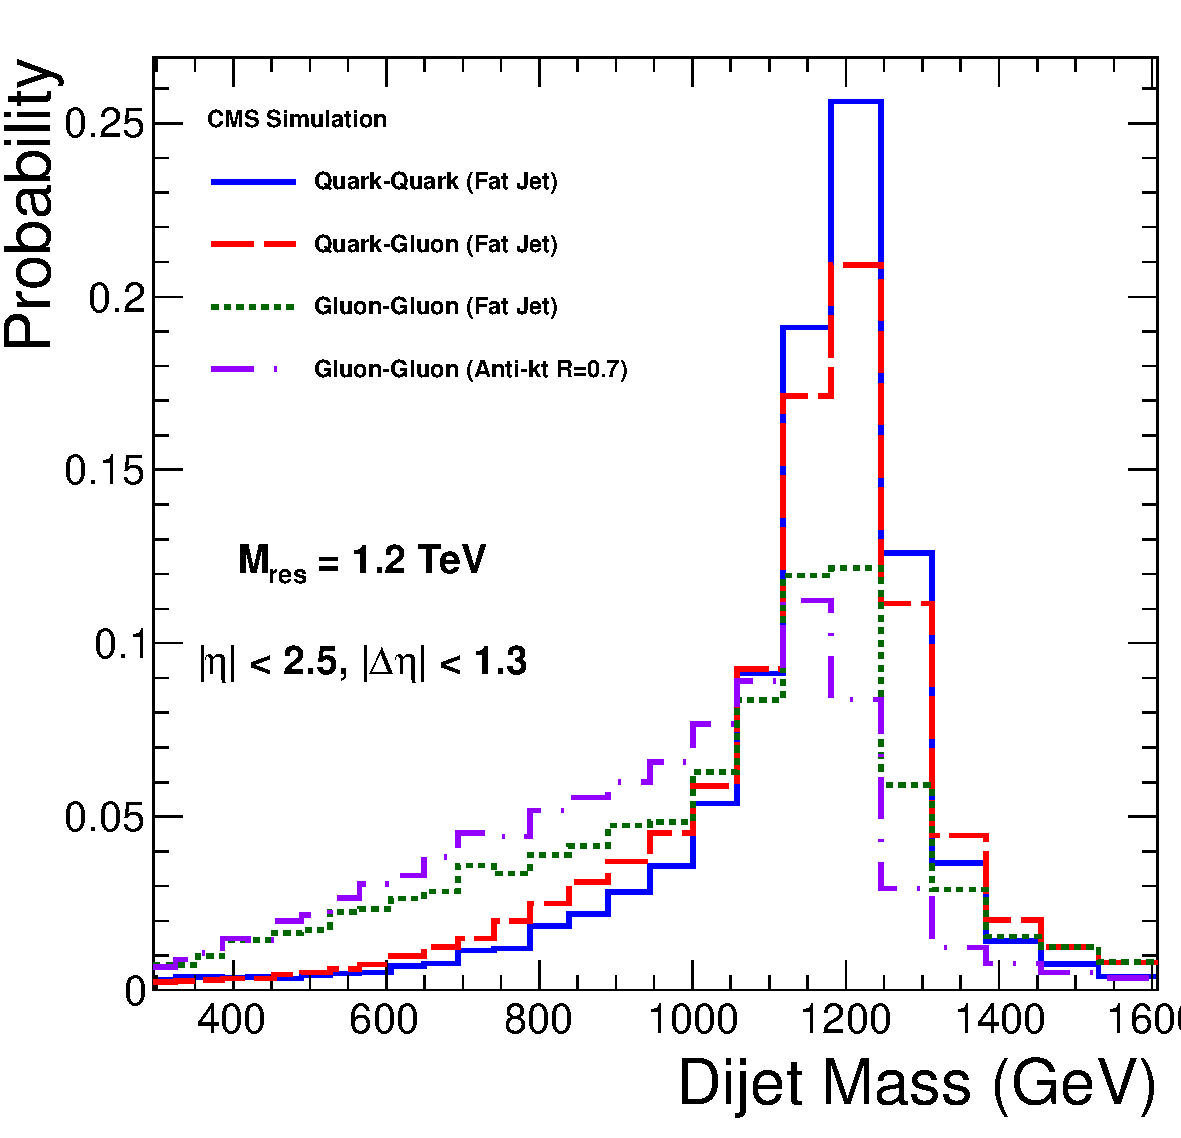
\includegraphics[width=0.45\textwidth]{Figures/shape_1200GeV.pdf}
       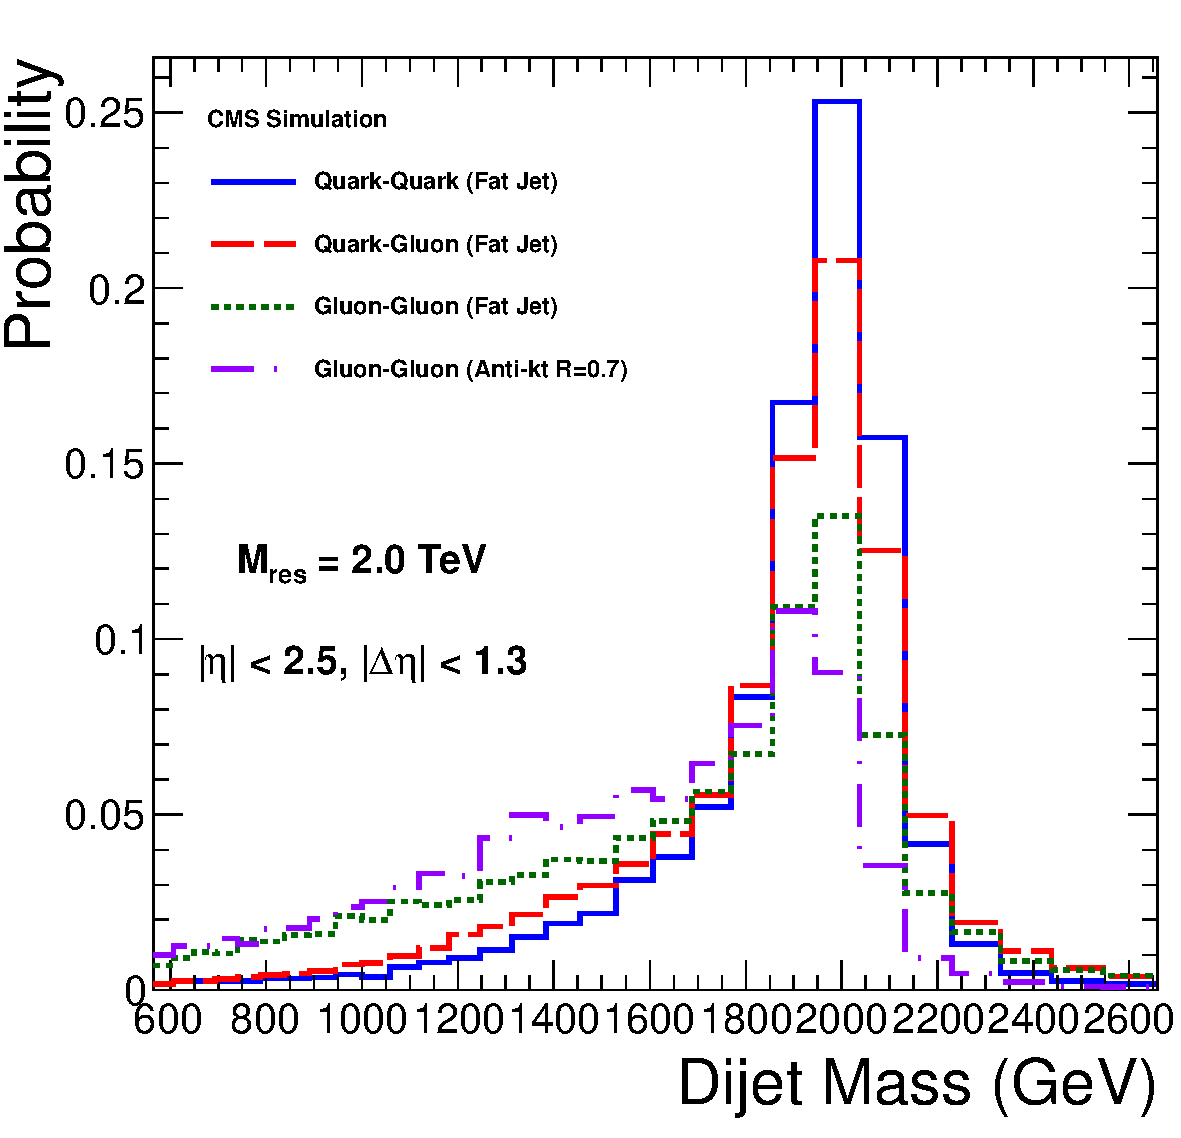
\includegraphics[width=0.45\textwidth]{Figures/shape_2000GeV.pdf}
        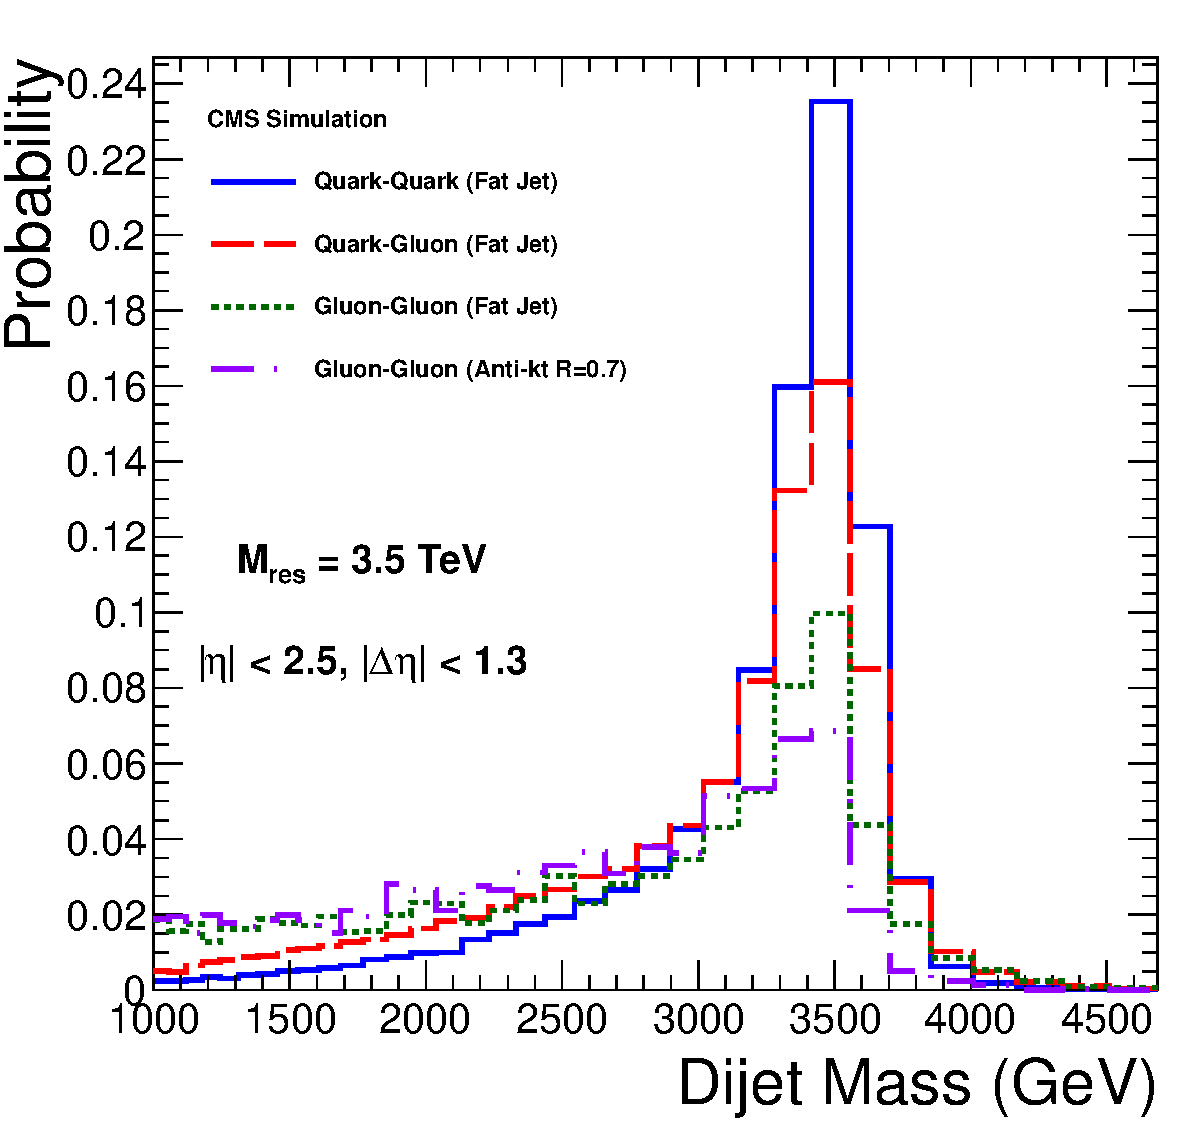
\includegraphics[width=0.45\textwidth]{Figures/shape_3500GeV.pdf}
    \caption{Dijet mass distribution for $q\bar{q}$ $(qq)$, $qg$ and $gg$ resonances at 
    $0.7$, $1.2$, $2$ and $3.5$ TeV resonance mass.}
    \label{resonance_shape}
  \end{center}
\end{figure}



We search for narrow dijet resonances in general, rather 
than a specific model of dijet resonance production.


We require only a model of the resonance line shape. We will only 
consider narrow resonances in this analysis, for which the
natural resonance width is negligible compared to the CMS dijet mass 
resolution, so that the natural width does not affect the resonance shape.
The type of parton pairs in the resonance decay ($qq$, $qg$, or $gg$)
does affect the resonance shape.  To obtain generic shapes for these three
types of parton pairings, the process of $qg\rightarrow q*\rightarrow qg$, 
$q\bar{q} \rightarrow G\rightarrow q\bar{q}$ and 
$gg \rightarrow G\rightarrow gg$ were produced using 
PYTHIA+CMS Spring10 simulation at five different masses of $0.5$, $0.7$, 
$1.2$, $2$ and $3.5$ $TeV$. In Fig.~\ref{resonance_shape} we present four of
these five resonance shapes.



  The source of the shape differences among $qq$, $qg$ and $gg$ resonances 
has been studied previously~\cite{CMS_AN_2009-145}.
The measured width of dijet resonances increases with the number of gluons in the 
final state, primarily
because gluons emit more radiation than quarks.  The peak value of dijet mass of
the resonance decreases with the number of final state gluons, primarily due 
to smaller response of the CMS detector to gluon jets than to quark jets. 
The low mass tail of the resonance shape comes primarily from final state 
radiation. A small high mass tail comes from initial state radiation. 
These resonance shapes are approximately valid for any model of resonance 
involving these pairs of partons, assuming the model's natural half-width 
($\Gamma / 2$) is small compared to the dijet mass resolution.  In 
Fig~\ref{resolution} we present an estimate of the resolution of the Gaussian 
core of the dijet mass response distribution from fits to the peak in an 
interval between $-0.5\sigma$ and $1.5\sigma$.  


\begin{figure}[hbt]
  \begin{center}
     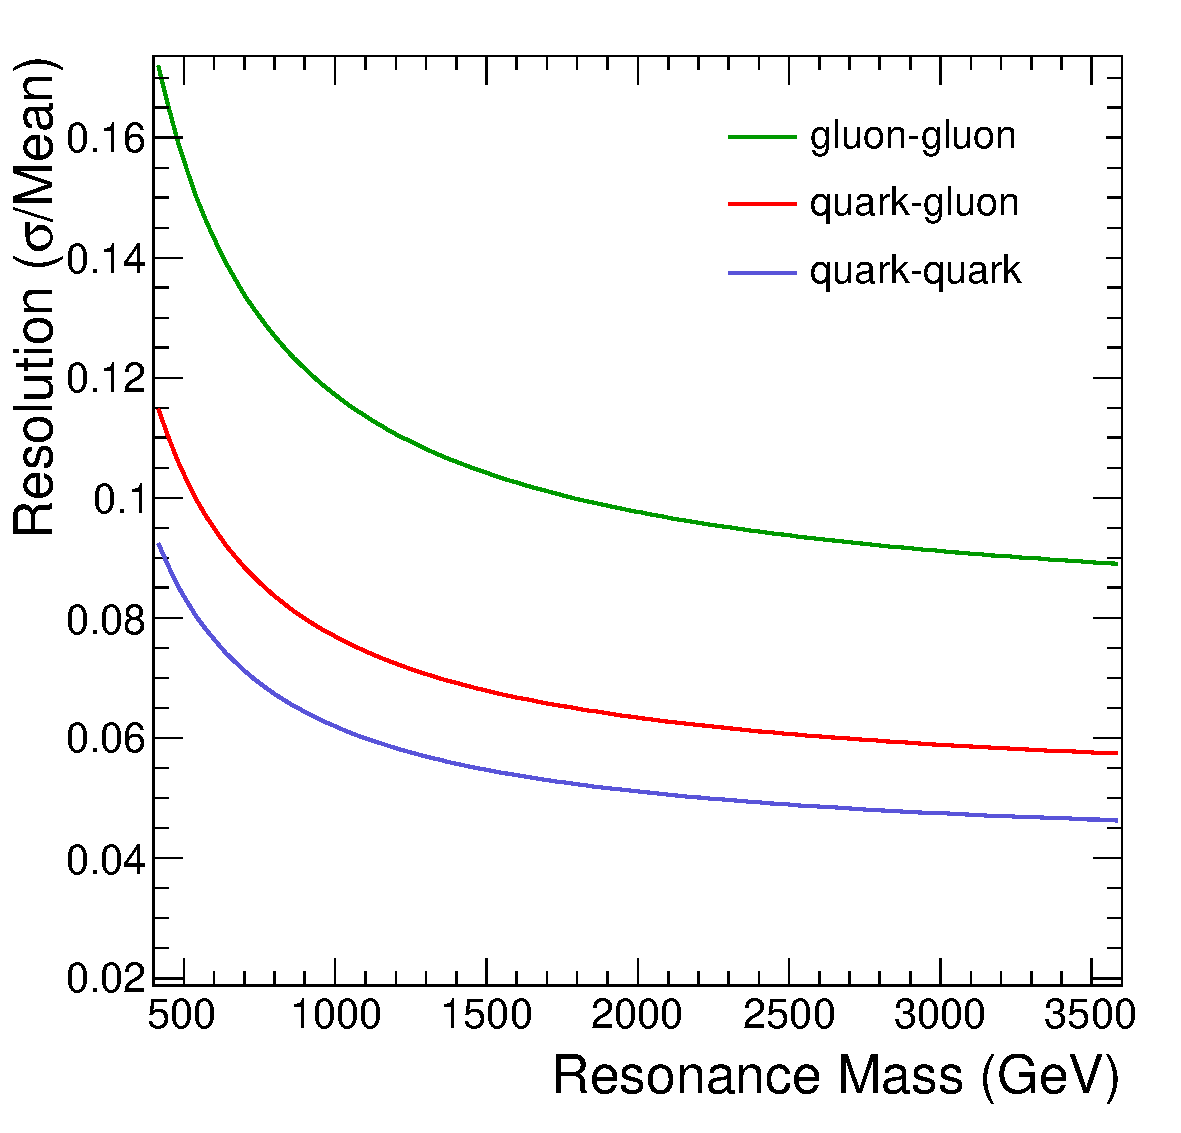
\includegraphics[width=\textwidth]{Figures/Comp_resolution_Color.pdf}
     \caption{The fractional width of the Gaussian core of the response distribution 
     as a function of resonance mass from CMS detector simulations of 
      $qq$, $qg$ and $gg$ dijet resonances.  }
    \label{resolution}
  \end{center}
\end{figure}

Fig.~\ref{shape} shows the simulated signal of excited quarks.
The resonance shape at resonance masses of $M=0.5$,$0.7$, $1.2$, $2.0$ and $3.5$
TeV were obtained from simulation.
We obtain the resonance shapes at intermediate masses via an 
interpolation technique~\cite{CMS_AN_2009-070}. For example the $1.5$ TeV
shape shown in Fig.~\ref{shape} comes from interpolation. The interpolation 
technique
has been checked by doing a wider interpolating between $M=0.7$ and $2.0$ TeV to get the $1.2$ TeV resonance
and comparing that with the actual simulation, and the shapes were the same. 
We use the resonance shapes from our interpolation technique to calculate the cross 
section upper limit at any resonance mass.

\begin{figure}[hbt]
  \begin{center}
     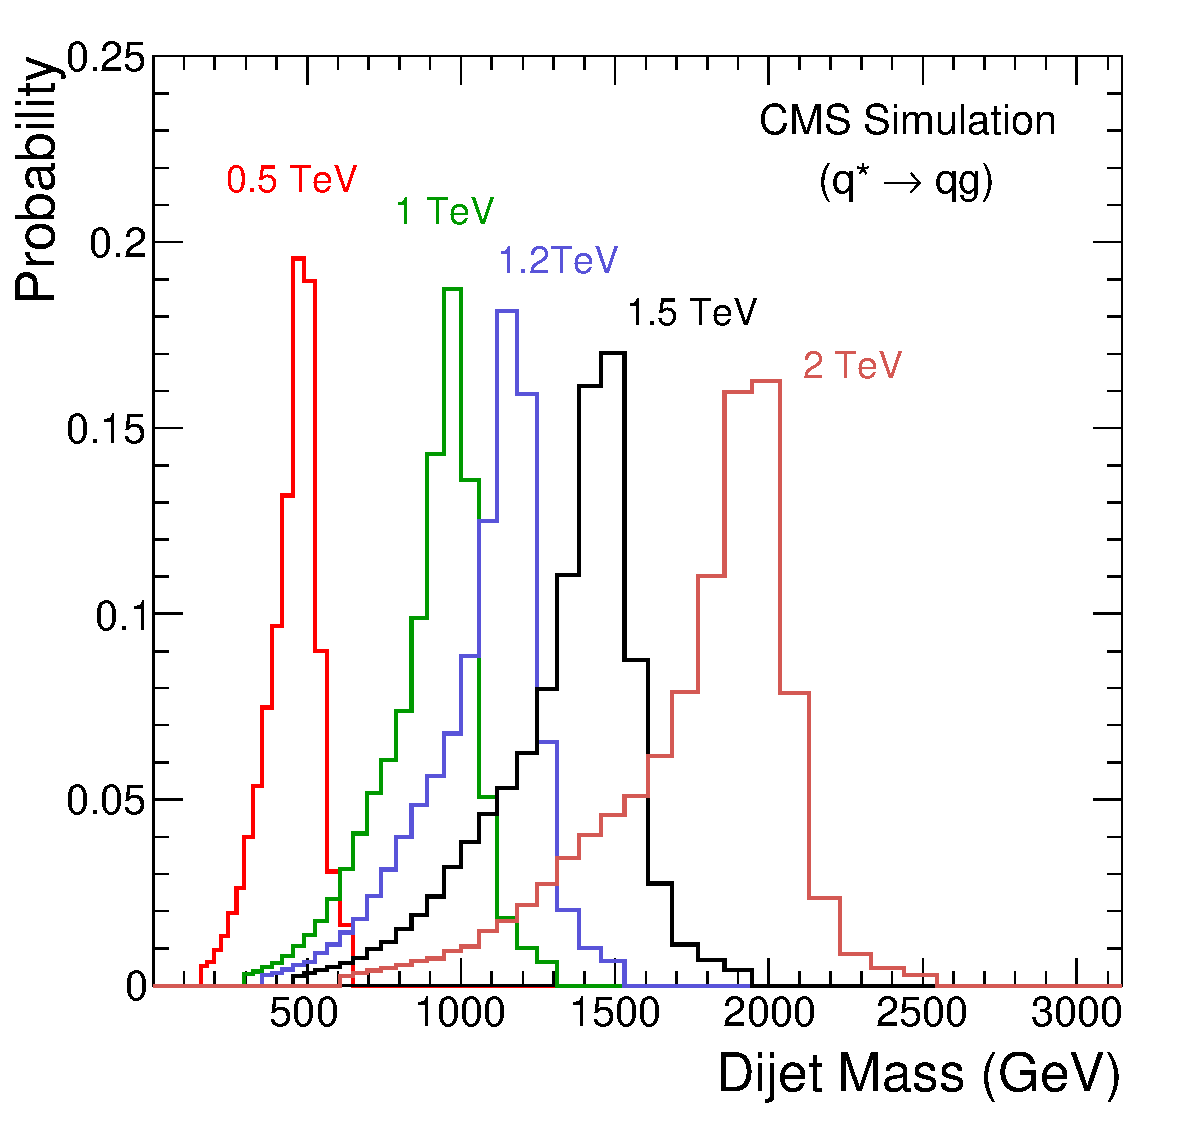
\includegraphics[width=\textwidth]{Figures/Shapes_qg.pdf}
     \caption{$qg$ resonance shapes at various resonance masses coming
     from excited quark simulation at resonance masses in TeV of 
     $0.5$ (red), $0.7$ (green), $1.2$ (blue), $2.0$ (red) and $3.5$ (not shown) and interpolation
     at the example mass of $1.5$ TeV (black).}
    \label{shape}
  \end{center}
\end{figure}

Fig.~\ref{signal_calo} shows the differential 
cross section of excited quark signals as a function of dijet mass 
superimposed on the plot of the dijet mass data with background fit. 
Fig.~\ref{signal_calo} also shows the 
differential cross section of string resonance signals. We model the
string resonance line shape using the excited quark shape since 
string resonances decay predominantly to a
quark and a gluon (see appendix~\ref{appString}) like the excited 
quark. Fig.~\ref{signal_calo} demonstrates that the expected string 
resonance cross section is large, much greater than our measured data.
%The fractional difference between the data and the smooth
%background fit is compared to 
%simulated excited quark resonance signals in Fig.~\ref{fract_signal}, and
%to string resonance signals in Fig.~\ref{fract_signal_string}.  Note 
%the vertical scales are different in Fig.~\ref{fract_signal} and 
%Fig.~\ref{fract_signal_string}.  
In Fig.~\ref{DataOverFit_calo} we show the ratio
between the data and the fit compared to simulated signals for both excited
quarks and string resonances.

\begin{figure}[hbt]
  \begin{center}
     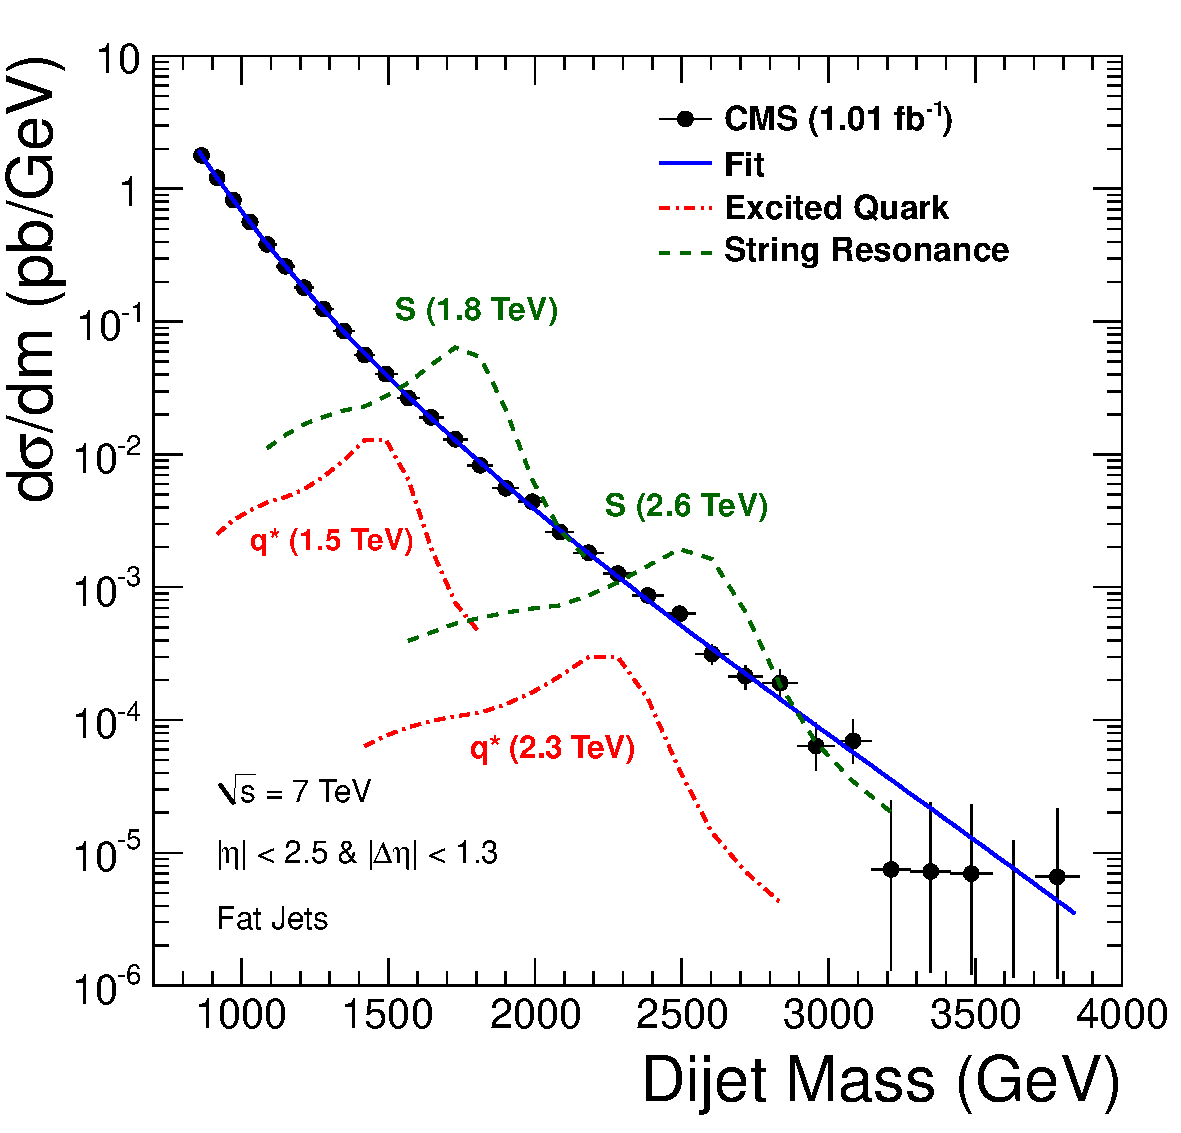
\includegraphics[width=\textwidth]{Figures/DijetMass_withSignal_fat.pdf}
     \caption{The dijet mass distribution for fat jets(points) compared to a smooth
     background fit (blue solid curve) and to a simulation of
     excited quarks (red dot-dashed curves) and string resonances (green dashed
     curves) in the CMS 
     detector.}
    \label{signal_fat}
  \end{center}
\end{figure}

\begin{figure}[hbt]
  \begin{center}
     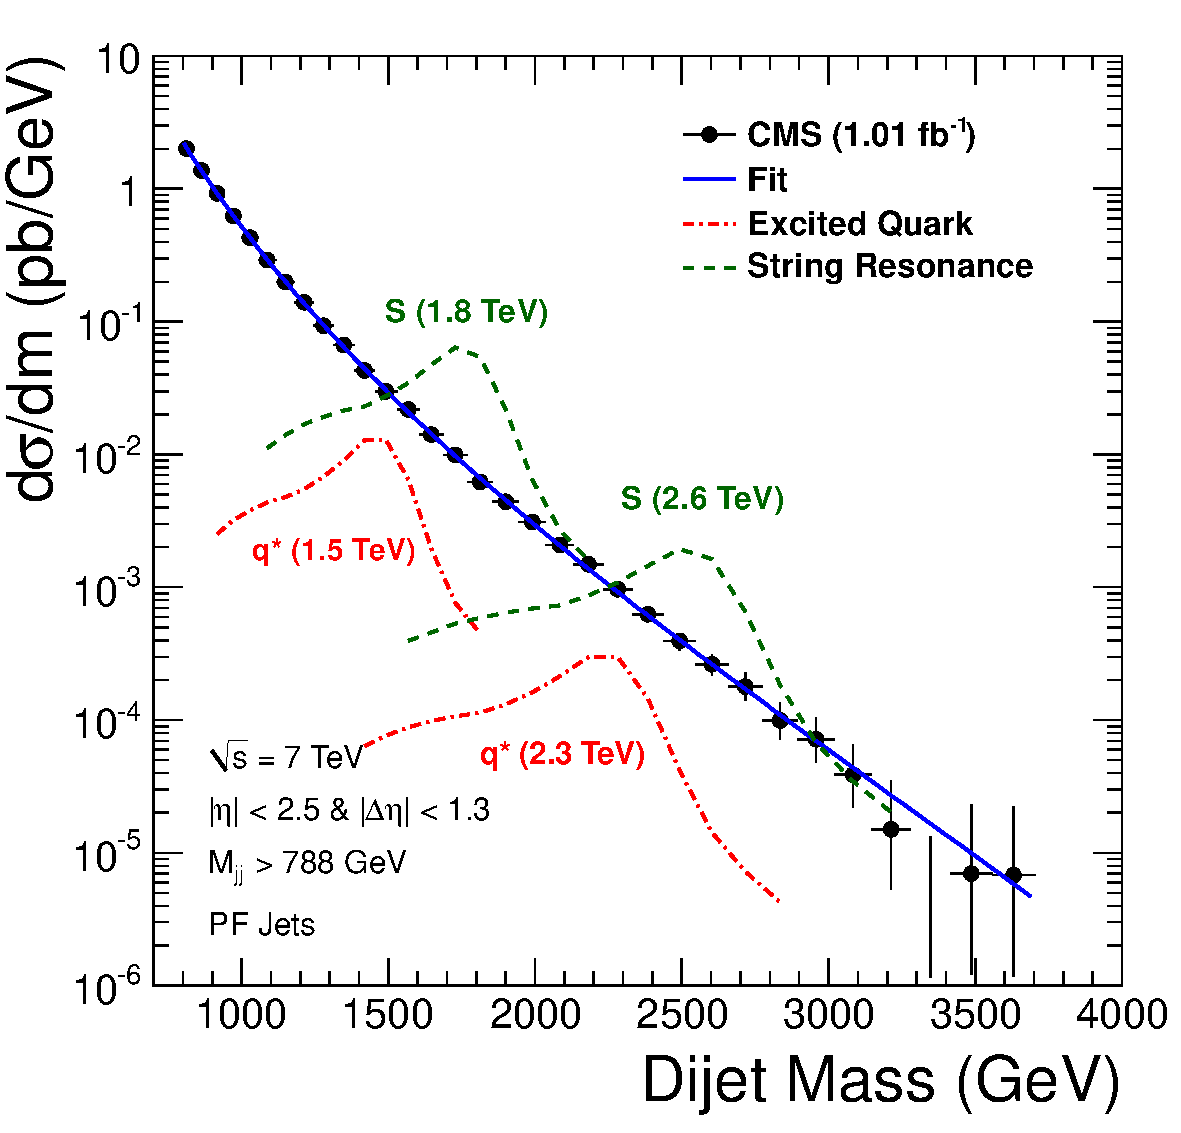
\includegraphics[width=\textwidth]{Figures/DijetMass_withSignal_pf.pdf}
     \caption{The dijet mass distribution for pf jets(points) compared to a smooth
     background fit (blue solid curve) and to a simulation of
     excited quarks (red dot-dashed curves) and string resonances (green dashed
     curves) in the CMS 
     detector.}
    \label{signal_pf}
  \end{center}
\end{figure}

\begin{figure}[hbt]
  \begin{center}
     \includegraphics[width=\textwidth]{Figures/DijetMass_withSignal_calo.pdf}
     \caption{The dijet mass distribution for calo jets(points) compared to a smooth
     background fit (blue solid curve) and to a simulation of
     excited quarks (red dot-dashed curves) and string resonances (green dashed
     curves) in the CMS 
     detector.}
    \label{signal_calo}
  \end{center}
\end{figure}

%\begin{figure}[hbt]
%  \begin{center}
%     \includegraphics[width=\textwidth]{Figures/Fract_change_withsignal.pdf}
%     \caption{ The fractional difference between the dijet mass distribution (points) and a smooth
%background fit (dashed line) is compared to simulations of excited quark signals in the CMS
%detector (dot-dashed red curves).}
%    \label{fract_signal}
%  \end{center}
%\end{figure}

%\begin{figure}[hbt]
%  \begin{center}
%     \includegraphics[width=\textwidth]{Figures/Fract_change_withsignal_string.pdf}
%     \caption{ The fractional difference between the dijet mass distribution (points) and a smooth
%background fit (dashed line) is compared to a simulation of a string resonance signal in the CMS
%detector (dashed green curve).}
%    \label{fract_signal_string}
%  \end{center}
%\end{figure}

\begin{figure}[hbt]
  \begin{center}
     \includegraphics[width=\textwidth]{Figures/data_over_fit_fat.pdf}
     \caption{ The ratio between the dijet mass distribution (points) and a smooth
background fit (dashed line) for fat jets is compared to a CMS detector simulation of an excited quark signal (dashed red curve).}
    \label{DataOverFit_fat}
  \end{center}
\end{figure}

\begin{figure}[hbt]
  \begin{center}
     \includegraphics[width=\textwidth]{Figures/data_over_fit_pf.pdf}
     \caption{ The ratio between the dijet mass distribution (points) and a smooth
background fit (dashed line) for pf jets is compared to a CMS detector simulation of an excited quark signal (dashed red curve).}
    \label{DataOverFit_pf}
  \end{center}
\end{figure}

\begin{figure}[hbt]
  \begin{center}
     \includegraphics[width=\textwidth]{Figures/data_over_fit_calo.pdf}
     \caption{ The ratio between the dijet mass distribution (points) and a smooth
background fit (dashed line) for calo jetsis compared to a CMS detector simulation of an excited quark signal (dashed red curve).}
    \label{DataOverFit_calo}
  \end{center}
\end{figure}

\clearpage

\subsection {Setting Cross Section Upper Limits}

For setting upper limits on dijet resonance cross section, before accounting for systematic uncertainties,
we begin with a Bayesian formalism with uniform prior for the cross section.
The binned likelihood, $L$, as a function of a constant $\alpha$ can be written as:
\\
\begin{equation}
L = \prod_{i} \frac{\mu_{i}^{n_{i}}e^{-\mu_{i}}}{n_{i}!}
\end{equation}
\\
where
\\
\begin{equation}
\mu_{i} = \alpha N_{i}(S) + N_{i}(B),
\end{equation}
\\
$n_{i}$ is the measured number of events in the $i^{th}$ dijet mass bin, $N_{i}(S)$ is the number of events from the signal in the $i^{th}$ dijet mass bin,
$\alpha$ is a constant to scaling the signal amplitude, and $N_{i}(B)$ is the number of expected events from background in the $i^{th}$ dijet mass bin.
We consider that the QCD background is fixed by the best $Signal+QCD$ fit to the data points and it gives the expected number of background event in the $i^{th}$
dijet mass bin, $N_{i}(B)$. The number of signal events in the $i^{th}$ dijet mass bin, $N_{i}(S)$, comes from an interpolation technique.
The signal range is chosen to be from $0.3\cdot M_{Res}$ to $1.3\cdot M_{Res}$, an interval which contains nearly all the resonance
line shape.
We assume a flat prior in $\alpha$, which is the same as a flat prior in the resonance cross section.  With this assumption
the likelihood normalized to unity is equivalent to a posterior probability density, and can be used to set limits.  
We calculate the posterior probability density as a function of signal cross section for resonances with 
mass from $0.6$ TeV to $3.3$ TeV in $0.1$ TeV steps.  Example likelihoods are shown in the appendix of  
AN-2010/108-v14 dated October 20, 2010 for the 3 pb$^{-1}$ dataset.
The 95\% confidence level upper limit $\sigma_{95}$ is calculated from the posterior probability density $P_{POST}$ as follows:

\begin{equation}
\frac{\int_{0}^{\sigma_{95}} P_{POST}(\sigma)d\sigma}{\int_{0}^{\infty} P_{POST}(\sigma)d\sigma} = 0.95
\end{equation}

%In Fig.~\ref{Likelihood}, Likelihood distribution at $0.7$ GeV resonance masses for $qg$ resonances are illustrated. The likelihood distributions 
%for resonance mass from $0.5$ TeV to $1.5$ TeV in $0.1$ TeV step can be seen in Appendix X.
%
%\begin{figure}[!ht]
%  \begin{center}
%    \includegraphics[width=0.55\textwidth]{Figures/Likelihood_700GeV.pdf}
%    \caption{Likelihood Distribution with statistical error only.}
%    \label{Likelihood}
%  \end{center}
%\end{figure}


We present the 95\% CL upper limit on dijet resonance cross section in 
Fig.~\ref{Limit_statonly_calo} including only statistical uncertainties. 
Quark-quark, quark-gluon, and gluon-gluon 
resonances are shown separately. The limits have small wiggles 
corresponding to structures in the data and the width of the
resonance line shape.  
The limits are also tabulated numerically in table~\ref{tabStatLimit_calo}. 
%At the highest resonance mass shown,
%2.6 TeV, the limits have a value of between 4 and 6 events. This corresponds to 
%the few events observed in the tail of the dijet mass distribution that are 
%still within the resonance line shape.  
%In prior analysis versions, where there were no events 
%at high dijet mass, we have shown explicitly that the limit plateaus at exactly 3 
%events, corresponding to 0 events observed.  


\subsection {Limit Setting with Roostat}

Until the AN-2010/018-v15, we made our own code to set limit based on a Bayesian method
fitting the data in our large variable sized bins with the data assigned to the center of the bin. 
In that method the data point was simply fit by a parameterization.
From now on we use Roostat to impliment the Bayesian method, since it's the official tool for statistics
now at CMS. Roostat is a statistical tool built on top of RooFit. In the new method the parameterization
is a density function which is integrated over the bin used to find the value within the bin. In the new
method the bin size is very fine, 1 GeV. 
%Using old method 
%and new method basically produce almost same result as you see in Fig~\ref{Limit_statonly_old_new}.
%The small difference is due to the differences in the fit when integrating the density over fine
%bins in the new method versus using the bin center in a fit with coarse variable bins in the old method.
%We verified for a previous dataset that when shrinking the coarse bins in the old method the two methods 
%converged towards the same result.
We fit the data after we make the dijet mass histogram from the trigger cut to 5 TeV with bin size
1 GeV in new method. 
%The 838 GeV lower edge of the dijet mass histogram comes from our dijet mass cut for more
%than 99.8\% trigger
%efficiency. 
The 5 TeV upper edge on dijet mass histogram allows us to use data up to that point to calculate
limits safely up to a resonance mass of 4 TeV. Once we get the background fit we follow the process that we descibed in previous section.
%Fig~\ref{Limit_statonly_old_new} shows both the new method using our Bayesian calculator, which has been
%constructed to permit fast and effective integrations necessary to include the systematics later, and also
%the results using the "out of the box" MCMC calculator, which is too slow to include systematics.  The results
%from our calculator agree almost exactly with the MCMC calculator.

%\begin{figure}[!ht]
%  \begin{center}
%    \includegraphics[width=\textwidth]{Figures/stat_limit_compare_old_new.pdf}
%    \caption{Dijet resonance sensitivity with statistical errors only. The 95\% C.L.
%      upper limit on cross section is compared to the cross section for old and new
%      methods. This sensitivity does not contain estimates of the systematic uncertainties.
%      Result from MCMC is also presented.}
%    \label{Limit_statonly_old_new}
%  \end{center}
%\end{figure}

\begin{figure}[!ht]
  \begin{center}
    \includegraphics[width=\textwidth]{Figures/c_xs_stat_fat.pdf}
    \caption{Dijet resonance sensitivity with statistical errors only for fat jets. The 95\% C.L. upper limit on cross section 
    is compared to the cross section for various resonance models.
This sensitivity does not contain estimates of the systematic uncertainties.}
    \label{Limit_statonly_fat}
  \end{center}
\end{figure}

\begin{figure}[!ht]
  \begin{center}
    \includegraphics[width=\textwidth]{Figures/c_xs_stat_pf.pdf}
    \caption{Dijet resonance sensitivity with statistical errors only for pf jets. The 95\% C.L. upper limit on cross section 
    is compared to the cross section for various resonance models.
This sensitivity does not contain estimates of the systematic uncertainties.}
    \label{Limit_statonly_pf}
  \end{center}
\end{figure}

\begin{figure}[!ht]
  \begin{center}
    \includegraphics[width=\textwidth]{Figures/c_xs_stat_calo.pdf}
    \caption{Dijet resonance sensitivity with statistical errors only for calo jets. The 95\% C.L. upper limit on cross section 
    is compared to the cross section for various resonance models.
This sensitivity does not contain estimates of the systematic uncertainties.}
    \label{Limit_statonly_calo}
  \end{center}
\end{figure}

%The procedure used in this note dates
%from one used by the CDF collaboration in Tevatron run I~\cite{Abe:1995jz,Abe:1997hm}, which was superseded in CDF run II~\cite{Aaltonen:2008dn} by a
% more fully
%Bayesian treatment of nuisance parameters. The newer CDF method
%(implemented in code by Ken Hatakeyama) gives a cross section upper
%limit which is roughly 10\% better than that in this note, presumably due
%to better treatment of the systematics, as discussed in the next section. 

%We have checked this procedure with independent software written for CDF by one of us (Ken Hatakeyama). 
%The CDF software gives a cross section upper limit that is pretty close, roughly 10\% better (smaller) 
%than ours, and we have not yet understood this small difference. We have also used the CDF software to 
%modify the basic limit setting method that we used, using a profile likelihood (posterior probability density).  
%The profile likelihood allows the background parameters to vary at every signal cross section point in the 
%likelihood, instead of fixing the background at the best $Signal+background$ fit. We note that CDF used the
%profile likelihood method in run 2~\cite{Aaltonen:2008dn}, and used the method of fixing the background at the best $Signal+background$ fit
%in run 1~\cite{Abe:1997hm}.  The resulting change between the two different methods in the limit for our dataset is small, 
%increasing by roughly 10-20\% at low masses and yielding in the end a very
%similar limit to the default machinery we use for limits.  
%More work needs
%to be done to incorporate the systematics into the profile likelihood 
%machinery, and to integrate the smooth operation of that machinery with our 
%personnel, before we can effectively use it to set limits.  We are encouraged 
%by the small difference between the two methods compared to our total 
%systematics described in the next section.

%\begin{figure}[!ht]
%  \begin{center}
%    \includegraphics[width=0.7\textwidth]{Figures/DijetMassLimitsProfileLikelihood}
%    \caption{Changes in the 95\% CL upper limits on the $qg$ resonance
%      cross section as a function of resonance masses when the profile
%      likelihood is used, compared to the case in which the background
%      parameters are fixed at the best $Signal+background$ fit. 
%      Analysis done independently with statistics software from CDF (see text).}
%    \label{LimitsProfileLikelihood}
%  \end{center}
%\end{figure}




\begin{table}[htbH]
\centering
\large
\begin{tabular}{|c|c|c|c|}\hline
Mass   &  \multicolumn{3}{c|}{95\% C.L. $\sigma\cdot B$ (pb) Stat. Err. Only}\\
 ($TeV$) & quark-quark       & quark-gluon  & gluon-gluon\\ \hline
1.0 & 0.98117 & 1.12380 & 1.71707 \\
1.1 & 0.71763 & 0.85015 & 1.30642 \\
1.2 & 0.66727 & 0.72977 & 1.05537 \\
1.3 & 0.46010 & 0.51269 & 0.77611 \\
1.4 & 0.26575 & 0.31458 & 0.49823 \\
1.5 & 0.22164 & 0.25654 & 0.38314 \\
1.6 & 0.19445 & 0.21768 & 0.31132 \\
1.7 & 0.17629 & 0.19703 & 0.28691 \\
1.8 & 0.11266 & 0.13608 & 0.20560 \\
1.9 & 0.10556 & 0.12224 & 0.17301 \\
2.0 & 0.11733 & 0.13513 & 0.18825 \\
2.1 & 0.09512 & 0.11829 & 0.16983 \\
2.2 & 0.08687 & 0.10578 & 0.14615 \\
2.3 & 0.09074 & 0.10945 & 0.14813 \\
2.4 & 0.08861 & 0.10462 & 0.14225 \\
2.5 & 0.07426 & 0.08945 & 0.12509 \\
2.6 & 0.05097 & 0.06451 & 0.08956 \\
2.7 & 0.03893 & 0.04842 & 0.06593 \\
2.8 & 0.03540 & 0.04219 & 0.05619 \\
2.9 & 0.02945 & 0.03485 & 0.04653 \\
3.0 & 0.02126 & 0.02569 & 0.03514 \\
3.1 & 0.01452 & 0.01840 & 0.02553 \\
3.2 & 0.00987 & 0.01305 & 0.01857 \\
3.3 & 0.00774 & 0.01016 & 0.01421 \\
3.4 & 0.00686 & 0.00892 & 0.01235 \\
3.5 & 0.00644 & 0.00820 & 0.01139 \\
3.6 & 0.00623 & 0.00782 & 0.01049 \\
3.7 & 0.00605 & 0.00753 & 0.00966 \\
3.8 & 0.00581 & 0.00721 & 0.00923 \\
3.9 & 0.00540 & 0.00672 & 0.00836 \\
4.0 & 0.00494 & 0.00621 & 0.00776 \\
4.1 & 0.00461 & 0.00578 & 0.00704 \\
\hline
\end{tabular}
\caption{As a function of resonance mass we list our 95\% C.L. upper limit on
cross section times branching ratio for narrow resonances originating from
quark-quark, quark-gluon and gluon-gluon pairs of partons, 
including statistical errors only for wide jets.}
\label{tabStatLimit_calo}
\end{table}

\clearpage

\begin{table}[htbH]
\centering
\large
\begin{tabular}{|c|c|c|c|}\hline
Mass   &  \multicolumn{3}{c|}{95\% C.L. $\sigma\cdot B$ (pb) Stat. Err. Only}\\
 ($TeV$) & quark-quark      & quark-gluon  & gluon-gluon\\ \hline
1.00 & 0.85831 & 1.02293 & 1.72368 \\
1.10 & 0.60046 & 0.75330 & 1.23105 \\
1.20 & 0.56792 & 0.65473 & 0.98512 \\
1.30 & 0.48672 & 0.55968 & 0.86245 \\
1.40 & 0.28078 & 0.36821 & 0.63206 \\
1.50 & 0.26078 & 0.30767 & 0.46226 \\
1.60 & 0.25040 & 0.29521 & 0.45434 \\
1.70 & 0.17622 & 0.21363 & 0.34735 \\
1.80 & 0.11481 & 0.14837 & 0.30056 \\
1.90 & 0.10280 & 0.12807 & 0.19840 \\
2.00 & 0.10238 & 0.12612 & 0.18930 \\
2.10 & 0.09798 & 0.12261 & 0.17560 \\
2.20 & 0.09835 & 0.12140 & 0.23845 \\
2.30 & 0.08913 & 0.11137 & 0.16376 \\
2.40 & 0.07353 & 0.09452 & 0.14190 \\
2.50 & 0.05916 & 0.07741 & 0.11798 \\
2.60 & 0.04798 & 0.06297 & 0.09646 \\
2.70 & 0.03922 & 0.05166 & 0.07991 \\
2.80 & 0.03171 & 0.04221 & 0.06448 \\
2.90 & 0.02635 & 0.03479 & 0.05331 \\
3.00 & 0.02153 & 0.02879 & 0.04484 \\
3.10 & 0.01628 & 0.02232 & 0.03558 \\
3.20 & 0.01204 & 0.01688 & 0.02701 \\
3.30 & 0.00934 & 0.01312 & 0.02069 \\
3.40 & 0.00803 & 0.01117 & 0.01730 \\
3.50 & 0.00753 & 0.01014 & 0.01530 \\
3.60 & 0.00709 & 0.00942 & 0.01417 \\
3.70 & 0.00645 & 0.00857 & 0.01251 \\
3.80 & 0.00581 & 0.00775 & 0.01097 \\
3.90 & 0.00524 & 0.00702 & 0.00976 \\
4.00 & 0.00487 & 0.00651 & 0.00890 \\
4.10 & 0.00459 & 0.00608 & 0.00816 \\
\hline
\end{tabular}
\caption{As a function of resonance mass we list our 95\% C.L. upper limit on
cross section times branching ratio for narrow resonances originating from
quark-quark, quark-gluon and gluon-gluon pairs of partons, 
including statistical errors only for PF jets.}
\label{tabStatLimit_pf}
\end{table}

\clearpage

\begin{table}[htbH]
\centering
\large
\begin{tabular}{|c|c|c|c|}\hline
Mass   &  \multicolumn{3}{c|}{95\% C.L. $\sigma\cdot B$ (pb) Stat. Err. Only}\\
 ($TeV$) & quark-quark      & quark-gluon  & gluon-gluon\\ \hline
1.00 & 0.93190 & 1.11411 & 1.89363 \\
1.10 & 0.69784 & 0.88578 & 1.51219 \\
1.20 & 0.42125 & 0.53369 & 0.97204 \\
1.30 & 0.39265 & 0.46737 & 0.76679 \\
1.40 & 0.28961 & 0.37591 & 0.64415 \\
1.50 & 0.28572 & 0.32622 & 0.48846 \\
1.60 & 0.25762 & 0.31199 & 0.49229 \\
1.70 & 0.19334 & 0.24708 & 0.41693 \\
1.80 & 0.11484 & 0.16159 & 0.30167 \\
1.90 & 0.11042 & 0.13607 & 0.20965 \\
2.00 & 0.13905 & 0.15910 & 0.21740 \\
2.10 & 0.12875 & 0.16227 & 0.24188 \\
2.20 & 0.09711 & 0.12948 & 0.21242 \\
2.30 & 0.08848 & 0.11087 & 0.16605 \\
2.40 & 0.06886 & 0.09347 & 0.15335 \\
2.50 & 0.04914 & 0.06895 & 0.11706 \\
2.60 & 0.03912 & 0.05323 & 0.08715 \\
2.70 & 0.03200 & 0.04371 & 0.07215 \\
2.80 & 0.02706 & 0.03609 & 0.05802 \\
2.90 & 0.02291 & 0.03040 & 0.04732 \\
3.00 & 0.01852 & 0.02525 & 0.04111 \\
3.10 & 0.01387 & 0.01957 & 0.03248 \\
3.20 & 0.01048 & 0.01504 & 0.02480 \\
3.30 & 0.00842 & 0.01190 & 0.01924 \\
3.40 & 0.00734 & 0.01015 & 0.01605 \\
3.50 & 0.00682 & 0.00909 & 0.01381 \\
3.60 & 0.00653 & 0.00855 & 0.01263 \\
3.70 & 0.00608 & 0.00798 & 0.01152 \\
3.80 & 0.00560 & 0.00737 & 0.01055 \\
3.90 & 0.00509 & 0.00674 & 0.00940 \\
4.00 & 0.00482 & 0.00629 & 0.00839 \\
4.10 & 0.00453 & 0.00589 & 0.00770 \\
\hline
\end{tabular}
\caption{As a function of resonance mass we list our 95\% C.L. upper limit on
cross section times branching ratio for narrow resonances originating from
quark-quark, quark-gluon and gluon-gluon pairs of partons, 
including statistical errors only for calo jets.}
\label{tabStatLimit_fat}
\end{table}

\clearpage


\section {Systematic Uncertainties on the Search}

The source of systematic uncertainties are considered as following:
\begin{itemize}
\item Jet Energy Scale (JES)
\item Jet Energy Resolution (JER) 
\item Choise of Background Parametrization
\item Luminosity
\end{itemize}
Our procedure to evaluate the first three is to use a smooth fit to the 
QCD background as a data sample, and find the cross section upper limits for 
this data sample before and after systematic shifts, described below. 

\subsection{Jet Energy Scale (JES)} 
The uncertainty on the JES that is important for this analysis
is the uncertainty on how well the dijet resonance simulation models the jet energy scale of real jets.
If the simulation produces jets with too high a response, then the true position of the expected resonance
peak for that resonance mass would really be at lower mass than predicted by the simulation.
We assume that the uncertainty on JES is roughly $\pm10\%$ and test the sensitivity of our 
analysis to a shift in the resonance signal by 10\%. Shifting the resonance 10\% lower in dijet mass 
gives more background from QCD and finding the resonance signal is harder.\\
The left plot in Fig.~\ref{JES} shows smooth cross section limit without systematics and with systematics on JES uncertainty for $qg$ resonance. 
To get smooth cross section limit curve, expected events from background, $N_{i}(B)$, which is smooth and comes from fit function are considered 
as measurement number of events, $n_{i}$, in the $i-th$ dijet mass bin. 
Fractional change between smooth limits are illustrated separately at right plot of Fig.~\ref{JES}. The 
systematic uncertainty decreases with resonance mass primarily because we are setting limits at the
edge of the region with real data, and the uncertainty is very sensitive to whether any data events are
expected from the background: if there is no background, there is no change in the limit with JES uncertainty.
This systematic has increased with luminosity at high resonance mass, and we expect that this systematic 
uncertainty will continue to increase as we get more data.

\begin{figure}[!ht]
  \begin{center}
%   \includegraphics[width=0.45\textwidth]{Figures/Limit_Comparison_JES_Systematic.pdf}
   \includegraphics[width=0.45\textwidth]{Figures/Fractional_Change_JES_All.pdf}
    \caption{ 
%\textit{Left plot}: Comparison of smoothed cross section limit with and without JES systematic uncertainty.
%\textit{Right plot}:
Fractional change on limit with JES systematic uncertainty.}
    \label{JES}
  \end{center}
\end{figure}
\clearpage

\subsection{Jet Energy Resolution (JER)}

JetMET recommends a resolution systematic of 10\% which is supported by the first measurements
of the RMS resolution in data using the dijet $p_T$ asymmetry method~\cite{PAS_JME_10-003}.
The tails of the resolution function are in good agreement between data and MC~\cite{CMS_AN_2010/134}.
This same dijet asymmetry method with a varying cut on the 3rd jet pt constrains the differences in 
radiation between the data and MC~\cite{CMS_AN_2010/134}, and thereby constrains differences in MC 
modelling of the resonance shape due to radiation to not be a big effect.
We assume that the uncertainty on JER is roughly $\pm10\%$ and the signal is being smeared 
with a Gaussian that increases the core resolution by 10\%. A comparison of resonace shapes are shown in
Fig.\ref{conv_shape}.

\begin{figure}[!ht]
  \begin{center}
     \includegraphics[width=0.3\textwidth]{Figures/Resonace_Shape_Convoluted_qq_1200.pdf}
       \includegraphics[width=0.3\textwidth]{Figures/Resonace_Shape_Convoluted_qg_1200.pdf}
        \includegraphics[width=0.3\textwidth]{Figures/Resonace_Shape_Convoluted_gg_1200.pdf}
         \includegraphics[width=0.3\textwidth]{Figures/Resonace_Shape_Convoluted_qq_1200_2.pdf}
          \includegraphics[width=0.3\textwidth]{Figures/Resonace_Shape_Convoluted_qg_1200_2.pdf}
           \includegraphics[width=0.3\textwidth]{Figures/Resonace_Shape_Convoluted_gg_1200_2.pdf}
    \caption{Resonance shape comparison after convolution at $0.5$ GeV (top) and $1.2$ TeV (bottom).}
    \label{conv_shape}
  \end{center}
\end{figure} 

Dijet mass core resolution of the resonance signal as a function of resonance
mass was illustrated in Fig.~\ref{resolution}. The resolution is calculated as 
$Sigma/Mean$ which are obtained from Gaussian fit of dijet mass distribution.
The fractional change on Limit with JER systematic is illustrated 
in Fig.~\ref{JER}. Effect of resolution uncertainty on limit is small.

\begin{figure}[!ht]
  \begin{center}
    \includegraphics[width=0.6\textwidth]{Figures/Fractional_Change_JER_All.pdf}
    \caption{Fractional change on limit with JER systematic uncertainty.}
    \label{JER}
  \end{center}
\end{figure}

\clearpage


\subsection{Background Parameterization}
We considered others functional forms to parametrize the QCD background as discussed in section~\ref{sectionParam}. 
%The only form that is a good fit to our data is Alternate Fit A with 4 parameters.
We have determined the affect on the limit, for a smoothed data sample, of changing 
from our default fit to Alternate Fit A with 4 parameters.  The smooth positive envelope of the 
fractional difference is shown in Fig.~\ref{Background}.  The shallow peaking of the systematic 
is because the systematic shift is small at very low resonance mass where there are lots of events
to constrain the background and give a good fit. Then, as the resonance mass increases, the fit is more
poorly contrained by fewer events and the systematic increases. Finally. at the highest resonance 
masses there is no background, and the systematic must decrease again.
%As a result, 
%the systematic peaks at a resonance mass close to the edge of our data where there is background, but
%the background is poorly constrained by the few number of events expected. 

\begin{figure}[!ht]
  \begin{center}
%     \includegraphics[width=0.45\textwidth]{Figures/Fractional_Change_Background_comparison.pdf}
       \includegraphics[width=0.6\textwidth]{Figures/Fractional_Change_Background_All.pdf}
    \caption{ Fractional change in the limit for the three resonance types when finding the background 
     using an alternate fit function.}
    \label{Background}
  \end{center}
\end{figure}

\subsection{Total Uncertainty}
We determine $1\sigma $ change for each systematic uncertainty in signal that we can discover or exclude. In
addition to the sources already mentioned, we include an uncertainty of 11\%.

To find total 
systematics, we add these $1\sigma $ changes in quadrature. 
The individual and total systematic uncertainties 
as a function 
of resonance mass are shown in Fig.~\ref{uncer}. 
Absolute uncertainty in each resonance mass is calculated as 
total fractional systematic 
uncertainty multiplied by upper cross section limit. 

\begin{figure}[!h]
  \begin{center}
         \includegraphics[width=0.45\textwidth]{Figures/Fractional_Uncer.pdf}
     \includegraphics[width=0.45\textwidth]{Figures/Fract_Uncer_All.pdf}
    \caption{ Fractional systematic uncertainties on resonance cross section.
    Left) Individual uncertainties are shown along with the total for $qg$ resonances.
    Right) Total fractional uncertainties are compared for $qq$, $qg$, and
    $gg$ resonances.}
    \label{uncer}
  \end{center}
\end{figure}


\subsection{Incorporating Systematics in the Limit}

We convolute the posterior probability density with a Gaussian for each resonance mass. The equation of convolution is 

\begin{equation}
P_{POST}(\sigma) = \int_{0}^{\infty} P_{POST}(\sigma^{\prime}) G(\sigma, \sigma^{\prime}) d\sigma^{\prime}
\label{eqConvolution}
\end{equation}

Where $P_{POST}(\sigma^{\prime})$ is the posterior probability density at signal cross section $\sigma^{\prime}$,
and  $G(\sigma, \sigma^{\prime})$ is the Gaussian probability from systematics to observe $\sigma$ if 
$\sigma^{\prime}$ is expected.  The width of the Gaussian is taken as 
the absolute uncertainty in each resonance mass, equal to the fractional uncertainty times the limit on the cross section. This
procedure, identical to what was done at CDF in run 1~\cite{Abe:1997hm}, 
This procedure was used in CDF Run I, but has since been superseded
in CDF Run II by a more appropriate Bayesian treatment of systematics,
implemented using some formalism described in Ref~\cite{CDF5305}. 
Our procedure conservatively assigns the same width to the Gaussian in units of pb at each point 
in the posterior probability density as a function of cross section.  This produces more smearing of the probability to higher
values of cross section than using a fractional uncertainty, which would give smaller Gaussian widths at lower cross section values,
and we think it better characterizes the overall uncertainty. The convoluted value $P_{POST}(\sigma)$ is normalized
to unit area over the range $0<\sigma<\infty$.
Posterior probability densities with systematic uncertainties are shown in Appendix~\ref{appLike}. 
Total posterior probability desnity including systematics is broader and gives a higher upper limit.


For most cases, where the posterior probability density including statistical uncertainties only 
peaks at cross section values of zero, the procedure used for convolution pushes the 
probability density away from zero, creating a peak in the probability at small cross section values 
after systematics that was not there before systematics.
This does not reflect more probability for a resonance at this cross section than zero
cross section, but rather is an artifact of the convolution procedure. The procedure assigns an appreciable 
absolute systematic even at zero cross section and does not permit smearing from unphysical 
negative cross section to positive cross section, which reduces the probability for zero cross section.
This may be an artifact of using Eq.~\ref{eqConvolution} to incorporate systematics instead of a fully 
Bayesian calculation.
Caution must be used in interpreting bumps in this probability density after systematics if they
were not present and significant before systematics.  
On the contrary, for a genuine resonance, which has
significant separation from zero cross section in the posterior probability density before systematics, 
the mean value of the cross section after systematics remains the same.


 We have checked that this procedure for incorporating systematics gives reasonable results compared 
with a method used by CDF in run II~\cite{Aaltonen:2008dn}.  We have been informed that the CDF 
run II method is closer to a true Bayesian incorporation of sytematic uncertainties than the 
method we used.  The CDF run II method gives roughly 
10\% lower cross section upper limits at all resonances masses after incorporating systematics than
the method we used. We conclude that the method we used is conservative.


Our 95\% CL upper limit with statistical uncertainties only and including stystematic 
uncertainties are shown separately in Fig.~\ref{limit_change} for qg resonances. 
The effects of systematics 
on the limit is also presented in Fig.~\ref{limit_change} as a fractional change in the limit for
all three resonance types.
We note that for both string resonances and excited quarks, the mass limits are reduced by only
0.1 TeV by including systematics.
%We note that at a resonance mass of 1.7 TeV the cross section upper limit increases by
%18\% after incorporating our conservative systematic uncertainties.
%This decreases the mass limit on string resonances by only 3\%, or $0.05$ TeV.
%The effect of systematics on our string resonance mass limit is small.

\begin{figure}[!ht]
  \begin{center}
     \includegraphics[width=0.48\textwidth]{Figures/Limit_Comparison_Systematic.pdf}
    \includegraphics[width=0.48\textwidth]{Figures/Fractional_Change_Limit_All.pdf}
    \caption{Left) Limits on qg resonances with and without all systematic uncertainties. 
    Right) Fractional change in the limit after including systematics.}
    \label{limit_change}
  \end{center}
\end{figure}

\clearpage

%\begin{figure}[!ht]
%  \begin{center}
%    \includegraphics[width=0.7\textwidth]{Figures/Limit_Comparison_Systematic.pdf}
%    \caption{Comparison of 95\% cross section limits with excited quark cross section. }
%    \label{limit_change}
%  \end{center}
%\end{figure}

%\vspace*{1.5cm}
%\begin{table}[htbH]
%\centering
%\large
%\begin{tabular}{|c|c|c|}\hline
%Mass   &  \multicolumn{2}{c|}{95\% C.L. $\sigma\cdot B$ (pb)}\\
% ($TeV$) &  Stat. Error Only & Including Systematic Uncer.\\ \hline
% 0.5     &  2402             & 3915   \\
% 0.6     &  1416             & 2333   \\
% 0.7     &  1254             & 2061   \\
% 0.8     &  1101             & 1620   \\
% 0.9     &   923             & 1281   \\
% 1.0     &   746             &  953   \\
% 1.1     &   654             &  797   \\
% 1.2     &   584             &  675   \\
% 1.3     &   542             &  610   \\
% 1.4     &   507             &  562   \\
% 1.5     &   481             &  522   \\
%\hline
%\end{tabular}
%\caption{As a function of excited quark mass we list our 95\% C.L. upper limit on
%cross section times branching ratio for narrow resonances of excited quark decaying to dijets}
%\end{table}





%\section{Expected and Observed Limits}

We have used the methodology described in this note and in a prior analysis~\cite{CMS_AN_2009-070} to 
determine our expected limits.  For the expected limits the PYTHIA MC
samples discussed previously were used for the background, but otherwise the analysis is the same 
as just described.  We form smooth background samples without fluctuations from a smooth fit
to the QCD data and use the number of events expected in each bin from this smooth fit to perform
the analysis. The expected limits on the cross section are compared to the observed limits in 
Fig.~\ref{limit_qg} and ~\ref{limit_qq}.

%The expected upper limits on the cross section are shown in Fig.~\ref{future_limit}
%compared to 7 models of resonance.   The mass limit expected for each model occurs where the expected
%upper limit on the cross section for the appropriate parton pair crosses the model cross section curve.
%These expected 95\% CL mass limits are plotted in Figure~\ref{future_mass_limit} as a function of integrated
%luminosity. The slope and functional form of the mass limit dependence
%on integrated luminosity strongly depends on the parton distributions involved in the process. The $E_6$ diquark
%process excluded mass limits curve vs. integrated luminosity is not linear like for $q^*$ and Colorons because
%the $E_6$ diquark cross section slope vs. resonance mass changes appreciably in the region $0.5$ to $3$ TeV.
%We have already surpassed the mass limit on string resonances set by the Tevatron, and 
%with 400 nb$^{-1}$ we expect to reach the mass limit of 870 GeV for excited quarks also from the Tevatron.



\begin{figure}[!ht]
  \begin{center}
    \includegraphics[width=\textwidth]{Figures/Limit_QG.pdf}
    \caption{The observed 95\% C.L. upper limits on the cross section for 
    quark-gluon resonances (blue points) is compared to the expected limits (green boxes)
    and to cross section predictions for string resonances (dot-dashed blue curve) and 
    excited quarks (dashed red curve) in the dijet channel. }
    \label{limit_qg}
  \end{center}
\end{figure}

\begin{figure}[!ht]
  \begin{center}
    \includegraphics[width=\textwidth]{Figures/Limit_QQ.pdf}
    \caption{The observed 95\% C.L. upper limits on the cross section for 
    quark-gluon resonances (blue points) is compared to the expected limits (green boxes)
    and to cross section predictions for string resonances (dot-dashed blue curve) and 
    excited quarks (dashed red curve) in the dijet channel.}
    \label{limit_qq}
  \end{center}
\end{figure}


%With 120 nb$^{-1}$ of data, our actual measured mass limit for string resonances, 
%$1.67$ TeV is in good agreement with the expected mass limits of $1.75$.  Our actual
%meaaured mass limit for excited quarks, $0.59$ TeV is slighly lower than the expected
%mass limit of $0.63$ TeV because of the single bin upward fluctuation in the data near
%$0.6$ TeV.  Converseley, our actual measured mass limit for axigluons and colorons, 
%$0.52$ TeV, is higher than our expected mass limit of $0.40$ TeV, because of 
%the downward fluctuation of the data around $0.5$ TeV.


%\begin{figure}[!ht]
%  \begin{center}
%     \includegraphics[width=0.48\textwidth]{Figures/Smooth_limit_including_sys_100nb.pdf}
%     \includegraphics[width=0.48\textwidth]{Figures/Smooth_limit_including_sys_300nb.pdf}
%     \includegraphics[width=0.48\textwidth]{Figures/Smooth_limit_including_sys_1pb.pdf}
%     \includegraphics[width=0.48\textwidth]{Figures/Smooth_limit_including_sys_10pb.pdf}
%     \includegraphics[width=0.48\textwidth]{Figures/Smooth_limit_including_sys_100pb.pdf}
%     \includegraphics[width=0.48\textwidth]{Figures/Smooth_limit_including_sys_1fb.pdf}
%    \caption{Model cross sections (curves) compared to the CMS expected upper 
%    limits (points) at 6 different integrated luminosities:
%    0.1,0.3, 1, 10, 100, and 1000 pb$^{-1}$.}
%    \label{future_limit}
%  \end{center}
%\end{figure}

%\begin{figure}[!ht]
%  \begin{center}
%     \includegraphics[width=\textwidth]{Figures/excluded_mass_limit.pdf}
%    \caption{Expected excluded mass limits at 95\% CL vs. integrated luminosity for
%    various various models.}
%    \label{future_mass_limit}
%  \end{center}
%\end{figure}


%%%%%%%%%%%%%%%%%%%%%%%%%%%%%%%%%%%%%%%%%%%%%%%%%%%%%%%%%%%%%%%%%%%%%%%%%%
%%%%%%%%%%%%%%%%%%%%%%%%%%%%%%%%%%%%%%%%%%%%%%%%%%%%%%%%%%%%%%%%%%%%%%%%%%
\clearpage{}
\section{Results}
\label{sec:results}
% ---- ---- ---- ---- ---- ---- ---- ---- ---- ---- ---- ---- ---- ---- ----
\par
The well-known formula for the extraction of  a cross section is:
\begin{equation}
\label{eq:xsec}
 \sigma = \frac{N^{\text{Sig}}}
               { A \, \epsilon \, {\cal{L}} }
\end{equation}
where $N^{\text{Sig}}$ is the number of extracted signal events,
$A$ is the signal acceptance corrected for the branching fraction,
$\epsilon$ is the efficiency for all requirements on 
the event selection, and ${\cal{L}}$ is the integrated luminosity.
Using the number of signal diboson events from 
table~\ref{table:FitTotalsAndComparisons} and efficiency $\times$ 
acceptance values from table~\ref{tab:signals}, we obtain the 
WW+WZ cross section values for each disjoint sub-sample as shown in 
table~\ref{tab:measuredCrossSection}
%%%%%%%%%%%%%%%%%%%%%%%%%%%%%
\begin{table}[h]
\begin{center}
  \begin{tabular}{l c}
    \hline  \hline
    Event category &  Measured cross section\\
    \hline
    $\mu jj$        &    $73.41 \pm 15.07$  pb\\
    $ejj$           &    $60.14 \pm 21.50$  pb\\   \hline 
    $\mu jj$,b-tag  &    $76.85 \pm 60.68$  pb\\
    $ejj$,b-tag     &    $22.71 \pm 49.27$  pb\\   \hline 
    Theory prediction~\cite{Campbell:2011bn} &  $65.6 \pm 2.2$ pb\\
    \hline  \hline
  \end{tabular}
\end{center}
\caption{\label{tab:measuredCrossSection}
The measured values of the sum of WW and WZ cross section in each disjoint sub-sample. 
The uncertainties include both statistical and systematic.}
\end{table}
%%%%%%%%%%%%%%%%%%%%%%%%%%%%%

Combining all four channels, we obtain:

WW+WZ cross section = 66.70 $\pm$ 11.74 pb.\\
[Breaking down the uncertainties: 66.70 $\pm$ 8.08 (stat) $\pm$ 8.52 (syst) pb]


We produce combined plots for electrons and muons in
Figs~\ref{fig:combinedNoBtag} and~\ref{fig:combinedWithBtag} for no $b$
tags and with $b$ tags, respectively.

\begin{figure}
\begin{center}
\includegraphics[width=0.45\textwidth]{figs/mjjfit_2jetsample/Diboson_Stacked_combined}
\includegraphics[width=0.45\textwidth]{figs/mjjfit_2jetsample/Diboson_Subtracted_combined}
\includegraphics[width=0.45\textwidth]{figs/mjjfit_2jetsample/Diboson_Pull_combined}
\end{center}
\caption{Combined results of both muons and electrons without btags}
\label{fig:combinedNoBtag}
\end{figure}

\begin{figure}
\begin{center}
\includegraphics[width=0.45\textwidth]{figs/mjjfit_2jetsample/Diboson_btag_Stacked_combined}
\includegraphics[width=0.45\textwidth]{figs/mjjfit_2jetsample/Diboson_btag_Subtracted_combined}
\includegraphics[width=0.45\textwidth]{figs/mjjfit_2jetsample/Diboson_btag_Pull_combined}
\end{center}
\caption{Combined results of both muons and electrons with btags}
\label{fig:combinedWithBtag}
\end{figure}


\subsection{Results including only non b-tag categories}
\label{sec:results2ch}
% ---- ---- ---- ---- ---- ---- ---- ---- ---- ---- ---- ---- ---- ---- ----
Including only non b-tag (both muon and electron) categories, we 
observe 2682 $\pm$ 339 (stat) $\pm$ 357 (syst) WW+WZ events, 
in agreement with the Standard Model expectation. 
This corresponds to a significance of $8.8~\sigma$ 
($7.8~\sigma$ in muon data and $4.4~\sigma$ in electron data) 
when computed using a simple likelihood 
ratio where the nuisance parameters are fixed to their nominal fit 
values in case of the null hypothesis. 
Using the profile likelihood ratio, where the nuisance parameters are 
allowed to vary also for the null hypothesis, the significance 
becomes $4.34~\sigma$ ($4.31~\sigma$ in muon data 
and $1.60~\sigma$ in electron data).


Combining results of muon and electron non b-tag categories, we obtain
the following result for cross section:
$\sigma = 68.89 \pm 8.71 \text{(stat)} \pm 9.70 \text{(syst)}  \pm 1.52 \text{(lumi)}$~pb, 
which is in agreement with the NLO prediction 
$65.6 \pm 2.2$~pb that includes $gg\to\text{WW}$ contribution.


%\section{Expected Limits}

We have used the methodology described in this note and in a prior analysis~\cite{CMS_AN_2009-070} to 
determine our expected limits with more integrated luminosity.  For the expected limits the PYTHIA MC
samples discussed previously were used for the background, but otherwise the analysis is the same 
as just described.  We form smooth samples background samples without fluctuations from a smooth fit
to the QCD data and use the number of events expected in each bin from this smooth fit to perform
the analysis.  The expected upper limits on the cross section are shown in Fig.~\ref{future_limit}
compared to 7 models of resonance.   The mass limit expected for each model occurs where the expected
upper limit on the cross section for the appropriate parton pair crosses the model cross section curve.
These expected 95\% CL mass limits are plotted in Figure~\ref{future_mass_limit} as a function of integrated
luminosity. The slope and functional form of the mass limit dependence
on integrated luminosity strongly depends on the parton distributions involved in the process. The $E_6$ diquark
process excluded mass limits curve vs. integrated luminosity is not linear like for $q^*$ and Colorons because
the $E_6$ diquark cross section slope vs. resonance mass changes appreciably in the region $0.5$ to $3$ TeV.
We have already surpassed the mass limit on string resonances set by the Tevatron, and 
with 400 nb$^{-1}$ we expect to reach the mass limit of 870 GeV for excited quarks also from the Tevatron.


%With 120 nb$^{-1}$ of data, our actual measured mass limit for string resonances, 
%$1.67$ TeV is in good agreement with the expected mass limits of $1.75$.  Our actual
%meaaured mass limit for excited quarks, $0.59$ TeV is slighly lower than the expected
%mass limit of $0.63$ TeV because of the single bin upward fluctuation in the data near
%$0.6$ TeV.  Converseley, our actual measured mass limit for axigluons and colorons, 
%$0.52$ TeV, is higher than our expected mass limit of $0.40$ TeV, because of 
%the downward fluctuation of the data around $0.5$ TeV.


\begin{figure}[!ht]
  \begin{center}
     \includegraphics[width=0.48\textwidth]{Figures/Smooth_limit_including_sys_100nb.pdf}
     \includegraphics[width=0.48\textwidth]{Figures/Smooth_limit_including_sys_300nb.pdf}
     \includegraphics[width=0.48\textwidth]{Figures/Smooth_limit_including_sys_1pb.pdf}
     \includegraphics[width=0.48\textwidth]{Figures/Smooth_limit_including_sys_10pb.pdf}
     \includegraphics[width=0.48\textwidth]{Figures/Smooth_limit_including_sys_100pb.pdf}
     \includegraphics[width=0.48\textwidth]{Figures/Smooth_limit_including_sys_1fb.pdf}
    \caption{Model cross sections (curves) compared to the CMS expected upper 
    limits (points) at 6 different integrated luminosities:
    0.1,0.3, 1, 10, 100, and 1000 pb$^{-1}$.}
    \label{future_limit}
  \end{center}
\end{figure}

\begin{figure}[!ht]
  \begin{center}
     \includegraphics[width=\textwidth]{Figures/excluded_mass_limit.pdf}
    \caption{Expected excluded mass limits at 95\% CL vs. integrated luminosity for
    various various models.}
    \label{future_mass_limit}
  \end{center}
\end{figure}


\section{Conclusions}
\label{sec:conclusions}
We have studied the electroweak production 
of two heavy gauge bosons  in events 
with a leptonically decaying W boson and exactly two jets.
The analyzed dataset 
corresponds to an integrated luminosity of 5.0~fb${}^{-1}$ at 
$\sqrt{s} = 7$~TeV collected by the CMS detector at the Large Hadron Collider.
With the kinematic requirements imposed in the analysis, we 
observe 2979 $\pm$ 361 (stat) $\pm$ 402 (syst) WW+WZ events, 
in agreement with the Standard Model expectation. 
The measured value of the sum of WW and WZ cross sections is 
66.7 $\pm$ 8.1 (stat) $\pm$ 8.5 (syst) pb, consistent 
with the standard model prediction of 65.6~pb. 
This is the first observation of diboson events in 
the semi-leptonic final state in a pp collider.
We derive limits on anomalous triple gauge couplings  
using the $p_T$ distribution of the dijet system: 
$ -0.038 < \lambda_Z < 0.030$, 
$ -0.111 < \Delta{\kappa_\gamma} < 0.142$.
These limits are the most stringent at a hadron collider to-date 
and are approaching the sensitivity of combined LEP measurements.



%\begin{figure}[hbtp]
%  \begin{center}
%    \includegraphics[width=0.4\textwidth]{CMS-bw-logo}\hspace{1cm}\includegraphics[width=0.4\textwidth]{CMScol}
 %   to generate (a) and (b) labels under the figures, you can use subfigure (which is obsolete and may be replaced with the subfig package)
 %   \subfigure[]{\includegraphics[width=0.2\textwidth]{CMS-bw-logo}}\subfigure[]{\includegraphics[width=0.2\textwidth]{CMScol}}
%    \caption{2 Figures inserted using includegraphics.}
%    \label{fig:ex1}
%  \end{center}
%\end{figure}
%
%\begin{figure}[hbtp]
%  \begin{center}
%    \includegraphics[width=0.4\textwidth]{CMS-bw-logo}\hspace{1cm}\includegraphics[width=0.4\textwidth]{CMScol}
%    \includegraphics[width=0.4\textwidth]{CMS-bw-logo}\hspace{1cm}\includegraphics[width=0.4\textwidth]{CMScol}
 %   to generate (a) and (b) labels under the figures, you can use subfigure (which is obsolete and may be replaced with the subfig package)
 %   \subfigure[]{\includegraphics[width=0.2\textwidth]{CMS-bw-logo}}\subfigure[]{\includegraphics[width=0.2\textwidth]{CMScol}}
%    \caption{4 Figures inserted using includegraphics.}
%    \label{fig:ex2}
%  \end{center}
%\end{figure}

\clearpage

\appendix


% -------------------------------------------------------

\section{String Resonances}
\label{appString}

String theory is believed to encompass an enormous landscape of solutions.
Among these are a rather naturally appearing subclass with large internal
volume and a fundamental string scale not too far above the electroweak
scale.
If this possibility is realized in nature, then the LHC may provide
a direct probe of string scale physics.
One definitive prediction of string theory is that
scattering amplitudes are modified in interesting ways
near the string scale.
For experiments at the LHC, the most spectacular such modification
would be the appearance of dijet resonances
corresponding to excited string states~\cite{Cullen:2000ef,Anchordoqui:2008di}.

The leading order $2 \rightarrow 2$ Veneziano scattering amplitudes in any
string theory may be represented
as field theory amplitudes
modified by a universal form factor
%that represents
%the exchange of an infinite tower of string Regge excitations
in the appropriate kinematic channels~\cite{Cullen:2000ef}.
The Veneziano form factor as a function of Mandelstam variables
$V(x,y) = \widehat{V}(\alpha' x, \alpha' y)$, where
$(x,y) \in (s,t,u)$ and
$\alpha'=1/m_s^2$ and $m_s$ is the string scale,
may be written
in terms of gamma functions as
\begin{equation}
\widehat{V}(x,y) = {  \Gamma(1-x) \Gamma(1-y) \over
\Gamma(1-x-y) }
\end{equation}
It satisfies crossing symmetry
$\widehat{V}(x,y) = \widehat{V}(y,x)$,
and has the limit
\begin{equation}
\lim_{x,y \to 0} \widehat{V}(x,y) = 1
\end{equation}
The Veneziano form factor
may be represented as a  sum over an infinite tower of
Regge excitations in the $x$-channel as
\begin{eqnarray}
\widehat{V}(x,y) &=& {x \over x+y} \sum_{n=0}^{\infty} {1 \over n !  (x-n) }
 \prod_{j=0}^n (y+j)  \nonumber \\
&=& {x \over x+y} \sum_{n=0}^{\infty} {1 \over n !  (x-n) }
 \sum_{j=0}^{n} |s(n+1,j+1)| y^{j+1}
 \label{reggesum}
\end{eqnarray}
where $s(n+1,j+1)$ are the Stirling numbers of the first kind.
The
Regge excitations in the sum (\ref{reggesum})
have the same  gauge and global quantum numbers
as massless particles of spin $J_0$ that can be exchanged
in the $x$-channel, but
with masses squared $m_n^2 = n m_s^2$ for
$n=1,2,\dots, \infty$ and spins at each level $n$ given
by $J_{n,j} = J_0 + j$ where $j=0, \dots, n$.


The first Regge excitations at level $n=1$
include excited gluons
$g_{1,1}^*$ and $g_{1,2}^*$ of spin $J=1,2$,
and excited quarks $q_{1,{1\over 2},i}^*$ and
$q_{1,{3\over 2},i}^*$ of spin $J={1\over 2},{3\over 2}$
for each quark species $i$,
all with masses equal (up to small finite corrections)
to the string scale.
For $s$-channel scattering at a hadron collider, all
these excitations contribute to produce  a dijet resonance
at the string scale.



% ---------

% -----



The specific form of $2 \rightarrow 2$ string scattering amplitudes
may depend on details of the string theory model.
However, there are certain model-independent features that follow
from Regge excitations that must exist in certain channels in
any realization of string theory at the TeV scale.
The only such model-independent Regge excitations that
are included here
are in channels that have the same flavor quantum numbers
as those of massless particles
in the Standard Model.
With this restriction, the matrix elements
for all strongly interacting $2 \rightarrow 2$ parton
level scattering processes
that are modified by Veneziano form factors in the appropriate channels
are
\begin{eqnarray}
{\mathcal M}(g^{\pm}_a g^{\pm}_b \rightarrow g^{\pm}_c g^{\pm}_d) &=& g^2
    \frac{s^2}{stu}  \Bigg[  2 sV(t,u) ~{\bf P}^{~~~ab}_{\! {\bf 27}~cd}
    +3\left(tV(s,u)-uV(s,t)\right) {\bf P}_{{\bf 8_A}~cd}^{~~ab}
  \nonumber \\
  &+&\frac{5}{3}\left(tV(s,u)+uV(s,t)-\frac{4}{5}sV(t,u)\right)
   {\bf P}_{{\bf 8_S}~cd}^{~~ab}
  \nonumber\\
  &+&\frac{16}{3}\left(tV(s,u)+uV(s,t)-\frac{1}{8}sV(t,u)\right)
  {\bf P}_{{\bf 1}~cd}^{~~ab}
   \Bigg]  \\
{\mathcal M}(g^{\pm}_a g^{\mp}_b \rightarrow g^{\pm}_c g^{\mp}_d )  &=& g^2
    \frac{u^2}{stu} \Bigg[  2sV(t,u) ~{\bf P}^{~~~ab}_{\! {\bf 27}~cd}
    +3\left(tV(s,u)-uV(s,t)\right)
     {\bf P}_{{\bf 8_A}~cd}^{~~ab}
    \nonumber\\
  &+&\frac{5}{3}\left(tV(s,u)+uV(s,t)-\frac{4}{5}sV(t,u)\right)
    {\bf P}_{{\bf 8_S}~cd}^{~~ab}
    \nonumber\\
  &+&\frac{16}{3}\left(tV(s,u)+uV(s,t)-\frac{1}{8}sV(t,u)\right)
   {\bf P}_{ {\bf 1}~cd}^{~~ab}
  \Bigg]  \\
{\mathcal M}(g^{\pm}_a g^{\mp}_b \rightarrow g^{\mp}_c g^{\pm}_d)   &=& g^2
  \frac{t^2}{stu} \Bigg[ 2sV(t,u) ~{\bf P}^{~~~ab}_{\! {\bf 27}~cd}
    +3\left(tV(s,u)-uV(s,t)\right)
    {\bf P}_{{\bf 8_A}~cd}^{~~ab}
   \nonumber\\
  &+&\frac{5}{3}\left(tV(s,u)+uV(s,t)-\frac{4}{5}sV(t,u)\right)
  {\bf P}_{{\bf 8_S}~cd}^{~~ab}
   \nonumber\\
  &+&\frac{16}{3}\left(tV(s,u)+uV(s,t)-\frac{1}{8}sV(t,u)\right)
  {\bf P}_{{\bf 1}~cd}^{~~ab}
  \Bigg]
  \\
%
%
%\begin{eqnarray}
{\mathcal M} (g_a^{\pm}g_b^{\mp} \to  \overline{q}_{\bar{i}}^{\mp}  q_j^{\pm})    &=& g^2
   \frac{u}{s}  \Bigg[
      \bigg( \sqrt{\frac{u}{t}}V(s,t)+\sqrt{\frac{t}{u}}V(s,u) \bigg)
     \bigg( \sqrt{\frac{5}{6}}  ~{\bf P}_{{\bf 8_S}~\bar{i} j }^{~~ab}
       +\sqrt{\frac{8}{3}}   ~{\bf P}_{{\bf 1}~\bar{i} j }^{~~ab}    \bigg)
       \nonumber \\
   &+&  \bigg(  \sqrt{\frac{u}{t}} V(s,t)-\sqrt{\frac{t}{u}}V(s,u) \bigg) \sqrt{\frac{3}{2}}
        ~{\bf P}_{{\bf 8_A}~\bar{i} j }^{~~ab}
   \Bigg] \\
{\mathcal M} (g_a^{\pm}g_b^{\mp} \to \overline{q}_{\bar{i}}^{\pm}  q_j^{\mp}   )    &=& g^2
   \frac{t}{s} \Bigg[
     \bigg(  \sqrt{\frac{u}{t}}V(s,t)+\sqrt{\frac{t}{u}}V(s,u)  \bigg)
     \bigg(  \sqrt{\frac{5}{6}}  ~{\bf P}_{{\bf 8_S}~\bar{i} j }^{~~ab}
      +\sqrt{\frac{8}{3}}   ~{\bf P}_{{\bf 1}~\bar{i} j }^{~~ab}      \bigg)
     \nonumber \\
   &+& \bigg(  \sqrt{ \frac{u}{t}}V(s,t)-\sqrt{\frac{t}{u}}V(s,u)  \bigg)  \sqrt{\frac{3}{2}}
    ~{\bf P}_{{\bf 8_A}~\bar{i} j }^{~~ab}
     \Bigg]
  \\
%\end{eqnarray}
%
%
%\begin{eqnarray}
{\mathcal M} (q_i^{\pm}g_a^{\pm} \to q_j^{\pm} g_b^{\pm} )   &=& g^2
   \frac{s}{t} \Bigg[  \sqrt{-\frac{u}{s}}V(s,t)(
 ~{\bf P}_{{\bf 15}~bj}^{~~~ai}
   -
  ~{\bf P}_{\bar{\bf 6}~bj}^{~~ai}
   )
   \nonumber\\
   &-&\frac{1}{3}\left(\sqrt{-\frac{u}{s}}V(s,t)+8\sqrt{-\frac{s}{u}}V(t,u)\right)
   {\bf P}_{{\bf 3}~bj}^{~~ai}
    \Bigg]
    \\
{\mathcal M} (q_i^{\pm}g_a^{\mp} \to q_j^{\pm} g_b^{\mp})  &=& g^2
   \frac{u}{t}\Bigg[
     \sqrt{-\frac{u}{s}}V(s,t)(
 ~{\bf P}_{{\bf 15}~bj}^{~~~ai}
   -
  ~{\bf P}_{\bar{\bf 6}~bj}^{~~ai}
     )
      \nonumber \\
   &-&\frac{1}{3}\left(\sqrt{-\frac{u}{s}}V(s,t)+8\sqrt{-\frac{s}{u}}V(t,u)\right)
    {\bf P}_{{\bf 3}~bj}^{~~ai}
      \Bigg]
      \\
%\end{eqnarray}
%
%
%\begin{eqnarray}
{\mathcal M}  (q_i^{\pm}\overline{q}^{\mp}_{\bar{j}} \to q_k^{\pm}\overline{q}^{\mp}_{\bar{\ell}} )
      &=& g^2
    \Bigg[ \left(\frac{u}{s}-\frac{u}{3t}\right)
   {\bf P}_{{\bf 8}~k \bar{\ell} }^{~~i \bar{j}}
 +   {8 u \over 3 t} ~{\bf P}_{{\bf 1}~k \bar{\ell} }^{~~i \bar{j}}
    \Bigg] V(s,t)
% \\
\end{eqnarray}
where the ${\bf P}^{\alpha \beta}_{~\gamma \delta} $
tensors are projection operators between irreducible
$SU(3)_C$ representations in the initial and final states.
Matrix elements related to these by charge conjugation or time reversal are not
shown.
The inclusion of only this minimal set of stringy modifications of
the scattering amplitudes allows
the results of the dijet
resonance search to be presented as
a model-independent probe of the string scale.
In specific models there may be additional Regge resonances
in other channels that could increase the strength of
dijet resonances somewhat.

For the dijet resonance search, the main interest is in the
total cross section of the first $s$-channel Regge resonance in the narrow
width limit.
The resonant matrix elements squared in this limit may be obtained from
the ones given above by replacing
the propagator factor of
any Veneziano form factor that involves the $s$-channel
with a Breit-Wigner form in that channel for $n=1$ only, and by ignoring
any interference between the $s$ and $t$ or $u$ channels.
In this limit, all Veneziano
form factors in the matrix element squared
may then be neglected except for the squares of ones that involve
the $s$-channel
\begin{equation}
{ |V(s,y)|^2 \over y^2} \simeq {1 \over (s - m_s^2)^2 + m_s^2 \Gamma^2 }
\label{V-BW}
\end{equation}
where $y \in (t,u)$ and
$\Gamma \equiv \Gamma({\rm Initial} \to R^{(1)} \to {\rm All})$
is the total width of the coherent superposition of
$n=1$ Regge excitations arising from the appropriate initial state parton scattering
channel.


Using the optical theorem
the widths of the $n=1$ Regge excitations  in a given channel
may be obtained from the
residue of the leading order (ignoring the finite width)
total cross sections near the $n=1$ $s$-channel pole after dividing
by the wave function factor for the external states
obtained from the residue of the forward scattering amplitude
\begin{equation}
{1 \over m_s} \Gamma({\rm Initial} \to R^{(1)} \to {\rm All}) =
  m_s^2 ~
{ {\rm Res}_2 [ \sigma( {\rm Initial} \to R^{(1)} \to{\rm All} ) ]
  \over
    {\rm Res}_1 [ {\cal M}({\rm Initial} \to {\rm Initial}) ] }
\end{equation}
where ${\rm Res}_k [f(s)] = f(s) (s - m_s^2)^k$ extracts $s$-channel
the pole(s).
Using this relation and matrix elements
given above, the decay total widths on the first Regge excitations
for all non-trivial initial state helicity and color
configurations in $2 \to 2$ QCD scattering on these resonances are
\begin{eqnarray}
{1 \over m_s}  \Gamma (q_i^{\pm} g_a^{\pm} \to R^{(1)} \to
  {\rm All})  &=&
  \alpha_s \left(
   {1 \over 8}  ~{\bf P}_{{\bf 15}}^{~~~ai}
  +{1 \over 8}  ~{\bf P}_{\bar{\bf 6}}^{~~ai}
  +{1 \over 24} ~{\bf P}_{{\bf 3}}^{~ai}
  \right) \label{widthfirst} \\
%
{1 \over m_s}  \Gamma (q_i^{\pm} g_a^{\mp} \to R^{(1)} \to
  {\rm All} )  &=&
  \alpha_s  \left(
   {1 \over 16}  ~{\bf P}_{{\bf 15}}^{~~~ai}
  +{1 \over 16}  ~{\bf P}_{\bar{\bf 6}}^{~~ai}
  +{1 \over 48} ~{\bf P}_{{\bf 3}}^{~ai}
  \right) \\
%
{1 \over m_s}  \Gamma(g_a^{\pm} g_b^{\mp}  \to R^{(1)} \to {\rm All})
  &=&
\alpha_s \bigg(
  {19 \over 60}
  ~{\bf P}_{{\bf 8_S}}^{~~ab} +
  {41 \over 60}
  ~{\bf P}_{{\bf 1}}^{~ab}
 \bigg) \\
%
{1 \over m_s}
  \Gamma (q_i^{\pm}\overline{q}^{\mp}_{\bar{j}} \to R^{(n)} \to
     {\rm All} )
 &=& \alpha_s \left(
   {79 \over 360} ~{\bf P}_{{\bf 8} }^{~i \bar{j}}
 + {49 \over 180} ~{\bf P}_{{\bf 1} }^{~i \bar{j}}
  \right)  \label{widthlast}
\end{eqnarray}
This procedure of using the optical theorem to obtain the Regge
widths in a given channel automatically
includes the effects of quantum interference
between Regge excitations of different spin,
and should be more accurate than previous estimates
\cite{Cullen:2000ef,Anchordoqui:2008di}
of the widths and cross sections that ignore interference
by using an
incoherent sum over Regge excitations.
For reference, for $\alpha_s(2~{\rm TeV}) \simeq 0.082$,
the width of the first Regge resonances in the
dominant $qg \to R^{(1)} \to qg $ channels
is at most 0.5 percent.
So a narrow width approximation is very good
for Regge resonances.

In order to
study the minimal modifications of $2 \rightarrow 2$ parton-level
scattering that arise in string theory,
including the effects of initial state
parton distribution functions, and to allow for cuts on the final
state partons, a Veneziano Monte Carlo (VMC)
was developed starting from a version of pythia.
The PYSGQC subroutine in pythia was expanded to accomodate
the matrix elements squared given above including the Veneziano form factors.
This implementation has the advantage that for $V(x,y) \rightarrow 1$
the results reduce to pythia $2 \rightarrow 2$ QCD scattering.
The CTEQ6.6 (central value) parton distributions are used
in all simulations.



%\begin{figure}[!ht]
%  \begin{center}
%    \includegraphics[width=0.45\textwidth]{CDF_string_exclusion.pdf}
%    \caption{caption here }
%    \label{CDF_string_bound}
%  \end{center}
%\end{figure}


The net dijet parton-level cross sections
for $pp$ collisions at 7 TeV of all the $n=1$ Regge resonances
in all the appropriate channels
were calculated with the VMC
using the narrow width approximation for the Veneziano form
factors that involve the $s$-channel (\ref{V-BW}) with the
coherent widths (\ref{widthfirst}-\ref{widthlast}) calculated
from the optical theorem.
Both final state partons $j$ were required to be in the range
$|\eta_j| \leq 2.5$ with a longitudinal separation
$| \eta_{j_1} - \eta_{j_2}| \leq 1.3$,
and with invariant mass
in the range $0.7 \leq m_{jj}/m_s \leq 1.3$.
The numerical results for the cross section
are presented in the text as a function of the
string scale resonant mass.
The total strength of the first resonance is large
compared with field theory resonance models for a number of
reasons:
1) There are overlapping resonances for gluons and all the quarks.
2) Crossing symmetry of the string amplitudes gives additional
$s$-channel resonances from crossed channels.
3) The Regge resonances of different spin add coherently.
For reference, over the region of interest at LHC, the $qg$ final state
dominates the $n=1$ resonant cross section.  At a string resonance mass
of 2.1 TeV the decays and branching fractions are $qg$ (91\%), $gg$ (5.5\%) 
and $q\bar{q}$ (3.5\%).

The dijet, parton-level cross sections
for Tevatron
$p\overline{p}$ collisions at 1.96 TeV of all the $n=1$ Regge resonances
in all the appropriate channels
were also calculated with the VMC.
Comparing these results
with the CDF exclusion for dijet resonances
\cite{Aaltonen:2008dn}
yields a bound on the string scale of $m_s >$
1.4 TeV as shown in Figure~\ref{CDFstringLimit}. 
At a mass of 1.4 TeV the string resonances decays to $q\bar{q}$ (41\%), $qg$ (28\%) 
and $gg$ (31\%) and these branching fractions have been taken into account
in our presentation of the CDF limit in Fig.~\ref{CDFstringLimit}.

\begin{figure}[!ht]
  \begin{center}
    \includegraphics[width=\textwidth]{Figures/CDF_string_exclusion_CMSstyle.pdf}
    \caption{ The 95\% CL upper limits on the cross section for 
    dijet resonances from CDF (points) compared to the predicted cross
    section for string resonances in $p\bar{p}$ collisons at 
    $\sqrt{s}=1.96$ TeV (dash-dot curve).}
    \label{CDFstringLimit}
  \end{center}
\end{figure}

\clearpage
% ----------------------------------------------------------------------------


\section{Resonance Model Cross Sections}
\label{appModel}

\begin{table}[tbh]
\begin{center}
{\scriptsize
\begin{tabular}{|r|l|l|l|l|l|l|l|}\hline 
   Mass   &   S & $q^*$  & A \ or \ C &       D  & $Z^{\prime}$ &  $W^{\prime}$ &   G \\
   (GeV)  &  (pb) & (pb)    &   (pb)   &     (pb)   &     (pb)   &     (pb)      &  (pb) \\ \hline
   500.0 & 0.4700E+05 & 0.2294E+04 & 0.9568E+03 & 0.2623E+03 & 0.2555E+02 & 0.4380E+02 & 0.4828E+02 \\
   600.0 & 0.1974E+05 & 0.9871E+03 & 0.4395E+03 & 0.1451E+03 & 0.1211E+02 & 0.2125E+02 & 0.1862E+02 \\
   700.0 & 0.9304E+04 & 0.4657E+03 & 0.2215E+03 & 0.8646E+02 & 0.6246E+01 & 0.1120E+02 & 0.8100E+01 \\
   800.0 & 0.4627E+04 & 0.2355E+03 & 0.1193E+03 & 0.5435E+02 & 0.3427E+01 & 0.6263E+01 & 0.3852E+01 \\
   900.0 & 0.2485E+04 & 0.1257E+03 & 0.6750E+02 & 0.3554E+02 & 0.1969E+01 & 0.3661E+01 & 0.1961E+01 \\
  1000.0 & 0.1392E+04 & 0.7005E+02 & 0.3967E+02 & 0.2393E+02 & 0.1172E+01 & 0.2212E+01 & 0.1053E+01 \\
  1100.0 & 0.7879E+03 & 0.4039E+02 & 0.2400E+02 & 0.1648E+02 & 0.7171E+00 & 0.1372E+01 & 0.5905E+00 \\
  1200.0 & 0.4731E+03 & 0.2394E+02 & 0.1486E+02 & 0.1154E+02 & 0.4486E+00 & 0.8673E+00 & 0.3426E+00 \\
  1300.0 & 0.2901E+03 & 0.1452E+02 & 0.9370E+01 & 0.8194E+01 & 0.2857E+00 & 0.5568E+00 & 0.2044E+00 \\
  1400.0 & 0.1776E+03 & 0.8982E+01 & 0.5998E+01 & 0.5877E+01 & 0.1845E+00 & 0.3616E+00 & 0.1248E+00 \\
  1500.0 & 0.1119E+03 & 0.5645E+01 & 0.3887E+01 & 0.4249E+01 & 0.1206E+00 & 0.2369E+00 & 0.7770E-01 \\
  1600.0 & 0.7212E+02 & 0.3596E+01 & 0.2544E+01 & 0.3090E+01 & 0.7961E-01 & 0.1562E+00 & 0.4911E-01 \\
  1700.0 & 0.4707E+02 & 0.2317E+01 & 0.1678E+01 & 0.2258E+01 & 0.5295E-01 & 0.1034E+00 & 0.3145E-01 \\
  1800.0 & 0.3106E+02 & 0.1507E+01 & 0.1115E+01 & 0.1656E+01 & 0.3545E-01 & 0.6872E-01 & 0.2036E-01 \\
  1900.0 & 0.2060E+02 & 0.9889E+00 & 0.7442E+00 & 0.1217E+01 & 0.2386E-01 & 0.4572E-01 & 0.1330E-01 \\
  2000.0 & 0.1382E+02 & 0.6531E+00 & 0.4988E+00 & 0.8953E+00 & 0.1611E-01 & 0.3043E-01 & 0.8743E-02 \\
  2100.0 & 0.9117E+01 & 0.4338E+00 & 0.3354E+00 & 0.6591E+00 & 0.1092E-01 & 0.2023E-01 & 0.5781E-02 \\
  2200.0 & 0.6244E+01 & 0.2896E+00 & 0.2260E+00 & 0.4852E+00 & 0.7413E-02 & 0.1342E-01 & 0.3840E-02 \\
  2300.0 & 0.4238E+01 & 0.1940E+00 & 0.1525E+00 & 0.3569E+00 & 0.5039E-02 & 0.8884E-02 & 0.2559E-02 \\
  2400.0 & 0.2881E+01 & 0.1304E+00 & 0.1030E+00 & 0.2622E+00 & 0.3426E-02 & 0.5859E-02 & 0.1708E-02 \\
  2500.0 & 0.1973E+01 & 0.8782E-01 & 0.6949E-01 & 0.1922E+00 & 0.2329E-02 & 0.3847E-02 & 0.1142E-02 \\
  2600.0 & 0.1367E+01 & 0.5925E-01 & 0.4684E-01 & 0.1406E+00 & 0.1580E-02 & 0.2513E-02 & 0.7635E-03 \\
  2700.0 & 0.9342E+00 & 0.4002E-01 & 0.3152E-01 & 0.1025E+00 & 0.1070E-02 & 0.1632E-02 & 0.5101E-03 \\
  2800.0 & 0.6449E+00 & 0.2704E-01 & 0.2116E-01 & 0.7449E-01 & 0.7231E-03 & 0.1053E-02 & 0.3402E-03 \\
  2900.0 & 0.4450E+00 & 0.1828E-01 & 0.1415E-01 & 0.5392E-01 & 0.4867E-03 & 0.6744E-03 & 0.2264E-03 \\
  3000.0 & 0.3040E+00 & 0.1234E-01 & 0.9428E-02 & 0.3885E-01 & 0.3261E-03 & 0.4287E-03 & 0.1501E-03 \\
  3100.0 & 0.2120E+00 & 0.8329E-02 & 0.6250E-02 & 0.2786E-01 & 0.2174E-03 & 0.2702E-03 & 0.9913E-04 \\
  3200.0 & 0.1439E+00 & 0.5613E-02 & 0.4119E-02 & 0.1987E-01 & 0.1440E-03 & 0.1688E-03 & 0.6512E-04 \\
  3300.0 & 0.9920E-01 & 0.3776E-02 & 0.2698E-02 & 0.1408E-01 & 0.9477E-04 & 0.1044E-03 & 0.4253E-04 \\
  3400.0 & 0.6700E-01 & 0.2535E-02 & 0.1754E-02 & 0.9920E-02 & 0.6190E-04 & 0.6403E-04 & 0.2759E-04 \\
  3500.0 & 0.4624E-01 & 0.1698E-02 & 0.1131E-02 & 0.6938E-02 & 0.4007E-04 & 0.3886E-04 & 0.1775E-04 \\
  3600.0 & 0.3136E-01 & 0.1135E-02 & 0.7222E-03 & 0.4815E-02 & 0.2570E-04 & 0.2335E-04 & 0.1133E-04 \\
  3700.0 & 0.2140E-01 & 0.7559E-03 & 0.4568E-03 & 0.3315E-02 & 0.1631E-04 & 0.1390E-04 & 0.7157E-05 \\
  3800.0 & 0.1415E-01 & 0.5021E-03 & 0.2858E-03 & 0.2261E-02 & 0.1024E-04 & 0.8199E-05 & 0.4475E-05 \\
  3900.0 & 0.9559E-02 & 0.3325E-03 & 0.1767E-03 & 0.1528E-02 & 0.6349E-05 & 0.4796E-05 & 0.2766E-05 \\
  4000.0 & 0.6426E-02 & 0.2195E-03 & 0.1079E-03 & 0.1022E-02 & 0.3889E-05 & 0.2787E-05 & 0.1689E-05 \\
  4100.0 & 0.4227E-02 &            &            &            &            &            &            \\
  4200.0 & 0.2831E-02 &            &            &            &            &            &            \\
  4300.0 & 0.1831E-02 &            &            &            &            &            &            \\
  4400.0 & 0.1201E-02 &            &            &            &            &            &            \\
  4500.0 & 0.7819E-03 &            &            &            &            &            &            \\
  4600.0 & 0.4979E-03 &            &            &            &            &            &            \\
  4700.0 & 0.3197E-03 &            &            &            &            &            &            \\
  4800.0 & 0.2016E-03 &            &            &            &            &            &            \\
  4900.0 & 0.1269E-03 &            &            &            &            &            &            \\
  5000.0 & 0.8018E-04 &            &            &            &            &            &            \\
 \hline
\end{tabular}  
} 
\end{center}
\caption{Cross section for dijet resonances in pp collisions at $\sqrt{s}=7$ TeV with the eta cuts
 $|\Delta\eta|<1.3$ and $|\eta|<2.5$ on the two jets. The models are String Resonances (S) as described in 
 this note and Excited Quark (q*), Axigluon or Coloron (A or C), $E_6$ diquark (D), Z', W' and Randall-Sundrum
Graviton (G), for which the lowest order calculation was described previously~\cite{CMS_AN_2006-070}.}
\label{tabXsec}
\end{table}
\clearpage

\section{Binning and Data Table}
\label{appData}

The lower edges of the dijet mass bins, in GeV, are 
1, 
3, 
6, 
10, 
16, 
23, 
31, 
40, 
50, 
61, 
74, 
88, 
103, 
119, 
137, 
156, 
176, 
197, 
220, 
244, 
270, 
296, 
325, 
354, 
386, 
419, 
453, 
489, 
526, 
565, 
606, 
649, 
693, 
740, 
788, 
838, 
890, 
944, 
1000, 
1058, 
1118, 
1181, 
1246, 
1313, 
1383, 
1455, 
1530, 
1607, 
1687, 
1770, 
1856, 
1945, 
2037, 
2132, 
2231, 
2332, 
2438, 
2546, 
2659, 
2775, 
2895, 
3019, 
3147, 
3279, 
3416, 
3558, 
3704, 
3854, 
4010.
Table~\ref{dataCalo} shows the data observed with this binning above our dijet
mass cut for full trigger efficiency.

%\begin{table}[htbH]
\begin{table}[h!]
\centering
\small
%\normalsize
\begin{tabular}{|c|c|r|c|c||c|c|r|c|c|}
\hline
Low  & Bin   &      &       &     Stat.&Low  & Bin   &      &       &     Stat.\\
Edge & Width &      & $ d\sigma/dm $ & Err.& Edge & Width &      & $ d\sigma/dm $ & Err.\\
(GeV)& (GeV) & Evts & ($\frac{pb}{GeV}$) & ($\frac{pb}{GeV}$)&(GeV)& (GeV) & Evts & ($\frac{pb}{GeV}$) & ($\frac{pb}{GeV}$)\\
 \hline
740 & 48 & 0 & 0 & 0 & 2659 & 116 & 25 & 0.000213383 & 4.26767e-05 \\
788 & 50 & 0 & 0 & 0 & 2775 & 120 & 23 & 0.000189769 & 3.95696e-05 \\
838 & 52 & 93739 & 1.78482 & 0.00582956 & 2895 & 124 & 8 & 6.38774e-05 & 2.25841e-05 \\
890 & 54 & 65901 & 1.20831 & 0.00470686 & 3019 & 128 & 9 & 6.96163e-05 & 2.32054e-05 \\
944 & 56 & 46340 & 0.819307 & 0.003806 & 3147 & 132 & 1 & 7.50075e-06 & 7.50075e-06 \\
1000 & 58 & 32902 & 0.561659 & 0.00309643 & 3279 & 137 & 1 & 7.227e-06 & 7.227e-06 \\
1058 & 60 & 23185 & 0.382591 & 0.00251264 & 3416 & 142 & 1 & 6.97253e-06 & 6.97253e-06 \\
1118 & 63 & 16613 & 0.261088 & 0.00202564 & 3558 & 146 & 0 & 0 & 0 \\
1181 & 65 & 11879 & 0.180944 & 0.00166018 & 3704 & 150 & 1 & 6.60066e-06 & 6.60066e-06 \\
1246 & 67 & 8422 & 0.124457 & 0.00135616 & 3854 & 156 & 0 & 0 & 0 \\
1313 & 70 & 6022 & 0.0851768 & 0.00109762 & 4010 & 161 & 0 & 0 & 0 \\
1383 & 72 & 4076 & 0.0560506 & 0.000877937 & 4171 & 166 & 0 & 0 & 0 \\
1455 & 75 & 3047 & 0.0402244 & 0.000728708 & 4337 & 172 & 0 & 0 & 0 \\
1530 & 77 & 2071 & 0.0266298 & 0.000585164 & 4509 & 177 & 0 & 0 & 0 \\
1607 & 80 & 1536 & 0.0190099 & 0.000485047 & 4686 & 183 & 0 & 0 & 0 \\
1687 & 83 & 1095 & 0.0130621 & 0.000394737 & 4869 & 189 & 0 & 0 & 0 \\
1770 & 86 & 718 & 0.00826618 & 0.000308491 & 5058 & 195 & 0 & 0 & 0 \\
1856 & 89 & 500 & 0.00556235 & 0.000248756 & 5253 & 202 & 0 & 0 & 0 \\
1945 & 92 & 408 & 0.00439087 & 0.000217381 & 5455 & 208 & 0 & 0 & 0 \\
2037 & 95 & 250 & 0.00260552 & 0.000164788 & 5663 & 214 & 0 & 0 & 0 \\
2132 & 99 & 182 & 0.00182018 & 0.000134921 & 5877 & 222 & 0 & 0 & 0 \\
2231 & 101 & 129 & 0.00126458 & 0.00011134 & 6099 & 229 & 0 & 0 & 0 \\
2332 & 106 & 93 & 0.000868672 & 9.00771e-05 & 6328 & 236 & 0 & 0 & 0 \\
2438 & 108 & 69 & 0.000632563 & 7.61517e-05 & 6564 & 244 & 0 & 0 & 0 \\
2546 & 113 & 36 & 0.00031543 & 5.25716e-05 & 6808 & 192 & 0 & 0 & 0 \\
\hline
\end{tabular}
\caption{For each bin of dijet mass data we list the lower bin edge, 
the bin width, the number of events, the observed differential cross section,
and an estimate of the statistical uncertainty from Gaussian statistics for wide jets.}
\label{dataCalo}
\end{table}
\clearpage

%\begin{table}[htbH]
\begin{table}[h!]
\centering
\small
%\normalsize
\begin{tabular}{|c|c|r|c|c||c|c|r|c|c|}
\hline
Low  & Bin   &      &       &     Stat.&Low  & Bin   &      &       &     Stat.\\
Edge & Width &      & $ d\sigma/dm $ & Err.& Edge & Width &      & $ d\sigma/dm $ & Err.\\
(GeV)& (GeV) & Evts & ($\frac{pb}{GeV}$) & ($\frac{pb}{GeV}$)&(GeV)& (GeV) & Evts & ($\frac{pb}{GeV}$) & ($\frac{pb}{GeV}$)\\
 \hline
740 & 48 & 0 & 0 & 0 & 2659 & 116 & 21 & 0.000179242 & 3.91138e-05 \\
788 & 50 & 101980 & 2.01941 & 0.00632363 & 2775 & 120 & 12 & 9.90099e-05 & 2.85817e-05 \\
838 & 52 & 72131 & 1.3734 & 0.00511371 & 2895 & 124 & 9 & 7.1862e-05 & 2.3954e-05 \\
890 & 54 & 50454 & 0.925083 & 0.00411844 & 3019 & 128 & 5 & 3.86757e-05 & 1.72963e-05 \\
944 & 56 & 35414 & 0.626132 & 0.00332719 & 3147 & 132 & 2 & 1.50015e-05 & 1.06077e-05 \\
1000 & 58 & 25175 & 0.429754 & 0.00270854 & 3279 & 137 & 0 & 0 & 0 \\
1058 & 60 & 17659 & 0.291403 & 0.00219286 & 3416 & 142 & 1 & 6.97253e-06 & 6.97253e-06 \\
1118 & 63 & 12676 & 0.199214 & 0.00176941 & 3558 & 146 & 1 & 6.7815e-06 & 6.7815e-06 \\
1181 & 65 & 9156 & 0.139467 & 0.00145753 & 3704 & 150 & 0 & 0 & 0 \\
1246 & 67 & 6286 & 0.092892 & 0.00117163 & 3854 & 156 & 0 & 0 & 0 \\
1313 & 70 & 4709 & 0.0666054 & 0.00097061 & 4010 & 161 & 0 & 0 & 0 \\
1383 & 72 & 3124 & 0.0429593 & 0.000768602 & 4171 & 166 & 0 & 0 & 0 \\
1455 & 75 & 2274 & 0.0300198 & 0.000629524 & 4337 & 172 & 0 & 0 & 0 \\
1530 & 77 & 1697 & 0.0218208 & 0.000529699 & 4509 & 177 & 0 & 0 & 0 \\
1607 & 80 & 1139 & 0.0140965 & 0.000417687 & 4686 & 183 & 0 & 0 & 0 \\
1687 & 83 & 836 & 0.00997256 & 0.000344908 & 4869 & 189 & 0 & 0 & 0 \\
1770 & 86 & 538 & 0.00619388 & 0.000267037 & 5058 & 195 & 0 & 0 & 0 \\
1856 & 89 & 397 & 0.00441651 & 0.000221658 & 5253 & 202 & 0 & 0 & 0 \\
1945 & 92 & 289 & 0.0031102 & 0.000182953 & 5455 & 208 & 0 & 0 & 0 \\
2037 & 95 & 200 & 0.00208442 & 0.000147391 & 5663 & 214 & 0 & 0 & 0 \\
2132 & 99 & 149 & 0.00149015 & 0.000122078 & 5877 & 222 & 0 & 0 & 0 \\
2231 & 101 & 99 & 0.000970493 & 9.75382e-05 & 6099 & 229 & 0 & 0 & 0 \\
2332 & 106 & 67 & 0.000625817 & 7.64558e-05 & 6328 & 236 & 0 & 0 & 0 \\
2438 & 108 & 43 & 0.000394206 & 6.01159e-05 & 6564 & 244 & 0 & 0 & 0 \\
2546 & 113 & 30 & 0.000262858 & 4.79911e-05 & 6808 & 192 & 0 & 0 & 0 \\
\hline
\end{tabular}
\caption{For each bin of dijet mass data we list the lower bin edge, 
the bin width, the number of events, the observed differential cross section,
and an estimate of the statistical uncertainty from Gaussian statistics for pf jets.}
\label{dataPF}
\end{table}
\clearpage


%\begin{table}[htbH]
\begin{table}[h!]
\centering
\small
%\normalsize
\begin{tabular}{|c|c|r|c|c||c|c|r|c|c|}
\hline
Low  & Bin   &      &       &     Stat.&Low  & Bin   &      &       &     Stat.\\
Edge & Width &      & $ d\sigma/dm $ & Err.& Edge & Width &      & $ d\sigma/dm $ & Err.\\
(GeV)& (GeV) & Evts & ($\frac{pb}{GeV}$) & ($\frac{pb}{GeV}$)&(GeV)& (GeV) & Evts & ($\frac{pb}{GeV}$) & ($\frac{pb}{GeV}$)\\
 \hline
740 & 48 & 140281 & 2.89358 & 0.00772568 & 2659 & 116 & 17 & 0.000145101 & 3.51921e-05 \\
788 & 50 & 98495 & 1.9504 & 0.00621464 & 2775 & 120 & 12 & 9.90099e-05 & 2.85817e-05 \\
838 & 52 & 69645 & 1.32607 & 0.00502482 & 2895 & 124 & 8 & 6.38774e-05 & 2.25841e-05 \\
890 & 54 & 48427 & 0.887917 & 0.00403486 & 3019 & 128 & 5 & 3.86757e-05 & 1.72963e-05 \\
944 & 56 & 34257 & 0.605675 & 0.00327239 & 3147 & 132 & 1 & 7.50075e-06 & 7.50075e-06 \\
1000 & 58 & 24233 & 0.413674 & 0.00265738 & 3279 & 137 & 1 & 7.227e-06 & 7.227e-06 \\
1058 & 60 & 17267 & 0.284934 & 0.00216838 & 3416 & 142 & 0 & 0 & 0 \\
1118 & 63 & 12315 & 0.193541 & 0.00174404 & 3558 & 146 & 1 & 6.7815e-06 & 6.7815e-06 \\
1181 & 65 & 8650 & 0.131759 & 0.00141669 & 3704 & 150 & 0 & 0 & 0 \\
1246 & 67 & 6157 & 0.0909857 & 0.00115955 & 3854 & 156 & 0 & 0 & 0 \\
1313 & 70 & 4466 & 0.0631683 & 0.000945235 & 4010 & 161 & 0 & 0 & 0 \\
1383 & 72 & 3081 & 0.042368 & 0.000763294 & 4171 & 166 & 0 & 0 & 0 \\
1455 & 75 & 2194 & 0.0289637 & 0.000618352 & 4337 & 172 & 0 & 0 & 0 \\
1530 & 77 & 1642 & 0.0211135 & 0.000521044 & 4509 & 177 & 0 & 0 & 0 \\
1607 & 80 & 1109 & 0.0137252 & 0.000412149 & 4686 & 183 & 0 & 0 & 0 \\
1687 & 83 & 833 & 0.00993678 & 0.000344289 & 4869 & 189 & 0 & 0 & 0 \\
1770 & 86 & 518 & 0.00596362 & 0.000262026 & 5058 & 195 & 0 & 0 & 0 \\
1856 & 89 & 391 & 0.00434976 & 0.000219977 & 5253 & 202 & 0 & 0 & 0 \\
1945 & 92 & 277 & 0.00298106 & 0.000179114 & 5455 & 208 & 0 & 0 & 0 \\
2037 & 95 & 227 & 0.00236582 & 0.000157025 & 5663 & 214 & 0 & 0 & 0 \\
2132 & 99 & 123 & 0.00123012 & 0.000110916 & 5877 & 222 & 0 & 0 & 0 \\
2231 & 101 & 96 & 0.000941084 & 9.6049e-05 & 6099 & 229 & 0 & 0 & 0 \\
2332 & 106 & 75 & 0.000700542 & 8.08916e-05 & 6328 & 236 & 0 & 0 & 0 \\
2438 & 108 & 34 & 0.000311698 & 5.34557e-05 & 6564 & 244 & 0 & 0 & 0 \\
2546 & 113 & 34 & 0.000297906 & 5.10904e-05 & 6808 & 192 & 0 & 0 & 0 \\
\hline
\end{tabular}
\caption{For each bin of dijet mass data we list the lower bin edge, 
the bin width, the number of events, the observed differential cross section,
and an estimate of the statistical uncertainty from Gaussian statistics for fat jets.}
\label{dataFat}
\end{table}
\clearpage

\section{Event Displays and Table of High Mass Dijet Events}
\label{appEvents}

\begin{figure}[!ht]
  \begin{center}
    \includegraphics[width=0.37\textwidth]{Figures/EventDisplay_1st_lego.pdf}
    \includegraphics[width=0.37\textwidth]{Figures/EventDisplay_1st_rhophi.pdf}
    \includegraphics[width=0.37\textwidth]{Figures/EventDisplay_2nd_lego.pdf}
    \includegraphics[width=0.37\textwidth]{Figures/EventDisplay_2nd_rhophi.pdf}
    \includegraphics[width=0.37\textwidth]{Figures/EventDisplay_3rd_lego.pdf}
    \includegraphics[width=0.37\textwidth]{Figures/EventDisplay_3rd_rhophi.pdf}
    \caption{Lego (left) and $\rho-\phi$ (right) displays of the 1st to 3rd Highest Masss Dijet Events}
    \label{MultiEventDisplay1}
  \end{center}
\end{figure}

\begin{figure}[!ht]
  \begin{center}
    \includegraphics[width=0.42\textwidth]{Figures/EventDisplay_4th_lego.pdf}
    \includegraphics[width=0.42\textwidth]{Figures/EventDisplay_4th_rhophi.pdf}
    \includegraphics[width=0.42\textwidth]{Figures/EventDisplay_5th_lego.pdf}
    \includegraphics[width=0.42\textwidth]{Figures/EventDisplay_5th_rhophi.pdf}
    \includegraphics[width=0.42\textwidth]{Figures/EventDisplay_6th_lego.pdf}
    \includegraphics[width=0.42\textwidth]{Figures/EventDisplay_6th_rhophi.pdf}
    \caption{Lego (left) and $\rho-\phi$ (right) displays of the 4th to 6th Highest Masss Dijet Events}
    \label{MultiEventDisplay2}
  \end{center}
\end{figure}

\begin{figure}[!ht]
  \begin{center}
    \includegraphics[width=0.31\textwidth]{Figures/EventDisplay_7th_lego.pdf}
    \includegraphics[width=0.31\textwidth]{Figures/EventDisplay_7th_rhophi.pdf} \\
    \includegraphics[width=0.31\textwidth]{Figures/EventDisplay_8th_lego.pdf}
    \includegraphics[width=0.31\textwidth]{Figures/EventDisplay_8th_rhophi.pdf} \\
    \includegraphics[width=0.31\textwidth]{Figures/EventDisplay_9th_lego.pdf}
    \includegraphics[width=0.31\textwidth]{Figures/EventDisplay_9th_rhophi.pdf} \\
    \includegraphics[width=0.31\textwidth]{Figures/EventDisplay_10th_lego.pdf}
    \includegraphics[width=0.31\textwidth]{Figures/EventDisplay_10th_rhophi.pdf}
    \caption{Lego (left) and $\rho-\phi$ (right) displays of the 7th to 10th Highest Masss Dijet Events}
    \label{MultiEventDisplay3}
  \end{center}
\end{figure}

\clearpage


\begin{table}[thb]
\centering
       \begin{tabular}{ |c|c||c|c|c|c|c|c|c|c| }
        \hline
        \multirow{2}{*}{$Run$} & \multirow{2}{*}{$Event$} & Dijet & $Jet$ 1   & $Jet$ 1 & $Jet$ 1  & $Jet$ 2 & $Jet$ 2 & $Jet$ 2 &  MET/$\Sigma E_T$\\
         & & Mass & Cor $p_T $ & $\eta$ & $\phi$  & Cor $p_T$ & $\eta$ & $\phi$ &  \\

          & & (TeV) & (GeV)  &  &  & (GeV) &  & &  \\
	\hline
	\hline	
	144112 & 1189490855 & 2.050 & 1099 & 0.6 & 0.1 & 935 & 0.8 & -2.8 & 0.02\\
	\hline
	142664 & 29100333 & 1.916 & 803 & -0.9 & -0.0 & 798 & 0.4 & 3.1 & 0.02\\
	\hline
	143962 & 169345756 & 1.768 & 860 & 1.5 & -2.1 & 759 & 0.7 & 1.0 & 0.06\\
	\hline
	143181 & 177895396 & 1.695 & 779 & 0.3 & 2.9 & 691 & 1.4 & -0.2 & 0.09\\
	\hline
	142528 & 201376378 & 1.642 & 743 & 0.6 & -2.4 & 687 & -0.5 & 0.8 & 0.01\\
	\hline
	144089 & 1155244569 & 1.509 & 759 & 0.2 & -2.9 & 687 & -0.3 & 0.1 & 0.06\\
	\hline
	142038 & 240422134 & 1.440 & 657 & -0.0 & 2.2 & 656 & -0.8 & -0.9 & 0.02\\
	\hline
	140383 & 191703493 & 1.413 & 599 & 0.5 & -1.4 & 568 & -0.8 & 1.7 &  0.02\\
	\hline
	142928 & 162151278 & 1.407 & 708 & 1.2 & -1.3 & 602 & 0.4 & 1.9 & 0.02\\
	\hline
	143833 & 494783908 & 1.409 & 575 & 1.2 & 0.5 & 572 & -0.1 & -2.7 & 0.05\\
	\hline

       \end{tabular}
       \caption{Dijet properties for 10 highest mass events (Leading jets corrected $p_T$, $\eta$, $\phi$, 
	 corrected Dijet Mass, and Missing ET/Sum ET).}
       \label{table_highmass2}
\end{table}
      
%\vspace*{1in}
%\begin{table}[tbh]
%\centering
%       \begin{tabular}{ |c|c||c|c|c| }
%        \hline
%        \multirow{2}{*}{$Run$} & \multirow{2}{*}{$Event$} & $Jet$ 1  & $Jet$ 2 & Dijet Mass \\
%         & & PF Cor $p_T$  & PF Cor $p_T$ & from PFJets \\
%         & & (GeV) & (GeV) & (GeV) \\
%       \hline
%        \hline
%	138919 & 32253996  & 539 & 516 & 1941 \\
%        \hline
%	139370 & 132046118 & 457 & 447 & 1374 \\
%	\hline
%	139368 & 25590516  & 610 & 609 & 1267 \\
%	\hline
%	139370 & 403257286 & 421 & 384 & 1065 \\
%	\hline
%	138921 & 16936769  & 284 & 258 & 1040 \\
%	\hline
%	139096 & 247776848 & 361 & 319 & 976 \\
%	\hline
%	139347 & 252029032 & 334 & 299 & 915 \\
%        \hline
%	139370 & 511769839 & 289 & 294 & 904 \\
%	\hline
%	139365 & 65727014  & 339 & 324 & 868 \\
%	\hline
%	138737 & 44851731  & 418 & 385 & 855 \\
%        \hline
%        \end{tabular}
%        \caption{Particle Flow Corrected $p_T$ and dijet mass of leading PF Jets matched to CaloJets for the 
%	same events as in table~\ref{table_highmass2}.  Jet 1 and 2 in this table are matched 
%	to Jet 1 and 2 in table~\ref{table_highmass2} using $\Delta R$. Note: table for the 10 highest mass 
%	dijet events in a slighly older sample, so it needs updating, but the first 4 events in this 
%	table are also in the above table and those events can be compared. }
%        \label{table_highmass3}
%\end{table}



\clearpage

\section{Statistical Model}
  \label{appStatModel}
  \subsection{Introduction}
  In this note we attempt to describe the precise mathematical procedure to treat the systematic uncertainties in the search for dijet resonances, within the context of the Bayesian formalism. First we define the parameters that will be used. Then we write the likelihood function in terms of the quantity of interest and the nuisance parameters. Finally we provide the prior pdfs for the latter.  
  \subsection{Definitions}
    \begin{itemize}
     \item $m$: the observed dijet mass.
     \item $M^*$: the theoretical resonance mass.
     \item $m_0$: the peak position of the resonance shape pdf.
     \item $m_{l,k},m_{h,k}$: low and high mass bin boundaries.
     \item $\alpha$: the signal strength.
     \item $\mathcal{L}$: the integrated luminosity nuisance parameter.
     \item $\mathcal{L}_0$: the best estimate of the integrated luminosity.
     \item $L$: the likelihood function.
     \item $L^\prime$: the marginalized likelihood function (after integrating the nuisance parameters).
     \item $\Delta_m$: the nuisance parameter related to the jet energy scale.
     \item $\Delta_\sigma$: the nuisance parameter related to the jet energy resolution.
     \item $\mathcal{S}^\prime$: the resonance shape pdf as a function of the observed mass. 
     \item $\mathcal{S}$: the resonance shape pdf as a function of the true mass.  
     \item $\mathcal{B}$: the nuisance parameter $\frac{1}{\mathcal{L}_0}\frac{dN}{dm}$.
     \item $\mathcal{B}_0$: the best fit of $\frac{1}{\mathcal{L}_0}\frac{dN}{dm}$.
     \item $N_k(S)$: the number of signal events in the k bin.
     \item $N_k(B)$: the number of background events in the k bin.
     \item $f_\mathcal{L}$: the fractional uncertainty for the luminosity.
     \item $f_m$: the fractional uncertainty for the jet energy scale.
     \item $f_\sigma$: the fractional uncertainty for the jet energy resolution.
     \item $f_\mathcal{B}(m)$: the fractional uncertainty for the background (mass dependent).
    \end{itemize}

  \subsection{Likelihood Function}
    We define the binned likelihood function as the product of the Poisson probabilities in each bin,
    with $n_k$ observed events and $\mu_k$ expected events.
    \begin{equation}
      L(m|a,\vec{\Delta})=\prod_k{\frac{\mu_k(a,\vec{\Delta})^{n_k}{e^{-\mu_k(a,\vec{\Delta})}}}{n_k!}}
    \end{equation}
    The likelihood function is defined in terms of the variable of interest $a$ which is interpreted as
    the cross-section of the resonance. In addition, the likelihood function depends on the nuisance
    parameters $\vec{\Delta}=(\mathcal{L},\Delta_m,\Delta_\sigma,\mathcal{B})$. The parameters $a$ and $\vec{\Delta}$
    enter through the mean number of events $\mu_k$:
    \begin{equation}
      \mu_k(a,\vec{\Delta})=N_k(S)+N_k(B)
    \end{equation}
    where the signal and background number of events are calculated by integrating the corresponding continuous functions across each mass bin:
    \begin{eqnarray}
      N_k(S) = \mathcal{L}\cdot a\cdot\int_{m_{l,k}}^{m_{h,k}}{\mathcal{S}^\prime(m,\Delta_m,\Delta_\sigma)\,dm}\\
      N_k(B) = \mathcal{L}\cdot\int_{m_{l,k}}^{m_{h,k}}{\mathcal{B}(m)\,dm}  
    \end{eqnarray}
    The observed resonance shape is related to the true resonance shape through a mass variable transformation:
    \begin{equation}
      \mathcal{S}^\prime(m,\Delta_m,\Delta_\sigma) = \mathcal{S}\left(\Delta_m\cdot\left[\Delta_\sigma\cdot\left(m-m_0\right)+m_0\right]\right) 
    \end{equation}
    The motivation for this transformation is to perform a simultaneous shift in the position and the width of the resonance shape. 
    Although this likelihood function may be refined in the future, we believe that is captures most of the essence of the measurement model, and it is a good starting point for implementing the model in RooStats, exercising the code and getting the first results to compare with our expectations.

  \subsection{Marginalized Likelihood Function}
    In order to set limits on the unknown parameter $a$, the likelihood function needs to be intergated over the nuisance parameters (marginalization). The integration is formally expressed as: 
    \begin{equation}
      L^\prime(m|a)=\int{L(m|a;\vec{\delta})\cdot\pi(\vec{\delta})\,d^4\vec{\delta}}
    \end{equation}
    where $\pi(\vec{\delta})$ is the pdf of the nuisance parameters. We assume that the pdf is factorizable (uncorrelated nusiance parameters) $\pi(\vec{\delta})=\pi(\Delta_m)\cdot\pi(\Delta_\sigma)\cdot\pi(\mathcal{B})\cdot\pi(\mathcal{L})$ and is described by a Gaussian distribution, with mean equal to zero and sigma equal to the corresponding uncertainty.

    \subsubsection{Nuisance Parameters' Prior PDF}
    The probability densities for the nuisance parameters are at present all defined in terms of a relative uncertainty corresponding to a standard deviation in the case of Gaussian pdf. In the first implementation, a truncated Gaussian pdf can be used, but eventually we should follow the Statistics Committee's recommendation to use lognormal or gamma distribution, defined according to the recipes described in \cite{bib:statistics}.
    \begin{equation}
      \pi(\mathcal{L},\mathcal{L}_0,f_\mathcal{L})\sim\exp{\left[-\frac{\left(\mathcal{L}-\mathcal{L}_0\right)^2}{2\cdot\left(f_\mathcal{L}\cdot\mathcal{L}_0\right)^2}\right]}
    \end{equation}
    \begin{equation}
      \pi(\Delta_m,f_m)\sim\exp{\left[-\frac{\left(\Delta_m-1\right)^2}{2\cdot f_m^2}\right]}
    \end{equation}
    \begin{equation}
      \pi(\Delta_\sigma,f_\sigma)\sim\exp{\left[-\frac{\left(\Delta_\sigma-1\right)^2}{2\cdot f_\sigma^2}\right]}
    \end{equation}
    \begin{equation}
      \pi(\mathcal{B}(m),\mathcal{B}_0(m),f_\mathcal{B}(m))\sim\exp{\left[-\frac{\left(\mathcal{B}(m)-\mathcal{B}_0(m)\right)^2}{2\cdot\left(f_\mathcal{B}(m)\cdot\mathcal{B}_0(m)\right)^2}\right]}
    \end{equation}
  \subsection{Limit Setting}
    The marginalized likelihood function can be combined with the prior pdf to obtain the posterior probability density for the parameter $a$:
    \begin{equation}
      p(a|m)=\frac{L^\prime(m|a)\cdot\pi(a)}{\int_0^{+\infty}{L^\prime(m|a)\cdot\pi(a)\,da}}
    \end{equation}
    We use a flat prior $\pi(a)=const.$ for the parameter $a$ and the $95\%$ credibility limit $a_0$ is defined as:
    \begin{equation}
      \int_0^{a_0}{p(a|m)\,da}=0.95\cdot\int_0^{+\infty}{p(a|m)\,da}
    \end{equation}


\section{Statistics Implementation}
\label{appStatImplement}

The method of statistical inference has been substantially updated since the previous publication of this analysis~\cite{CMSdijetPRL}.  In this
version, we implement a fully Bayesian treatment of both statistical and systematic uncertainties.  Previously, computational and technical
difficulties prevented the use of a rigorously Bayesian formalism; instead, a less formal---but still conservative---treatment was adopted. 
Herein we summarize our methodology, and point out the few places where we diverge from Appendix.~\ref{appStatModel}, which inspired our technique.

\subsection{Likelihood Definition}

We define a binned-likelihood function as the product of the Poisson probabilities in each bin $k$, with $n_k$ observed events and $\mu_k$ expected events,
\begin{equation}
L(\vec{x}|a,\vec{\Delta})=\prod_k{\frac{\mu_k(a,\vec{\Delta})^{n_k}{e^{-\mu_k(a,\vec{\Delta})}}}{n_k!}},
\end{equation}
where $\vec{x}$ is the observed data, $\vec{\Delta}\equiv(\Delta_m, \Delta_\sigma, \mathcal{L}, \mathcal{B})$ are the nuisance parameters, and $a$ is the variable of interest, that is, the cross section times acceptance times branching fraction of the resonance signal.  The four nuisance parameters in this measurement correspond to the jet-energy scale ($\Delta_m$), the jet-energy resolution ($\Delta_\sigma$), the luminosity ($\mathcal{L}$), and the background shape $(\mathcal{B})$.

The parameters $a$ and $\vec{\Delta}$ enter through the mean number of events $\mu_k$ according to
    \begin{equation}
      \mu_k(a,\vec{\Delta})=\mathcal{L}\cdot a\cdot\mathcal{S}^\prime(m_k,\Delta_m,\Delta_\sigma)\,dm_k + N_{\mathcal{B}}\cdot \mathcal{B}(m_k)\,dm_k,
    \end{equation}
    where the first and second terms in the expression are the number of signal and background events in bin $k$.  These are calculated for each $k$ by evaluating the continuous probability distribution functions (PDFs) $\mathcal{S}^\prime$ and $\mathcal{B}$ in the bin center $m_k$ and multiplying by the bin width $dm_k$\footnote{The careful reader will already note several differences with Appendix.~\ref{appStatModel}.  Most prominently, we do not integrate over the PDFs but evaluate them at the bin center.  This technique is enforced by $\textsc{RooFit}$ which approximates integrals in this way.  In order for this approximation to be valid, we bin the dataset very finely---approximately 1 GeV/bin.  Using an unbinned-likelihood method would avoid this approximation, but it is computationally expensive because the number of data points is $>\mathcal{O}(10^5)$.}.  The expressions $\mathcal{L}\cdot a$ and $N_{\mathcal{B}}$ are effectively normalizations of the PDFs.  Although the parameter $N_{\mathcal{B}}$ should also be considered a nuisance parameter, in practice the number of data points is sufficiently large that the uncertainty contributes negligibly to final result.

We incorporate the jet-energy-scale and jet-energy-resolution nuisance parameters in the signal PDF construction by the following transformation:
\begin{equation}
      \mathcal{S}^\prime(m_k,\Delta_m,\Delta_\sigma) = \mathcal{S}\left(\Delta_m\cdot\left[\Delta_\sigma\cdot\left(m_k-m_0\right)+m_0\right]\right),
\end{equation}
where $m_0$ is the theoretical resonance mass.  Here, $\mathcal{S}(m)$ is the original PDF measured in simulation, while variations in $\Delta_m$ and $\Delta_\sigma$ result in a ``shifting'' and ``stretching'' of the PDF, respectively.  This transformation therefore captures the essence of these systematic uncertainties. 

The background PDF is determined by fits to the data of the functional form (Eq.~\ref{eqParam}).  In order to have a conservative estimate of the credibility interval, we fit the data to a linear combination of the background and signal PDFs.  The PDF with the best fit parameters is referred to as $\mathcal{B}_0$, while the PDF with the parameters varied $\pm1\,\sigma$ about their uncertainties given by the diagonalized Hessian matrix are referred to as $\mathcal{B}_\pm$.  We treat the distinct PDFs $\mathcal{B}_{0,+,-}$ as a discrete nuisance parameter, unlike the other continuous nuisance parameters.

\subsection{Nuisance Parameters}

In order to set upper-limits on the unknown parameter $a$, the likelihood function must be marginalized, that is, the nuisance parameters must be integrated out.  Formally, this is expressed as
\begin{equation}
L'(\vec{x}|a)=\int{L(\vec{x}|a,\vec{\Delta})}\cdot\pi(\vec{\Delta})\,d^4\vec{\Delta}
\end{equation}
where $\pi(\vec{\Delta})$ is the PDF of the nuisance parameters.  We assume that the nuisance parameters are uncorrelated in the expression so that the PDF is factorizable,
\begin{equation}
\pi(\vec{\Delta})=\pi(\Delta_m)\cdot\pi(\Delta_\sigma)\cdot\pi(\mathcal{L})\cdot\pi(\mathcal{B}).
\end{equation}

We choose a lognormal distribution to describe the PDFs for $\Delta_m$, $\Delta_\sigma$, and $\mathcal{L}$, where the median of the distribution is chosen to be the best estimate of the nuisance parameter, and the shape parameter is chosen to be $\log(\delta+1)$, where $\delta$ is the uncertainty on the nuisance parameter.  The background nuisance PDF $\pi(\mathcal{B})$ is discrete and is formally expressed as
\begin{equation}
\pi(\mathcal{B})=\frac{1}{3}\delta(\mathcal{B}-\mathcal{B}_0)+\frac{1}{3}\delta(\mathcal{B}-\mathcal{B}_+)+\frac{1}{3}\delta(\mathcal{B}-\mathcal{B}_-).
\end{equation}
Integrating over this nuisance parameter is mathematically equivalent to taking the average likelihood function evaluated for each $\mathcal{B}$.

\subsection{Limit Setting}

We use Bayes' Theorem to convert the marginalized likelihood into a posterior probability density for the parameter $a$:
\begin{equation}
p(a|\vec{x})=\frac{L^\prime(\vec{x}|a)\cdot\pi(a)}{\int{L^\prime(\vec{x}|a)\cdot\pi(a)\, da}}.
\end{equation}
We choose a flat prior bounded at 0, so that
\begin{equation}
\pi(a)=\Theta(a).
\end{equation}

Because we do not see evidence of signal, we determine the 95\% credibility limit $a_0$ for the unknown parameter $a$ from the equation
\begin{equation}
\int_{-\infty}^{a_0}p(a|\vec{x})\,da=0.95\,\int_{-\infty}^\infty{p(a|\vec{x})\,da}.
\end{equation}

Although we have stated the formal expression above, the posterior probability is calculated in practice through a numerical integration technique.  We compute the integral by randomly sampling the nuisance parameter PDFs and evaluating the posterior probability distribution at those values.  The average of the posterior distribution over the sampled nuisance parameters is equal to the marginalized posterior in the limit of large samples:
\begin{eqnarray}
p(a|\vec{x}) & \propto & L^\prime(\vec{x}|a)\cdot\pi(a) = \int{L(\vec{x}|a,\vec{\Delta})}\cdot\pi(\vec{\Delta})\,d^4\vec{\Delta}\cdot\pi(a) \\
 & \propto & \frac{1}{N}\sum_i^N L(\vec{x}|a,\vec{\Delta}_i)\cdot\pi(a)
\end{eqnarray}
where $\vec{\Delta}_i$ are the nuisance parameters sampled from $\pi(\vec{\Delta})$.  All nuisance parameters are sampled in this way except for $\mathcal{B}$, for which we sample each of the three $\mathcal{B}_{0,\pm}$ once for each set of $N$ samples of the other nuisance parameters.

\section{Posterior Probability Densities}
\label{appLike}

\begin{figure}[!ht]
  \begin{center}
     \includegraphics[width=0.48\textwidth]{Figures/Likelihood_500GeV.pdf}
     \includegraphics[width=0.48\textwidth]{Figures/Likelihood_600GeV.pdf}
     \includegraphics[width=0.48\textwidth]{Figures/Likelihood_700GeV.pdf}
     \includegraphics[width=0.48\textwidth]{Figures/Likelihood_800GeV.pdf}
 \caption{Posterior probability densities at
 various excited quark resonance masses.  Black histogram includes statistical
 uncertainties only, red histogram includes both statistical and systematic
 uncertainties. The 95\% CL upper limit is the value for which 95\% of 
 the probability corresponds to smaller cross section: the 95\% quantile.}
    \label{likeli}
  \end{center}
\end{figure}

\clearpage

\begin{figure}[!ht]
  \begin{center}
     \includegraphics[width=0.48\textwidth]{Figures/Likelihood_900GeV.pdf}
     \includegraphics[width=0.48\textwidth]{Figures/Likelihood_1000GeV.pdf}
     \includegraphics[width=0.48\textwidth]{Figures/Likelihood_1100GeV.pdf}
     \includegraphics[width=0.48\textwidth]{Figures/Likelihood_1200GeV.pdf}

 \caption{Posterior probability densities at
 various excited quark resonance masses.  Black histogram includes statistical
 uncertainties only, red histogram includes both statistical and systematic
 uncertainties. The 95\% CL upper limit is the value for which 95\% of 
 the probability corresponds to smaller cross section: the 95\% quantile.}
    \label{likeli2}
  \end{center}
\end{figure}

\clearpage

\begin{figure}[!ht]
  \begin{center}
     \includegraphics[width=0.48\textwidth]{Figures/Likelihood_1300GeV.pdf}
     \includegraphics[width=0.48\textwidth]{Figures/Likelihood_1400GeV.pdf}
     \includegraphics[width=0.48\textwidth]{Figures/Likelihood_1500GeV.pdf}
     \includegraphics[width=0.48\textwidth]{Figures/Likelihood_1600GeV.pdf}
 \caption{Posterior probability densities at
 various excited quark resonance masses.  Black histogram includes statistical
 uncertainties only, red histogram includes both statistical and systematic
 uncertainties. The 95\% CL upper limit is the value for which 95\% of 
 the probability corresponds to smaller cross section: the 95\% quantile.}
    \label{likeli3}
  \end{center}
\end{figure}

\clearpage

\begin{figure}[!ht]
  \begin{center}
     \includegraphics[width=0.48\textwidth]{Figures/Likelihood_1700GeV.pdf}
     \includegraphics[width=0.48\textwidth]{Figures/Likelihood_1800GeV.pdf}
     \includegraphics[width=0.48\textwidth]{Figures/Likelihood_1900GeV.pdf}
     \includegraphics[width=0.48\textwidth]{Figures/Likelihood_2000GeV.pdf}
 \caption{Posterior probability densities at
 various excited quark resonance masses.  Black histogram includes statistical
 uncertainties only, red histogram includes both statistical and systematic
 uncertainties. The 95\% CL upper limit is the value for which 95\% of 
 the probability corresponds to smaller cross section: the 95\% quantile.}
    \label{likeli4}
  \end{center}
\end{figure}

\clearpage

\begin{figure}[!ht]
  \begin{center}
     \includegraphics[width=0.48\textwidth]{Figures/Likelihood_2100GeV.pdf}
     \includegraphics[width=0.48\textwidth]{Figures/Likelihood_2200GeV.pdf}
     \includegraphics[width=0.48\textwidth]{Figures/Likelihood_2300GeV.pdf}
     \includegraphics[width=0.48\textwidth]{Figures/Likelihood_2400GeV.pdf}
     \includegraphics[width=0.48\textwidth]{Figures/Likelihood_2500GeV.pdf} 
     \includegraphics[width=0.48\textwidth]{Figures/Likelihood_2600GeV.pdf} 
\caption{Posterior probability densities at
 various excited quark resonance masses.  Black histogram includes statistical
 uncertainties only, red histogram includes both statistical and systematic
 uncertainties. The 95\% CL upper limit is the value for which 95\% of 
 the probability corresponds to smaller cross section: the 95\% quantile.}
    \label{likeli5}
  \end{center}
\end{figure}


%\section{Frequentist Coverage Check}
\label{appStatCheck}


As a check on our statistical machinery we perform the following 
frequentist coverage test, recommended by Bob Cousins, for a 
resonance mass of 1 TeV.  First we perform a coverage test with
statistical uncertainties only, and verify that our machinery for 
producing 95\% CL upper limits with statistical uncertainties only has the expected 
coverage. Next we include the JES systematic uncertainty and verify
that our machinery for producing 95\% CL upper limits including systematics 
has a more conservative coverage than quoted, as expected for our 
methodology.


For the first test, we throw pseudo-experiments with random statistical 
variations in the dijet mass distribution, where the expected 
number of events in each dijet mass bin is set at two different 
values.  One set of pseudo experiments is a sanity check, with the expectation at 
the background value, determined from the fit. Another set of pseudo-experiments
is the signal check, in which
the expectation is the background value plus a 1 TeV $qg$ resonance signal
with cross section equal to our 95\% CL upper limit including statistical 
uncertainties only.  
We then search for $qg$ resonances in these pseudo-data samples, setting
upper limits at 95\% CL using our Bayesian procedure without any nuisance
parameters (no incorporation of systematics).
In Fig.~\ref{FrequentistStatOnly} we show the distribution of the resulting
95\% CL upper limits found. For the sanity check, where there is no signal in the 
expected distribution from which the pseudo-experiments are randomly thrown, the 
peak value of the distribution of 95\% CL upper limits from pseudo experiments 
has the same value as from our real data ( 20.1 pb) also listed in 
table~\ref{tabStatLimit}. This 20.1 pb limit is also the expected 
limit with stat errors only, which is the same as our actual limit for 
a 1 TeV qg resonance, because the data and the background fit agree around 1 TeV.
For the signal check, where 
there is a signal in the expected distribution from which the
pseudo-experiments are randomly thrown, and that signal is set at 20.1 pb, the 
value of the 95\% CL upper limit from pseudo experiments is greater than
20.1 pb in 95.4\% of the pseudo experiments (954 out of 1000). This verifies
that our procedure for calculating the Bayesian upper limit with statistical 
uncertainties only has the expected level of frequentist coverage. It shows that
if there was a signal in our data at our limit value, then in 95\% of experiments
we would see a more significant effect than observed and quote a limit greater than 
the one observed.
We chose the mass 1 TeV to conduct this test because it has the 
property that the expected and observed limits are the same, so there would 
be no question which signal cross section should be used for the test with 
signal above, although we believe the correct signal cross section to use
for this test is the one from the expected limit.


\begin{figure}[!hb]
  \begin{center}
    \includegraphics[width=\textwidth]{Figures/FrequentistStatonlyMass1TeV.pdf}
    \caption{The distribution of 95\% C.L. upper limits, including 
    statistical errors only in the procedure for finding the limit, 
    for 1000 pseudo experiments conducted with an expected dijet mass distribution 
    from background only (unfilled histogram) and for 1000 pseudo-experiments
    with a dijet mass distribution from background and a 1 TeV qg resonance signal
    with cross section set at the expected (or observed) 95\% CL upper limit with stat errors
    only (20.1 pb shown by the vertical line).}
    \label{FrequentistStatOnly}
  \end{center}
\end{figure}


For the second test, we start by measuring from the actual data the 95\% CL 
limit including statistical uncertainties and the JES uncertainty of 10\% only.
For a resonance mass of 1 TeV, this upper limit is 26.8 pb, slightly less than
our limit with all systematic uncertainties of 29 pb quoted in table~\ref{tabXsecLimit}.  Next, 
in addition to throwing pseudo-experiments with random
statistical variations in dijet mass we also include random variations in
the resonance mass to reflect the JES uncertainty on the simulated resonance (note there
is no uncertainty on our data, which we measured, only an uncertainty on the jet energy
scale of the simulated resonance).
To include this random JES shift the expected 
distribution is changed for each pseudo-experiment, so it contains both the 
fixed background, and a signal
with cross section equal to 26.8 pb from a resonance with 
a most likely value of resonance mass equal to 1 TeV and 
a Gaussian RMS of 10\% (the JES uncertainty) for the distribution of the resonance mass, as shown in Figure~\ref{FrequentistSys}.
From these expected distributions we throw 2000 pseudo-experiments, one for each
value of the randomized resonance mass.
We then find the 95\% CL upper limit, using our standard convolution procedure
to incorporate the JES systematic uncertainty shown in Figure~\ref{JES}, and 
plot the distribution of the upper limit found for the 2000 pseudo-experiments in
Figure~\ref{FrequentistSys}.  
Out of 2000 pseudo experiments, only 26 pseudo experiments
yield a limit smaller than our 26.8pb, and the remaining 98.7\% of pseudo-experiments
yield a limit larger than our 26.8 pb.  Therefore, for the dominant systematic,
our method of incorporating systematic uncertainties into the limit has 
over-coverage, and conservatively gives a 95\% confidence level limit when a higher level of
confidence is indicated by this frequentist coverage test. 

\begin{figure}[!hb]
  \begin{center}
    \includegraphics[width=0.7\textwidth]{Figures/random_mass.pdf}
    \includegraphics[width=0.7\textwidth]{Figures/mass1TeV_JES_with_Convolution.pdf}
    \caption{Top)  The frequentist distribution of the resonance mass used, to calculate 
    the expected dijet mass distribution, for each of 2000 pseudo-experiments in order to incorporate
    a 10\% JES uncertainty.
    Bottom) The distribution of 95\% C.L. upper limits for a 1 TeV qg resonance, including 
    both statistical errors and 10\% JES uncertainty in the procedure for 
    finding the limit, 
    for 2000 pseudo experiments conducted with an expected dijet mass distribution 
    from background plus a signal with random resonance mass shown in the top
    plot, and with 
    a signal cross section set at the expected (and also observed) 95\% CL upper limit including JES uncertainties
    (26.8 pb shown by the vertical line).}
    \label{FrequentistSys}
  \end{center}
\end{figure}

\clearpage

\bibliography{auto_generated}   % will be created by the tdr script.
%\clearpage
